\documentclass[10pt,a4paper]{article}
\usepackage[UTF8,fontset = windows]{ctex}
\setCJKmainfont[BoldFont=黑体,ItalicFont=楷体]{华文中宋}
\usepackage{amssymb,amsmath,amsfonts,amsthm,mathrsfs,dsfont,graphicx}
\usepackage{ifthen,indentfirst,enumerate,color,titletoc}
\usepackage{tikz}
\usepackage{multicol}
\usepackage{makecell}
\usepackage{longtable}
\usetikzlibrary{arrows,calc,intersections,patterns,decorations.pathreplacing,3d,angles,quotes,positioning}
\usepackage[bf,small,indentafter,pagestyles]{titlesec}
\usepackage[top=1in, bottom=1in,left=0.8in,right=0.8in]{geometry}
\renewcommand{\baselinestretch}{1.65}
\newtheorem{defi}{定义~}
\newtheorem{eg}{例~}
\newtheorem{ex}{~}
\newtheorem{rem}{注~}
\newtheorem{thm}{定理~}
\newtheorem{coro}{推论~}
\newtheorem{axiom}{公理~}
\newtheorem{prop}{性质~}
\newcommand{\blank}[1]{\underline{\hbox to #1pt{}}}
\newcommand{\bracket}[1]{(\hbox to #1pt{})}
\newcommand{\onech}[4]{\par\begin{tabular}{p{.9\textwidth}}
A.~#1\\
B.~#2\\
C.~#3\\
D.~#4
\end{tabular}}
\newcommand{\twoch}[4]{\par\begin{tabular}{p{.46\textwidth}p{.46\textwidth}}
A.~#1& B.~#2\\
C.~#3& D.~#4
\end{tabular}}
\newcommand{\vartwoch}[4]{\par\begin{tabular}{p{.46\textwidth}p{.46\textwidth}}
(1)~#1& (2)~#2\\
(3)~#3& (4)~#4
\end{tabular}}
\newcommand{\fourch}[4]{\par\begin{tabular}{p{.23\textwidth}p{.23\textwidth}p{.23\textwidth}p{.23\textwidth}}
A.~#1 &B.~#2& C.~#3& D.~#4
\end{tabular}}
\newcommand{\varfourch}[4]{\par\begin{tabular}{p{.23\textwidth}p{.23\textwidth}p{.23\textwidth}p{.23\textwidth}}
(1)~#1 &(2)~#2& (3)~#3& (4)~#4
\end{tabular}}
\begin{document}

\begin{enumerate}[1.]

\item { (000077)}判断下列函数$y=f(x)$的奇偶性, 并说明理由:\\
(1) $f(x)=|\dfrac 12 x-3|+|\dfrac 12 x+3|$;\\
(2) $f(x)=x^3+\dfrac 2x$;\\
(3) $f(x)=x^2$, $x\in (k, 2)$(其中常数$k<2$).


关联目标:

K0217004B|D02003B|会运用奇函数、偶函数的定义, 证明一些较为简单的函数是奇函数或是偶函数.



标签: 第二单元

答案: 暂无答案

解答或提示: 暂无解答与提示

使用记录:

暂无使用记录


出处: 教材复习题
\item { (000078)}已知$m$、$n$是常数, 而函数$y=(m-1)x^2+3x+(2-n)$为奇函数. 求$m$、$n$的值.


关联目标:

K0218001B|D02003B|会运用奇函数、偶函数的定义, 通过赋值法或分析定义域, 判断较为复杂(如含参数)的函数的奇偶性问题.



标签: 第二单元

答案: 暂无答案

解答或提示: 暂无解答与提示

使用记录:

暂无使用记录


出处: 教材复习题
\item { (000085)}已知$y=f(x)$是奇函数, 其定义域为$\mathbf{R}$; 而$y=g(x)$是偶函数, 其定义域为$D$. 判断函数$y=f(x)g(x)$的奇偶性, 并说明理由.


关联目标:

K0217004B|D02003B|会运用奇函数、偶函数的定义, 证明一些较为简单的函数是奇函数或是偶函数.



标签: 第二单元

答案: 暂无答案

解答或提示: 暂无解答与提示

使用记录:

暂无使用记录


出处: 教材复习题
\item { (000089)}已知$y=f(x)$是定义在$(-1, 1)$上的奇函数, 在区间$[0, 1)$上是严格减函数, 且$f(1-a)+f(1-a^2)<0$, 求实数$a$的取值范围.


关联目标:

K0220003B|D02003B|能直观地感知奇偶性可用于分析单调性并能说理.



标签: 第二单元

答案: 暂无答案

解答或提示: 暂无解答与提示

使用记录:

暂无使用记录


出处: 教材复习题
\item { (000093)}已知函数$y=f(x)$为偶函数, $y=g(x)$为奇函数, 且$f(x)+g(x)=x^2+2|x-1|+3$. 求$y=f(x)$及$y=g(x)$的表达式.


关联目标:

K0217004B|D02003B|会运用奇函数、偶函数的定义, 证明一些较为简单的函数是奇函数或是偶函数.



标签: 第二单元

答案: 暂无答案

解答或提示: 暂无解答与提示

使用记录:

暂无使用记录


出处: 教材复习题
\item { (000094)}设函数$y=f(x)$, $x\in \mathbf{R}$的反函数是$y=f^{-1}(x)$.\\
(1) 如果$y=f(x)$是奇函数, 那么$y=f^{-1}(x)$的奇偶性如何?\\
(2) 如果$y=f(x)$在定义域上是严格增函数, 那么$y=f^{-1}(x)$的单调性如何?


关联目标:

K0226005B|D02004B|会探究具体函数与其反函数的基本性质之间的区别与联系.



标签: 第二单元

答案: 暂无答案

解答或提示: 暂无解答与提示

使用记录:

暂无使用记录


出处: 教材复习题
\item { (000120)}判断下列函数的奇偶性, 并说明理由:\\
(1) $y=\sin |2x|$;\\
(2) $y=\tan 5x$;\\
(3) $y= \dfrac1 {\cos x}$;\\
(4) $y=\sin (x+\dfrac\pi 6)$.


关联目标:

K0321001B|D03004B|会判断并证明与正弦函数相关的函数的奇偶性.

K0322002B|D03004B|借助正弦函数的相关性质, 掌握余弦函数的奇偶性、周期性、单调性、值域与最值等性质及其图像特征.

K0324005B|D03004B|会用代数语言表示正切函数的奇偶性及单调性.



标签: 第三单元

答案: 暂无答案

解答或提示: 暂无解答与提示

使用记录:

暂无使用记录


出处: 教材复习题
\item { (000136)}已知定义在$\mathbf{R}$上的偶函数$y=f(x)$的最小正周期为$2$, 当$0\le x\le 1$时, $f(x)=x$.\\
(1) 求当$5\le x\le 6$时函数$y=f(x)$的表达式;\\
(2) 若函数$y=kx,\ x\in \mathbf{R}$与函数$y=f(x)$的图像恰有$7$个不同的交点, 求$k$的值.


关联目标:

K0319002B|D03004B|直观地理解周期函数的定义.

K0319003B|D03004B|能用``数学语言''准确地给出周期函数的定义.



标签: 第三单元

答案: 暂无答案

解答或提示: 暂无解答与提示

使用记录:

暂无使用记录


出处: 教材复习题
\item { (000344)}定义在$\mathbf{R}$上的偶函数$y=f(x)$, 当$x\ge 0$时, $f(x)=\lg (x^2-3x+3)$, 则$f(x)$在$\mathbf{R}$上的零点个数为\blank{50}个.


关联目标:

暂未关联目标



标签: 第二单元

答案: $4$

解答或提示: 暂无解答与提示

使用记录:

20211126	2022届高三1班	\fcolorbox[rgb]{0,0,0}{1.000,0.046,0}{0.977}


出处: 赋能练习
\item { (000355)}有以下命题:\\
\textcircled{1} 若函数$f(x)$既是奇函数又是偶函数, 则$f(x)$的值域为$\{0\}$; \\
\textcircled{2} 若函数$f(x)$是偶函数, 则$f(|x|)=f(x)$;\\
\textcircled{3} 若函数$f(x)$在其定义域内不是单调函数, 则$f(x)$不存在反函数;\\
\textcircled{4} 若函数$f(x)$存在反函数${{f}^{-1}}(x)$, 且${{f}^{-1}}(x)$与$f(x)$不完全相同, 则$f(x)$与${{f}^{-1}}(x)$图像的公共点必在直线$y=x$上; \\
其中真命题的序号是\blank{50}(写出所有真命题的序号).


关联目标:

暂未关联目标



标签: 第二单元

答案: \textcircled{1}\textcircled{2}

解答或提示: 暂无解答与提示

使用记录:

20211203	2022届高三1班	\fcolorbox[rgb]{0,0,0}{1.000,0.790,0}{0.605}

20220622	2022届高三1班  	\fcolorbox[rgb]{0,0,0}{1.000,0.232,0}{0.884}


出处: 赋能练习
\item { (000361)}设$m\in \mathbf{R}$, 若$f(x)=(m+1)x^{\tfrac{2}{3}}+mx+1$是偶函数, 则$f(x)$的单调递增区间是\blank{50}.


关联目标:

暂未关联目标



标签: 第二单元

答案: $[0,+\infty)$

解答或提示: 暂无解答与提示

使用记录:

20211210	2022届高三1班	\fcolorbox[rgb]{0,0,0}{1.000,0.090,0}{0.955}


出处: 赋能练习
\item { (000445)}已知奇函数$f(x)$是定义在$\mathbf{R}$上的增函数, 数列$\{x_n\}$是一个公差为$2$的等差数列, 满足$f(x_7)+f(x_8)=0$, 则$x_{2017}$的值为\blank{50}.


关联目标:

暂未关联目标



标签: 第二单元|第四单元

答案: $4019$

解答或提示: 暂无解答与提示

使用记录:

20220218	2022届高三1班	\fcolorbox[rgb]{0,0,0}{1.000,0.090,0}{0.955}


出处: 赋能练习
\item { (000474)}已知函数$y=f(x)$是奇函数, 当$x<0$时, $f(x)=2^x-ax$, 且$f(2)=2$, 则$a=$\blank{50}.


关联目标:

暂未关联目标



标签: 第二单元

答案: $-\frac 98$

解答或提示: 暂无解答与提示

使用记录:

20220223	2022届高三1班	\fcolorbox[rgb]{0,0,0}{1.000,0.186,0}{0.907}


出处: 赋能练习
\item { (000487)}已知$f(x)$是定义在$\mathbf{R}$上的奇函数, 则$f(-1)+f(0)+f(1)=$\blank{50}.


关联目标:

暂未关联目标



标签: 第二单元

答案: $0$

解答或提示: 暂无解答与提示

使用记录:

20220225	2022届高三1班	\fcolorbox[rgb]{0,0,0}{1.000,0.000,0}{1.000}


出处: 赋能练习
\item { (000585)}已知函数$f(x)=\cos x(\sin x+\sqrt3\cos x)-\dfrac{\sqrt3}2$, $x\in \mathbf{R}$. 设$\alpha>0$, 若函数$g(x)=f(x+\alpha)$为 奇函数, 则$\alpha$的值为\blank{50}.


关联目标:

暂未关联目标



标签: 第三单元

答案: $\alpha =\dfrac{k\pi }2-\frac{\pi }6 \ (k\in \mathbf{N}^*)$

解答或提示: 暂无解答与提示

使用记录:

20220316	2022届高三1班	\fcolorbox[rgb]{0,0,0}{1.000,0.930,0}{0.535}

20220622	2022届高三1班  	\fcolorbox[rgb]{0,0,0}{0.744,1.000,0}{0.372}


出处: 赋能练习
\item { (000594)}已知函数$f(x)$是定义在$\mathbf{R}$上且周期为$4$的偶函数. 当$x\in [2,4]$时, $f(x)=\left|\log_4(x-\dfrac32)\right|$, 则$f(\dfrac12)$的值为\blank{50}.


关联目标:

暂未关联目标



标签: 第二单元

答案: $\dfrac 12$

解答或提示: 暂无解答与提示

使用记录:

20220322	2022届高三1班	\fcolorbox[rgb]{0,0,0}{1.000,0.094,0}{0.953}


出处: 赋能练习
\item { (000655)}若将函数$f(x)=|\sin(\omega x-\dfrac{\pi}8)| \ (\omega >0)$的图像向左平移$\dfrac{\pi}{12}$个单位后, 所得图像对应的函数为偶函数, 则$\omega$的最小值是\blank{50}.


关联目标:

暂未关联目标



标签: 第二单元

答案: $\dfrac 32$

解答或提示: 暂无解答与提示

使用记录:

20220401	2022届高三1班	\fcolorbox[rgb]{0,0,0}{1.000,0.380,0}{0.810}


出处: 赋能练习
\item { (000660)}设$f(x)$为$\mathbf{R}$上的奇函数. 当$x\ge 0$时, $f(x)=2^x+2x+b$($b$为常数), 则$f(-1)$的值为\blank{50}.


关联目标:

暂未关联目标



标签: 第二单元

答案: $-3$

解答或提示: 暂无解答与提示

使用记录:

20220406	2022届高三1班	\fcolorbox[rgb]{0,0,0}{1.000,0.140,0}{0.930}


出处: 赋能练习
\item { (000702)}设$f(x)$是定义在$\mathbf{R}$上的奇函数, 当$x>0$时,$f(x)=2^x-3$. 则不等式$f(x)<-5$的解为\blank{50}.


关联目标:

暂未关联目标



标签: 第二单元

答案: $(-\infty,-3)$

解答或提示: 暂无解答与提示

使用记录:

20220420	2022届高三1班	\fcolorbox[rgb]{0,0,0}{1.000,0.140,0}{0.930}


出处: 赋能练习
\item { (000715)}设奇函数$f(x)$的定义域为$\mathbf{R}$, 当$x>0$时,$f(x)=x+\dfrac{m^2}x-1$(这里$m$为正常数). 若$f(x)\le m-2$对一切$x\le 0$成立, 则$m$的取值范围为\blank{50}.


关联目标:

暂未关联目标



标签: 第二单元

答案: $[2,+\infty)$

解答或提示: 暂无解答与提示

使用记录:

20220422	2022届高三1班	\fcolorbox[rgb]{0,0,0}{1.000,0.976,0}{0.512}

20220622	2022届高三1班  	\fcolorbox[rgb]{0,0,0}{1.000,0.186,0}{0.907}


出处: 赋能练习
\item { (000724)}设$f(x)$是定义在$\mathbf{R}$上以$2$为周期的偶函数, 当$x\in [0,1]$时, $f(x)=\log_2(x+1)$, 则函数$f(x)$在$[1,2]$上的解析式是\blank{50}.


关联目标:

暂未关联目标



标签: 第二单元

答案: $f(x)=\log_2(3-x)$

解答或提示: 暂无解答与提示

使用记录:

20220424	2022届高三1班	\fcolorbox[rgb]{0,0,0}{1.000,0.046,0}{0.977}


出处: 赋能练习
\item { (000734)}给出下列函数: \textcircled{1} $y=x+\dfrac1x$; \textcircled{2} $y={x^2}+x$; \textcircled{3} $y={2^{|x|}}$; \textcircled{4} $y={x^{\dfrac23}}$; \textcircled{5} $y=\tan x$; \textcircled{6} $y=\sin(\arccos x)$; \textcircled{7} $y=\lg(x+\sqrt{{x^2}+4})-\lg 2$. 从这$7$个函数中任取两个函数, 则其中一个是奇函数另一个是偶函数的概率是\blank{50}.


关联目标:

暂未关联目标



标签: 第二单元

答案: $\frac 37$

解答或提示: 暂无解答与提示

使用记录:

20220426	2022届高三1班	\fcolorbox[rgb]{0,0,0}{1.000,0.466,0}{0.767}


出处: 赋能练习
\item { (000758)}若函数$f(x)=\sqrt{8-ax-2x^2}$是偶函数, 则该函数的定义域是\blank{50}.


关联目标:

暂未关联目标



标签: 第二单元

答案: $[-2,2]$

解答或提示: 暂无解答与提示

使用记录:

20220506	2022届高三1班	\fcolorbox[rgb]{0,0,0}{1.000,0.000,0}{1.000}


出处: 赋能练习
\item { (000807)}若函数$f(x)=\dfrac1{x-2m+1}$是奇函数, 则实数$m=$\blank{50}.


关联目标:

暂未关联目标



标签: 第二单元

答案: $\frac 12$

解答或提示: 暂无解答与提示

使用记录:

20220518	2022届高三1班	\fcolorbox[rgb]{0,0,0}{1.000,0.000,0}{1.000}


出处: 赋能练习
\item { (000824)}已知$f(x)$是定义在$[-2,2]$上的奇函数, 当$x\in (0,2]$时,$f(x)=2^x-1$, 函数$g(x)=x^2-2x+m$. 如果对于任意的$x_1\in [-2,2]$, 总存在$x_2\in [-2,2]$, 使得$f(x_1)\le g(x_2)$, 则实数$m$的取值范围是\blank{50}.


关联目标:

暂未关联目标



标签: 第二单元

答案: $m\ge -5$

解答或提示: 暂无解答与提示

使用记录:

20220519	2022届高三1班	\fcolorbox[rgb]{0,0,0}{1.000,0.418,0}{0.791}


出处: 赋能练习
\item { (000863)}设定义在$\mathbf{R}$上的奇函数$y=f(x)$, 当$x>0$时, $f(x)=2^x-4$, 则不等式$f(x)\le 0$的解集是\blank{50}.


关联目标:

暂未关联目标



标签: 第二单元

答案: $(-\infty, -2]\cup [0,2]$

解答或提示: 暂无解答与提示

使用记录:

20220527	2022届高三1班	\fcolorbox[rgb]{0,0,0}{1.000,0.326,0}{0.837}


出处: 赋能练习
\item { (000913)}若函数$f(x)$是定义在$\mathbf{R}$上的奇函数, 且满足$f(x+2)=-f(x)$, 则$f(2016)=$\blank{50}.


关联目标:

暂未关联目标



标签: 第二单元

答案: $0$

解答或提示: 暂无解答与提示

使用记录:

20220615	2022届高三1班	\fcolorbox[rgb]{0,0,0}{1.000,0.000,0}{1.000}


出处: 赋能练习
\item { (000961)}已知函数$f(x)=2^x-a\cdot 2^{-x}$的反函数是$f^{-1}(x)$, $f^{-1}(x)$在定义域上是奇函数, 则正实数$a=$\blank{50}.


关联目标:

暂未关联目标



标签: 第二单元

答案: $a=1$

解答或提示: 暂无解答与提示

使用记录:

20220628	2022届高三1班	\fcolorbox[rgb]{0,0,0}{1.000,0.000,0}{1.000}


出处: 赋能练习
\item { (001204)}奇函数的图像是否都过原点? 偶函数的图像是否一定和$y$轴相交? 为什么?


关联目标:

暂未关联目标



标签: 第二单元

答案: 暂无答案

解答或提示: 暂无解答与提示

使用记录:

2016届11班	\fcolorbox[rgb]{0,0,0}{1.000,0.102,0}{0.949}

2016届12班	\fcolorbox[rgb]{0,0,0}{1.000,0.108,0}{0.946}


出处: 2016届创新班作业	1138-函数的奇偶性
\item { (001205)}判断下列函数的奇偶性(既奇又偶, 奇非偶, 偶非奇, 非奇非偶), 并说明理由.\\ 
(1) $f(x)=\dfrac{3}{4}-\dfrac{4}{3}x^2$;\\ 
(2) $f(x)=x^{\frac{2}{3}}$;\\ 
(3) $f(x)=x^{\frac{3}{2}}$;\\ 
(4) $f(x)=x^3+2|x|$;\\ 
(5) $f(x)=\left\{\begin{array}{ll}-x+x^2,& x>0,\\x^2+x,& x\le 0.\end{array}\right.$


关联目标:

暂未关联目标



标签: 第二单元

答案: 暂无答案

解答或提示: 暂无解答与提示

使用记录:

2016届11班	\fcolorbox[rgb]{0,0,0}{1.000,0.616,0}{0.692}	\fcolorbox[rgb]{0,0,0}{1.000,0.666,0}{0.667}	\fcolorbox[rgb]{0,0,0}{1.000,0.000,0}{1.000}	\fcolorbox[rgb]{0,0,0}{1.000,0.462,0}{0.769}	\fcolorbox[rgb]{0,0,0}{1.000,0.924,0}{0.538}

2016届12班	\fcolorbox[rgb]{0,0,0}{1.000,0.108,0}{0.946}	\fcolorbox[rgb]{0,0,0}{1.000,0.108,0}{0.946}	\fcolorbox[rgb]{0,0,0}{1.000,0.054,0}{0.973}	\fcolorbox[rgb]{0,0,0}{1.000,0.216,0}{0.892}	\fcolorbox[rgb]{0,0,0}{0.810,1.000,0}{0.405}


出处: 2016届创新班作业	1138-函数的奇偶性
\item { (001206)}已知$f(x)$是定义在$\mathbf{R}$上的偶函数, 当$x\in [0,+\infty)$时$f(x)=x(1+x^4)$.\\ 
(1) 求$f(-2)$;\\ 
(2) 当$x<0$时, 求$f(x)$.


关联目标:

暂未关联目标



标签: 第二单元

答案: 暂无答案

解答或提示: 暂无解答与提示

使用记录:

2016届11班	\fcolorbox[rgb]{0,0,0}{1.000,0.052,0}{0.974}	\fcolorbox[rgb]{0,0,0}{1.000,0.052,0}{0.974}

2016届12班	\fcolorbox[rgb]{0,0,0}{1.000,0.000,0}{1.000}	\fcolorbox[rgb]{0,0,0}{1.000,0.054,0}{0.973}


出处: 2016届创新班作业	1138-函数的奇偶性
\item { (001207)}已知$y=f(x)$, $y=g(x)$的定义域均关于原点对称且交集非空, 且$f$与$g$一奇一偶, 证明: $y=f(x)g(x)$是奇函数.


关联目标:

暂未关联目标



标签: 第二单元

答案: 暂无答案

解答或提示: 暂无解答与提示

使用记录:

2016届11班	\fcolorbox[rgb]{0,0,0}{1.000,0.410,0}{0.795}

2016届12班	\fcolorbox[rgb]{0,0,0}{1.000,0.108,0}{0.946}


出处: 2016届创新班作业	1138-函数的奇偶性
\item { (001208)}已知$f(x)=x^2+bx+c$是偶函数, 求$b,c$应满足的条件, 并说明理由.


关联目标:

暂未关联目标



标签: 第二单元

答案: 暂无答案

解答或提示: 暂无解答与提示

使用记录:

2016届11班	\fcolorbox[rgb]{0,0,0}{1.000,0.410,0}{0.795}

2016届12班	\fcolorbox[rgb]{0,0,0}{1.000,0.108,0}{0.946}


出处: 2016届创新班作业	1138-函数的奇偶性
\item { (001209)}已知$a>0$且$a\ne 1$, $f_a(x)=\dfrac{1}{2}+\dfrac{1}{a^x-1},\ x \in \mathbf{Z}^+\cup \mathbf{Z}^-$. 对于每一个$a$分析$f_a(x)$的奇偶性.


关联目标:

暂未关联目标



标签: 第二单元

答案: 暂无答案

解答或提示: 暂无解答与提示

使用记录:

2016届11班	\fcolorbox[rgb]{0,0,0}{0.666,1.000,0}{0.333}

2016届12班	\fcolorbox[rgb]{0,0,0}{0.378,1.000,0}{0.189}


出处: 2016届创新班作业	1138-函数的奇偶性
\item { (001213)}已知函数$y=f(x)$与$y=g(x)$的定义域均为$\mathbf{R}$.\\ 
\blank{25}(1) 如果$y=f(x)$是奇函数, 那么$y=|f(x)|$是偶函数;\\ 
\blank{25}(2) 如果$y=f(x)$是奇函数, 那么$y=\sqrt[3]{f(x)}$是奇函数;\\ 
\blank{25}(3) 如果$y=f(x)$是奇函数, 那么$y=f(|x|)$是奇函数;\\ 
\blank{25}(4) 如果$y=f(x)$是奇函数, 那么$y=f(|x|)$是偶函数;\\ 
\blank{25}(5) 如果$y=f(x)$是奇函数, $y=g(x)$是偶函数, 那么$y=f(x)g(x)$是奇函数;\\ 
\blank{25}(6) 如果$y=f(x)$是奇函数, $y=g(x)$不是偶函数, 那么$y=f(x)+2g(x)$既非奇函数又非偶函数;\\ 
\blank{25}(7) 如果$y=f(x)$不是奇函数, $y=g(x)$也不是奇函数, 那么$y=f(x)-g(x)$也不是奇函数;\\ 
\blank{25}(8) 如果$y=f(x)$是奇函数, $y=g(x)$不是偶函数, 那么$y=f(x)+g(x)$不是偶函数;\\ 
\blank{25}(9) 如果$y=f(x)-g(x)$是奇函数, $y=g(x)$是奇函数, 那么$y=f(x)$也是奇函数;\\ 
\blank{25}(10) 如果$y=(f(x))^2$是偶函数, 那么$y=f(x)$是偶函数或者是奇函数;\\ 
\blank{25}(11) 如果$y=(f(x))^2$是奇函数, 那么$y=f(x)$恒等于零, 因此是奇函数也是偶函数;\\ 
\blank{25}(12) 如果$y=(f(x))^3$是奇函数, 那么$y=f(x)$是奇函数.


关联目标:

暂未关联目标



标签: 第二单元

答案: 暂无答案

解答或提示: 暂无解答与提示

使用记录:

2016届11班	\fcolorbox[rgb]{0,0,0}{1.000,0.052,0}{0.974}	\fcolorbox[rgb]{0,0,0}{1.000,0.000,0}{1.000}	\fcolorbox[rgb]{0,0,0}{1.000,0.052,0}{0.974}	\fcolorbox[rgb]{0,0,0}{1.000,0.154,0}{0.923}	\fcolorbox[rgb]{0,0,0}{1.000,0.154,0}{0.923}	\fcolorbox[rgb]{0,0,0}{1.000,0.052,0}{0.974}	\fcolorbox[rgb]{0,0,0}{1.000,0.154,0}{0.923}	\fcolorbox[rgb]{0,0,0}{1.000,0.410,0}{0.795}	\fcolorbox[rgb]{0,0,0}{1.000,0.308,0}{0.846}	\fcolorbox[rgb]{0,0,0}{0.358,1.000,0}{0.179}	\fcolorbox[rgb]{0,0,0}{1.000,0.154,0}{0.923}	\fcolorbox[rgb]{0,0,0}{1.000,0.052,0}{0.974}

2016届12班	\fcolorbox[rgb]{0,0,0}{1.000,0.000,0}{1.000}	\fcolorbox[rgb]{0,0,0}{1.000,0.000,0}{1.000}	\fcolorbox[rgb]{0,0,0}{1.000,0.000,0}{1.000}	\fcolorbox[rgb]{0,0,0}{1.000,0.210,0}{0.895}	\fcolorbox[rgb]{0,0,0}{1.000,0.052,0}{0.974}	\fcolorbox[rgb]{0,0,0}{1.000,0.000,0}{1.000}	\fcolorbox[rgb]{0,0,0}{1.000,0.422,0}{0.789}	\fcolorbox[rgb]{0,0,0}{1.000,0.578,0}{0.711}	\fcolorbox[rgb]{0,0,0}{1.000,0.210,0}{0.895}	\fcolorbox[rgb]{0,0,0}{0.158,1.000,0}{0.079}	\fcolorbox[rgb]{0,0,0}{1.000,0.000,0}{1.000}	\fcolorbox[rgb]{0,0,0}{1.000,0.052,0}{0.974}


出处: 2016届创新班作业	1140-函数的运算复合与奇偶性单调性的关系
\item { (001214)}已知函数$y=f(x),\ x \in D_f$与$y=g(x),\ x \in D_g$的定义域交集非空.\\ 
\blank{25}(1) 如果$y=f(x)$是奇函数, $y=g(x)$是奇函数, 那么$y=f(x)+x^2g(x)$是奇函数;\\ 
\blank{25}(2) 如果$y=f(x)$是奇函数, $y=g(x)$是偶函数, 而且它们都不恒等于零, 那么$y=f(x)+g(x)$既不是奇函数又不是偶函数;\\ 
\blank{25}(3) 如果$y=f(x)$是奇函数, $y=g(x)$是偶函数, 而且它们在$D_f\cap D_g$上都不恒等于零, 那么$y=f(x)+g(x)$既不是奇函数又不是偶函数;\\ 
\blank{25}(4) 如果$y=f(x)$不是奇函数, $y=g(x)$也不是奇函数, 那么$y=f(x)-g(x)$也不是奇函数;\\ 
\blank{25}(5) 如果$y=|f(x)|$是奇函数, 那么$f(x)$恒等于零;\\ 
\blank{25}(6) 如果$y=f(x)$不是奇函数, 那么$y=|f(x)|$不是偶函数;\\ 
\blank{25}(7) 如果$y=f(x)$是偶函数, 且$y=f(x)+g(x)$也是偶函数, 那么$y=g(x)$也是偶函数.


关联目标:

暂未关联目标



标签: 第二单元

答案: 暂无答案

解答或提示: 暂无解答与提示

使用记录:

2016届11班	\fcolorbox[rgb]{0,0,0}{1.000,0.052,0}{0.974}	\fcolorbox[rgb]{0,0,0}{0.924,1.000,0}{0.462}	\fcolorbox[rgb]{0,0,0}{1.000,0.410,0}{0.795}	\fcolorbox[rgb]{0,0,0}{1.000,0.052,0}{0.974}	\fcolorbox[rgb]{0,0,0}{1.000,0.154,0}{0.923}	\fcolorbox[rgb]{0,0,0}{1.000,0.206,0}{0.897}	\fcolorbox[rgb]{0,0,0}{0.410,1.000,0}{0.205}

2016届12班	\fcolorbox[rgb]{0,0,0}{1.000,0.158,0}{0.921}	\fcolorbox[rgb]{0,0,0}{1.000,1.000,0}{0.500}	\fcolorbox[rgb]{0,0,0}{1.000,0.158,0}{0.921}	\fcolorbox[rgb]{0,0,0}{1.000,0.368,0}{0.816}	\fcolorbox[rgb]{0,0,0}{1.000,0.000,0}{1.000}	\fcolorbox[rgb]{0,0,0}{1.000,0.210,0}{0.895}	\fcolorbox[rgb]{0,0,0}{0.210,1.000,0}{0.105}


出处: 2016届创新班作业	1140-函数的运算复合与奇偶性单调性的关系
\item { (001215)}已知$y=f(x), \ x \in D$是偶函数.\\ 
\blank{25}(1) $y=(f(x))^3+f(x)$是偶函数;\\ 
\blank{25}(2) $y=f(2x)$是偶函数;\\ 
\blank{25}(3) $y=f(x-1)$的图像关于直线$x=-1$对称;\\ 
\blank{25}(4) $y=f(x-1)$的图像关于直线$x=1$对称;\\ 
\blank{25}(5) $y=f(3x+1)$的图像关于直线$x=-\dfrac{1}{3}$对称;\\ 
\blank{25}(6) $y=f(3x+1)$的图像关于直线$x=-1$对称;\\ 
\blank{25}(7) $y=f(x^3+1)$是偶函数;\\ 
\blank{25}(8) $y=f(x^3+x)$是偶函数.


关联目标:

暂未关联目标



标签: 第二单元

答案: 暂无答案

解答或提示: 暂无解答与提示

使用记录:

2016届11班	\fcolorbox[rgb]{0,0,0}{1.000,0.052,0}{0.974}	\fcolorbox[rgb]{0,0,0}{1.000,0.358,0}{0.821}	\fcolorbox[rgb]{0,0,0}{1.000,0.000,0}{1.000}	\fcolorbox[rgb]{0,0,0}{1.000,0.000,0}{1.000}	\fcolorbox[rgb]{0,0,0}{1.000,0.154,0}{0.923}	\fcolorbox[rgb]{0,0,0}{1.000,0.154,0}{0.923}	\fcolorbox[rgb]{0,0,0}{1.000,0.512,0}{0.744}	\fcolorbox[rgb]{0,0,0}{1.000,0.206,0}{0.897}

2016届12班	\fcolorbox[rgb]{0,0,0}{1.000,0.106,0}{0.947}	\fcolorbox[rgb]{0,0,0}{1.000,0.052,0}{0.974}	\fcolorbox[rgb]{0,0,0}{1.000,0.052,0}{0.974}	\fcolorbox[rgb]{0,0,0}{1.000,0.106,0}{0.947}	\fcolorbox[rgb]{0,0,0}{1.000,0.210,0}{0.895}	\fcolorbox[rgb]{0,0,0}{1.000,0.210,0}{0.895}	\fcolorbox[rgb]{0,0,0}{1.000,0.210,0}{0.895}	\fcolorbox[rgb]{0,0,0}{1.000,0.052,0}{0.974}


出处: 2016届创新班作业	1140-函数的运算复合与奇偶性单调性的关系
\item { (001216)}已知$y=f(x)$是奇函数.\\ 
\blank{25}(1) $y=f(3x)$是奇函数;\\ 
\blank{25}(2) $y=f(x-1)+2$的图像关于点$(1,2)$对称;\\ 
\blank{25}(3) $y=3f(2x-1)+6$的图像关于点$(1,6)$对称;\\ 
\blank{25}(4) $y=3f(2x-1)+6$的图像关于点$(\dfrac{1}{2},6)$对称;\\ 
\blank{25}(5) $y=3f(2x-1)+6$的图像关于点$(\dfrac{1}{2},2)$对称;\\ 
\blank{25}(6) $y=f(x^2)$是偶函数;\\ 
\blank{25}(7) $y=f^{-1}(x)$一定存在;\\ 
\blank{25}(8) $y=f^{-1}(x)$如果存在, 则必定是奇函数.


关联目标:

暂未关联目标



标签: 第二单元

答案: 暂无答案

解答或提示: 暂无解答与提示

使用记录:

2016届11班	\fcolorbox[rgb]{0,0,0}{1.000,0.000,0}{1.000}	\fcolorbox[rgb]{0,0,0}{1.000,0.102,0}{0.949}	\fcolorbox[rgb]{0,0,0}{1.000,0.154,0}{0.923}	\fcolorbox[rgb]{0,0,0}{1.000,0.410,0}{0.795}	\fcolorbox[rgb]{0,0,0}{1.000,0.206,0}{0.897}	\fcolorbox[rgb]{0,0,0}{1.000,0.206,0}{0.897}	\fcolorbox[rgb]{0,0,0}{1.000,0.206,0}{0.897}	\fcolorbox[rgb]{0,0,0}{1.000,0.154,0}{0.923}

2016届12班	\fcolorbox[rgb]{0,0,0}{1.000,0.000,0}{1.000}	\fcolorbox[rgb]{0,0,0}{1.000,0.000,0}{1.000}	\fcolorbox[rgb]{0,0,0}{1.000,0.316,0}{0.842}	\fcolorbox[rgb]{0,0,0}{1.000,0.632,0}{0.684}	\fcolorbox[rgb]{0,0,0}{1.000,0.158,0}{0.921}	\fcolorbox[rgb]{0,0,0}{1.000,0.210,0}{0.895}	\fcolorbox[rgb]{0,0,0}{1.000,0.316,0}{0.842}	\fcolorbox[rgb]{0,0,0}{1.000,0.210,0}{0.895}


出处: 2016届创新班作业	1140-函数的运算复合与奇偶性单调性的关系
\item { (001217)}已知$y=f(x)$在$\mathbf{R}$上是增函数.\\ 
\blank{25}(1) 如果$y=g(x)$在区间$I$上递增, 则$y=f(x)+g(x)$在区间$I$上递增;\\ 
\blank{25}(2) 如果$y=g(x)$在区间$I$上递增, 则$y=f(x)g(x)$在区间$I$上递增;\\ 
\blank{25}(3) 如果$y=g(x)$在区间$I$上递增, 则$y=f(g(x))$在区间$I$上递增;\\ 
\blank{25}(4) 如果$y=g(x)$在区间$I$上递增, 则$y=g(f(x))$在$\mathbf{R}$上递增;\\ 
\blank{25}(5) 如果$y=g(x)$满足$y=f(x)-g(x)$在$\mathbf{R}$上递增, 那么$y=g(x)$在$\mathbf{R}$上递减;\\ 
\blank{25}(6) 如果$y=g(x)$满足$y=f(x)-g(x)$在$\mathbf{R}$上递减, 那么$y=g(x)$在$\mathbf{R}$上递减;\\ 
\blank{25}(7) 如果定义在$\mathbf{R}$上的函数$y=g(x)$满足$y=g(f(x))$在$\mathbf{R}$上递增, 则$y=g(x)$在$\mathbf{R}$上递增;\\ 
\blank{25}(8) 如果定义在$\mathbf{R}$上的函数$y=g(x)$满足$y=g(f(x))$在$\mathbf{R}$上递减, 则$y=g(x)$在$\mathbf{R}$上递减.


关联目标:

暂未关联目标



标签: 第二单元

答案: 暂无答案

解答或提示: 暂无解答与提示

使用记录:

2016届11班	\fcolorbox[rgb]{0,0,0}{1.000,0.000,0}{1.000}	\fcolorbox[rgb]{0,0,0}{1.000,0.256,0}{0.872}	\fcolorbox[rgb]{0,0,0}{1.000,0.102,0}{0.949}	\fcolorbox[rgb]{0,0,0}{1.000,0.102,0}{0.949}	\fcolorbox[rgb]{0,0,0}{1.000,0.000,0}{1.000}	\fcolorbox[rgb]{0,0,0}{1.000,0.616,0}{0.692}	\fcolorbox[rgb]{0,0,0}{0.154,1.000,0}{0.077}	\fcolorbox[rgb]{0,0,0}{0.256,1.000,0}{0.128}

2016届12班	\fcolorbox[rgb]{0,0,0}{1.000,0.000,0}{1.000}	\fcolorbox[rgb]{0,0,0}{1.000,0.316,0}{0.842}	\fcolorbox[rgb]{0,0,0}{1.000,0.158,0}{0.921}	\fcolorbox[rgb]{0,0,0}{1.000,0.158,0}{0.921}	\fcolorbox[rgb]{0,0,0}{1.000,0.158,0}{0.921}	\fcolorbox[rgb]{0,0,0}{1.000,0.368,0}{0.816}	\fcolorbox[rgb]{0,0,0}{0.264,1.000,0}{0.132}	\fcolorbox[rgb]{0,0,0}{0.158,1.000,0}{0.079}


出处: 2016届创新班作业	1140-函数的运算复合与奇偶性单调性的关系
\item { (001218)}判断下列各函数的单调性, 并证明.\\ 
(1) $f(x)=\sqrt{1+x}$;\\ 
(2) $f(x)=x+x^5,x\in[0,+\infty)$;\\ 
(3) $f(x)=(\sqrt{x}+1)(x^2+1)$;


关联目标:

暂未关联目标



标签: 第二单元

答案: 暂无答案

解答或提示: 暂无解答与提示

使用记录:

2016届11班	\fcolorbox[rgb]{0,0,0}{1.000,0.000,0}{1.000}	\fcolorbox[rgb]{0,0,0}{1.000,0.102,0}{0.949}	\fcolorbox[rgb]{0,0,0}{1.000,0.666,0}{0.667}

2016届12班	\fcolorbox[rgb]{0,0,0}{1.000,0.052,0}{0.974}	\fcolorbox[rgb]{0,0,0}{1.000,0.210,0}{0.895}	\fcolorbox[rgb]{0,0,0}{1.000,0.526,0}{0.737}


出处: 2016届创新班作业	1140-函数的运算复合与奇偶性单调性的关系
\item { (001219)}设$a,b$是实常数,已知函数$f(x)=ax^4+bx^3+1,x\in[a,a+2]$是偶函数, 求$a,b$的值.


关联目标:

暂未关联目标



标签: 第二单元

答案: 暂无答案

解答或提示: 暂无解答与提示

使用记录:

2016届11班	\fcolorbox[rgb]{0,0,0}{1.000,0.736,0}{0.632}

2016届12班	\fcolorbox[rgb]{0,0,0}{1.000,0.578,0}{0.711}


出处: 2016届创新班作业	1141-更多奇偶性与单调性的练习
\item { (001220)}将$f(x)=|x+1|$表示为一个奇函数与一个偶函数的和的形式.


关联目标:

暂未关联目标



标签: 第二单元

答案: 暂无答案

解答或提示: 暂无解答与提示

使用记录:

2016届11班	\fcolorbox[rgb]{0,0,0}{1.000,0.264,0}{0.868}

2016届12班	\fcolorbox[rgb]{0,0,0}{1.000,0.316,0}{0.842}


出处: 2016届创新班作业	1141-更多奇偶性与单调性的练习
\item { (001221)}判断下列函数的奇偶性, 并说明理由.\\ 
(1) $f(x)=|1+x|+|1-x|$;\\ 
(2) $f(x)=(1-x)\sqrt{\dfrac{1+x}{1-x}}$;\\ 
(3) $f(x)=\dfrac{\sqrt{x^2+1}+x-1}{\sqrt{x^2+1}+x+1}$;


关联目标:

暂未关联目标



标签: 第二单元

答案: 暂无答案

解答或提示: 暂无解答与提示

使用记录:

2016届11班	\fcolorbox[rgb]{0,0,0}{1.000,0.736,0}{0.632}	\fcolorbox[rgb]{0,0,0}{1.000,0.526,0}{0.737}	\fcolorbox[rgb]{0,0,0}{0.526,1.000,0}{0.263}

2016届12班	\fcolorbox[rgb]{0,0,0}{1.000,0.632,0}{0.684}	\fcolorbox[rgb]{0,0,0}{1.000,0.578,0}{0.711}	\fcolorbox[rgb]{0,0,0}{0.368,1.000,0}{0.184}


出处: 2016届创新班作业	1141-更多奇偶性与单调性的练习
\item { (001222)}是非题, 在每个命题之前的横线上写上``T''或``F''即可, 不用写任何原因.\\ 
已知$y=f(x)$是定义在区间$[-1,1]$上的函数.\\ 
\blank{25}(1) 如果$f(x)$是奇函数, 则$f(x)$要么是增函数, 要么是减函数;\\ 
\blank{25}(2) 如果$f(x)$是偶函数, 则$f(x)$既不是增函数, 又不是减函数;\\ 
\blank{25}(3) 如果$f(x)$是奇函数, 且在$[0,1]$上递增, 那么$f(x)$在$[-1,0]$上也递增;\\ 
\blank{25}(4) 如果$f(x)$是奇函数, 且在$[0,1]$上递增, 那么$f(x)$在$[-1,1]$上也递增;\\ 
\blank{25}(5) 如果$f(x)$在$[-1,0),[-\dfrac{1}{2},\dfrac{1}{2}],(0,1]$上都是递增的, 那么$f(x)$ 在$[-1,1]$上也递增.


关联目标:

暂未关联目标



标签: 第二单元

答案: 暂无答案

解答或提示: 暂无解答与提示

使用记录:

2016届11班	\fcolorbox[rgb]{0,0,0}{1.000,0.052,0}{0.974}	\fcolorbox[rgb]{0,0,0}{1.000,0.052,0}{0.974}	\fcolorbox[rgb]{0,0,0}{1.000,0.000,0}{1.000}	\fcolorbox[rgb]{0,0,0}{1.000,0.210,0}{0.895}	\fcolorbox[rgb]{0,0,0}{1.000,0.052,0}{0.974}

2016届12班	\fcolorbox[rgb]{0,0,0}{1.000,0.158,0}{0.921}	\fcolorbox[rgb]{0,0,0}{1.000,0.368,0}{0.816}	\fcolorbox[rgb]{0,0,0}{1.000,0.000,0}{1.000}	\fcolorbox[rgb]{0,0,0}{1.000,0.210,0}{0.895}	\fcolorbox[rgb]{0,0,0}{1.000,0.052,0}{0.974}


出处: 2016届创新班作业	1141-更多奇偶性与单调性的练习
\item { (001223)}是非题, 在每个命题之前的横线上写上``T''或``F''即可, 不用写任何原因.\\ 
已知$y=f(x)$是定义在$[-1,1]$上的偶函数, 在$[0,1]$上递增.\\ 
\blank{25}(1) $f(\dfrac{1}{2})>f(-\dfrac{1}{3})$;\\ 
\blank{25}(2) $f(a)>f(b)$当且仅当$a>b$;\\ 
\blank{25}(3) $f(a)>f(b)$当且仅当$|a|>|b|$;\\ 
\blank{25}(4) $f(a)>f(b)$当且仅当$1\ge |a|>|b|$.


关联目标:

暂未关联目标



标签: 第二单元

答案: 暂无答案

解答或提示: 暂无解答与提示

使用记录:

2016届11班	\fcolorbox[rgb]{0,0,0}{1.000,0.000,0}{1.000}	\fcolorbox[rgb]{0,0,0}{1.000,0.000,0}{1.000}	\fcolorbox[rgb]{0,0,0}{1.000,0.684,0}{0.658}	\fcolorbox[rgb]{0,0,0}{1.000,0.106,0}{0.947}

2016届12班	\fcolorbox[rgb]{0,0,0}{1.000,0.052,0}{0.974}	\fcolorbox[rgb]{0,0,0}{1.000,0.000,0}{1.000}	\fcolorbox[rgb]{0,0,0}{1.000,0.368,0}{0.816}	\fcolorbox[rgb]{0,0,0}{1.000,0.052,0}{0.974}


出处: 2016届创新班作业	1141-更多奇偶性与单调性的练习
\item { (001224)}已知函数$f(x)=kx^2-4x+5$在$[1,3]$上单调递减, 则实数$k$的取值范围为\blank{40}.


关联目标:

暂未关联目标



标签: 第二单元

答案: 暂无答案

解答或提示: 暂无解答与提示

使用记录:

2016届11班	\fcolorbox[rgb]{0,0,0}{1.000,0.736,0}{0.632}

2016届12班	\fcolorbox[rgb]{0,0,0}{1.000,1.000,0}{0.500}


出处: 2016届创新班作业	1141-更多奇偶性与单调性的练习
\item { (001225)}[选做]
写出函数$f(x)=2x+\dfrac{1}{x^2}$的单调区间, 并证明.


关联目标:

暂未关联目标



标签: 第二单元

答案: 暂无答案

解答或提示: 暂无解答与提示

使用记录:

2016届11班	\fcolorbox[rgb]{0,0,0}{0.578,1.000,0}{0.289}

2016届12班	\fcolorbox[rgb]{0,0,0}{0.632,1.000,0}{0.316}


出处: 2016届创新班作业	1141-更多奇偶性与单调性的练习
\item { (001293)}(1) 求证: 当$a>0$时, $f(x)=\dfrac{a^x-a^{-x}}{2}$是奇函数;\\ 
(2) 求证: 当$a>0$时, $f(x)=x\cdot \dfrac{a^x-1}{a^x+1}$是偶函数.


关联目标:

暂未关联目标



标签: 第二单元

答案: 暂无答案

解答或提示: 暂无解答与提示

使用记录:

2016届11班	\fcolorbox[rgb]{0,0,0}{1.000,0.872,0}{0.564}	\fcolorbox[rgb]{0,0,0}{1.000,0.872,0}{0.564}

2016届12班	\fcolorbox[rgb]{0,0,0}{1.000,0.432,0}{0.784}	\fcolorbox[rgb]{0,0,0}{1.000,0.432,0}{0.784}


出处: 2016届创新班作业	1151-实数指数幂
\item { (001336)}(1) 写出函数$y=x^{-\frac{4}{3}}$的定义域, 奇偶性, 单调区间;\\ 
(2) 写出函数$y=x^{-\frac{3}{4}}$的定义域, 奇偶性, 单调区间.


关联目标:

暂未关联目标



标签: 第二单元

答案: 暂无答案

解答或提示: 暂无解答与提示

使用记录:

2016届11班	\fcolorbox[rgb]{0,0,0}{1.000,0.052,0}{0.974}	\fcolorbox[rgb]{0,0,0}{1.000,0.000,0}{1.000}

2016届12班	\fcolorbox[rgb]{0,0,0}{1.000,0.216,0}{0.892}	\fcolorbox[rgb]{0,0,0}{1.000,0.270,0}{0.865}


出处: 2016届创新班作业	1156-幂函数
\item { (001340)}在下列幂函数 (1) $y=x^{-\frac{3}{2}}$, (2) $y=x^{\frac{5}{4}}$, (3) $y=x^{-\frac{4}{3}}$, (4) $y=x^4$, (5) $y=x^{\frac{3}{7}}$, (6) $y=x^{-6}$中, 定义域关于原点对称的有\blank{80}, 值域为$\mathbf{R}$的有\blank{80}, 奇函数有$\blank{80}$, 在定义域上单调递增的有\blank{80}, 图像有一部分在第二象限的有\blank{80}.


关联目标:

K0207001B|D02002B|理解幂函数的定义(包含幂函数定义域的概念).

K0207002B|D02002B|会根据具体的幂指数$a$求解幂函数$y=x^{a}$的定义域.



标签: 第二单元

答案: 暂无答案

解答或提示: 暂无解答与提示

使用记录:

2016届11班	\fcolorbox[rgb]{0,0,0}{1.000,0.924,0}{0.538}

2016届12班	\fcolorbox[rgb]{0,0,0}{0.972,1.000,0}{0.486}


出处: 2016届创新班作业	1156-幂函数
\item { (001491)}判断下列命题的真假, 真命题用``{\rm T}''表示, 假命题用``{\rm F}''表示.\\ 
\begin{enumerate}[\blank{30}(1)]
\item 设函数$y=f(x)$的定义域为$\mathbf{R}$, 若$1$是它的一个周期, 则$2$也是它的一个周期;\\ 
\item 设函数$y=f(x)$的定义域为$D$, 若$1$是它的一个周期, 则$2$也是它的一个周期;\\ 
\item 设函数$y=f(x)$的定义域为$\mathbf{R}$, 若$1$是它的一个周期, 则$-1$也是它的一个周期;\\ 
\item 设函数$y=f(x)$的定义域为$D$, 若$1$是它的一个周期, 则$-1$也是它的一个周期;\\ 
\item 设函数$f(x)$的定义域为$\mathbf{R}$, 若$1$是它的一个周期, 则$\sqrt{2}$一定不是它的周期;\\ 
\item 设函数$f(x)$的定义域为$\mathbf{R}$, 且$f(x)$不是常数函数, 若$1$是它的一个周期, 则$\sqrt{2}$一定不是它的周期;\\ 
\item 定义在$\mathbf{R}$上的常数函数是周期函数;\\ 
\item 奇函数一定是周期函数;\\ 
\item 奇函数一定不是周期函数;\\ 
\item 偶函数一定是周期函数;\\ 
\item 偶函数一定不是周期函数;\\ 
\item 单调函数一定不是周期函数;\\ 
\item 一定不存在正实数$M$, 使得周期函数$y=f(x)$的定义域包含于区间$[-M,M]$;\\ 
\item 如果$1$是函数$y=f(x)$, $y=g(x)$的周期, 且$f(x)$与$g(x)$定义域的交集非空, 那么$1$也是$y=f(x)+g(x)$的周期;\\ 
\item 设$f(x),g(x)$的定义域均为$\mathbf{R}$, 若$1$是函数$y=f(x)$的周期, 则$1$是函数$y=f(g(x))$的周期;\\ 
\item 设$f(x),g(x)$的定义域均为$\mathbf{R}$, 若$1$是函数$y=g(x)$的周期, 则$1$是函数$y=f(g(x))$的周期;\\ 
\item $y=\sin x,\ x\in (-\infty,0)\cup (0,+\infty)$是周期函数;\\ 
\item $y=\sin x,\ x\in (0,+\infty)$是周期函数;\\ 
\item 周期函数一定有最大值和最小值;\\ 
\item 定义域为$\mathbf{R}$的周期函数一定有最大值和最小值.\\ 
\end{enumerate}


关联目标:

K0319002B|D03004B|直观地理解周期函数的定义.

K0319003B|D03004B|能用``数学语言''准确地给出周期函数的定义.



标签: 第一单元|第三单元

答案: 暂无答案

解答或提示: 暂无解答与提示

使用记录:

2016届11班	\fcolorbox[rgb]{0,0,0}{1.000,0.000,0}{1.000}	\fcolorbox[rgb]{0,0,0}{1.000,0.512,0}{0.744}	\fcolorbox[rgb]{0,0,0}{1.000,0.000,0}{1.000}	\fcolorbox[rgb]{0,0,0}{1.000,0.154,0}{0.923}	\fcolorbox[rgb]{0,0,0}{1.000,0.000,0}{1.000}	\fcolorbox[rgb]{0,0,0}{0.256,1.000,0}{0.128}	\fcolorbox[rgb]{0,0,0}{1.000,0.000,0}{1.000}	\fcolorbox[rgb]{0,0,0}{1.000,0.000,0}{1.000}	\fcolorbox[rgb]{0,0,0}{1.000,0.154,0}{0.923}	\fcolorbox[rgb]{0,0,0}{1.000,0.000,0}{1.000}	\fcolorbox[rgb]{0,0,0}{1.000,0.000,0}{1.000}	\fcolorbox[rgb]{0,0,0}{1.000,0.052,0}{0.974}	\fcolorbox[rgb]{0,0,0}{1.000,0.358,0}{0.821}	\fcolorbox[rgb]{0,0,0}{0.974,1.000,0}{0.487}	\fcolorbox[rgb]{0,0,0}{1.000,0.256,0}{0.872}	\fcolorbox[rgb]{0,0,0}{1.000,0.358,0}{0.821}	\fcolorbox[rgb]{0,0,0}{1.000,0.052,0}{0.974}	\fcolorbox[rgb]{0,0,0}{1.000,0.102,0}{0.949}	\fcolorbox[rgb]{0,0,0}{1.000,0.206,0}{0.897}	\fcolorbox[rgb]{0,0,0}{1.000,0.820,0}{0.590}

2016届12班	\fcolorbox[rgb]{0,0,0}{1.000,0.000,0}{1.000}	\fcolorbox[rgb]{0,0,0}{1.000,0.264,0}{0.868}	\fcolorbox[rgb]{0,0,0}{1.000,0.000,0}{1.000}	\fcolorbox[rgb]{0,0,0}{1.000,0.052,0}{0.974}	\fcolorbox[rgb]{0,0,0}{1.000,0.000,0}{1.000}	\fcolorbox[rgb]{0,0,0}{0.264,1.000,0}{0.132}	\fcolorbox[rgb]{0,0,0}{1.000,0.052,0}{0.974}	\fcolorbox[rgb]{0,0,0}{1.000,0.000,0}{1.000}	\fcolorbox[rgb]{0,0,0}{1.000,0.052,0}{0.974}	\fcolorbox[rgb]{0,0,0}{1.000,0.000,0}{1.000}	\fcolorbox[rgb]{0,0,0}{1.000,0.052,0}{0.974}	\fcolorbox[rgb]{0,0,0}{1.000,0.106,0}{0.947}	\fcolorbox[rgb]{0,0,0}{1.000,0.474,0}{0.763}	\fcolorbox[rgb]{0,0,0}{1.000,0.684,0}{0.658}	\fcolorbox[rgb]{0,0,0}{1.000,0.316,0}{0.842}	\fcolorbox[rgb]{0,0,0}{1.000,0.578,0}{0.711}	\fcolorbox[rgb]{0,0,0}{1.000,0.368,0}{0.816}	\fcolorbox[rgb]{0,0,0}{1.000,0.000,0}{1.000}	\fcolorbox[rgb]{0,0,0}{1.000,0.000,0}{1.000}	\fcolorbox[rgb]{0,0,0}{1.000,0.264,0}{0.868}


出处: 2016届创新班作业	2117-周期性的概念
\item { (001511)}写出下列函数的奇偶性(奇非偶, 偶非奇, 非奇非偶, 既奇又偶)\\ 
(1) $y=\sin x+\cos x$是\blank{80}函数;\\ 
(2) $y=\ln(1-\sin x)-\ln (1+\sin x)$是\blank{80}函数.


关联目标:

暂未关联目标



标签: 第三单元

答案: 暂无答案

解答或提示: 暂无解答与提示

使用记录:

2016届11班	\fcolorbox[rgb]{0,0,0}{1.000,0.052,0}{0.974}	\fcolorbox[rgb]{0,0,0}{1.000,0.102,0}{0.949}

2016届12班	\fcolorbox[rgb]{0,0,0}{1.000,0.158,0}{0.921}	\fcolorbox[rgb]{0,0,0}{1.000,0.158,0}{0.921}


出处: 2016届创新班作业	2119-正弦函数与余弦函数的基本性质
\item { (001512)}根据函数奇偶性的定义证明: $y=\dfrac{\sin x}{\cos x+\cos 2x+\cos 7x}$是奇函数.


关联目标:

暂未关联目标



标签: 第三单元

答案: 暂无答案

解答或提示: 暂无解答与提示

使用记录:

2016届11班	\fcolorbox[rgb]{0,0,0}{0.872,1.000,0}{0.436}

2016届12班	\fcolorbox[rgb]{0,0,0}{0.790,1.000,0}{0.395}


出处: 2016届创新班作业	2119-正弦函数与余弦函数的基本性质
\item { (001539)}判断函数$y=\dfrac{1+\sin x-\cos x}{1+\sin x+\cos x}$的奇偶性, 写出其最小正周期, 单调区间. (最小正周期与单调性不需要论证, 提示: 可先化简, 但必须注意定义域.)


关联目标:

暂未关联目标



标签: 第三单元

答案: 暂无答案

解答或提示: 暂无解答与提示

使用记录:

2016届11班	\fcolorbox[rgb]{0,0,0}{0.410,1.000,0}{0.205}

2016届12班	\fcolorbox[rgb]{0,0,0}{0.684,1.000,0}{0.342}


出处: 2016届创新班作业	2121-正切函数
\item { (001567)}函数$y=\sin x$与函数$y=\arcsin x$都是\blank{50}.
\fourch{增函数}{周期函数}{奇函数}{单调函数}


关联目标:

暂未关联目标



标签: 第三单元

答案: 暂无答案

解答或提示: 暂无解答与提示

使用记录:

2016届11班	\fcolorbox[rgb]{0,0,0}{1.000,0.154,0}{0.923}

2016届12班	\fcolorbox[rgb]{0,0,0}{1.000,0.000,0}{1.000}


出处: 2016届创新班作业	2123-反正弦函数
\item { (002465)}[选做]
已知曲线$\left\{\begin{array}{l}x=t-\sin t,\\y=1-\cos t.\end{array}\right.$\\ 
(1) 已知这是一个函数的图像, 求证: 这是一个偶函数的图像;\\ 
(2) 已知这是一个函数的图像, 求证: 这是一个周期函数的图像;\\ 
(3) 求证: 该曲线是一个函数的图像.


关联目标:

暂未关联目标



标签: 第七单元

答案: 暂无答案

解答或提示: 暂无解答与提示

使用记录:

2016届11班	\fcolorbox[rgb]{0,0,0}{1.000,0.308,0}{0.846}	\fcolorbox[rgb]{0,0,0}{1.000,0.462,0}{0.769}	\fcolorbox[rgb]{0,0,0}{0.206,1.000,0}{0.103}

2016届12班	\fcolorbox[rgb]{0,0,0}{1.000,0.790,0}{0.605}	\fcolorbox[rgb]{0,0,0}{0.894,1.000,0}{0.447}	\fcolorbox[rgb]{0,0,0}{0.106,1.000,0}{0.053}


出处: 2016届创新班作业	4106-参数方程的概念
\item { (002787)}*设$f(x)$是定义在$\mathbf{R}$上的偶函数, 在区间$(-\infty ,0)$上单调递增, 且满足$f(-a^2+2a-5)<f(2a^2+a+1)$, 求实数$a$的取值范围.


关联目标:

K0220001B|D02003B|理解单调函数、单调区间的定义.



标签: 第一单元

答案: 暂无答案

解答或提示: 暂无解答与提示

使用记录:

暂无使用记录


出处: 2022届高三第一轮复习讲义
\item { (002827)}已知$y=f(x)$为偶函数, 且$y=f(x)$的图像在$x\in [0,1]$时的部分是半径为$1$的圆弧, 在$x\in [1,+\infty)$时的部分是过点$(2,1)$的射线, 如图.\\
\begin{center}
    \begin{tikzpicture}[>=latex]
        \draw [->] (-1,0) -- (4,0) node [below] {$x$};
        \draw [->] (0,-1) -- (0,3) node [left] {$y$};
        \draw (0,1) arc (90:0:1) -- (3,2);
        \draw (0,0) node [below left] {$O$};
        \draw (1,0) node [below] {$1$};
        \draw (0,1) node [left] {$1$};
        \draw [dashed] (2,0) -- (2,1) -- (0,1);
        \draw (2,0) node [below] {$2$};
    \end{tikzpicture}
\end{center}
(1) 写出函数$y=f(x)$在$x<0$时的单调性:\blank{50};\\
(2) 写出$f(f(-2))$的值:\blank{50};\\
(3) 写出方程$f(x)=\dfrac{\sqrt 3}2$的解集:\blank{50}.


关联目标:

暂未关联目标



标签: 第二单元

答案: 暂无答案

解答或提示: 暂无解答与提示

使用记录:

暂无使用记录


出处: 2022届高三第一轮复习讲义
\item { (002842)}给定六个函数: \textcircled{1} $y=\dfrac 1x$; \textcircled{2} $y=x^2+1$; \textcircled{3} $y={x^{-\frac 13}}$; \textcircled{4} $y=2^x$; \textcircled{5} $y=\log_2x$; \textcircled{6} $y=\sqrt{x^2-1}+\sqrt{1-x^2}$.\\
在这六个函数中, 是奇函数但不是偶函数的是\blank{50}, 是偶函数但不是奇函数的是\blank{50}, 既不是奇函数也不是偶函数的是\blank{50}, 既是奇函数又是偶函数的是\blank{50}.


关联目标:

暂未关联目标



标签: 第二单元

答案: 暂无答案

解答或提示: 暂无解答与提示

使用记录:

暂无使用记录


出处: 2022届高三第一轮复习讲义
\item { (002843)}设常数$a$、$b\in \mathbf{R}$. 若定义在$[a-2,2a]$上的$f(x)=ax^2+bx$是偶函数, 则$a=$\blank{50}, $b=$\blank{50}.


关联目标:

暂未关联目标



标签: 第二单元

答案: 暂无答案

解答或提示: 暂无解答与提示

使用记录:

暂无使用记录


出处: 2022届高三第一轮复习讲义
\item { (002844)}设常数$a$、$b\in \mathbf{R}$. 若定义在$[a-1,a+1]$上的$f(x)=ax^2+x+b$是奇函数, 则$a=$\blank{50}, $b=$\blank{50}.


关联目标:

暂未关联目标



标签: 第二单元

答案: 暂无答案

解答或提示: 暂无解答与提示

使用记录:

暂无使用记录


出处: 2022届高三第一轮复习讲义
\item { (002845)}若函数$f(x)=\dfrac{(x+1)(x+a)}x$为奇函数, 则实数$f(x)$\blank{50}.


关联目标:

暂未关联目标



标签: 第二单元

答案: 暂无答案

解答或提示: 暂无解答与提示

使用记录:

暂无使用记录


出处: 2022届高三第一轮复习讲义
\item { (002846)}设函数$y=f(x)$为定义在$\mathbf{R}$上的函数, 则命题: ``$f(-1)\ne f(1)$且$f(-1)\ne -f(1)$''是命题``$y=f(x)$既不是奇函数也不是偶函数''的\blank{50}条件(填``充分不必要''、``必要不充分''、``充要''、``既不充分也不必要''之中一个).


关联目标:

暂未关联目标



标签: 第二单元

答案: 暂无答案

解答或提示: 暂无解答与提示

使用记录:

暂无使用记录


出处: 2022届高三第一轮复习讲义
\item { (002847)}设$y=f(x)$是定义在$\mathbf{R}$上的函数, 当$x\ge 0$时, $f(x)=x^2-2x$.\\
(1) 当$y=f(x)$为奇函数时, 则当$x<0$时, $f(x)$=\blank{50};\\
(2) 当$y=f(x)$为偶函数时, 则当$x<0$时, $f(x)$=\blank{50}.


关联目标:

暂未关联目标



标签: 第二单元

答案: 暂无答案

解答或提示: 暂无解答与提示

使用记录:

暂无使用记录


出处: 2022届高三第一轮复习讲义
\item { (002848)}设奇函数$y=f(x)$的定义域为$[-5, 5]$.若当$x\in [0,5]$时, $y=f(x)$的图像如图, 则不等式$xf(x)<0$的解是\blank{50}.
\begin{center}
    \begin{tikzpicture}[>=stealth]
        \draw [->] (-1,0) -- (6,0) node [below] {$x$};
        \draw [->] (0,-2.5) -- (0,2.5) node [left] {$y$};
        \draw (2,0) node [below] {$2$};
        \draw (5,0) node [above] {$5$};
        \draw [domain = 0:2,samples = 100] plot (\x,-\x*\x+2*\x);
        \draw [domain = 2:5,samples = 100] plot (\x, \x*\x/2-4*\x+6);
        \draw [dashed] (5,0) -- (5,-1.5);
        \draw (0,0) node [below left] {$O$};
    \end{tikzpicture}
\end{center}


关联目标:

暂未关联目标



标签: 第二单元

答案: 暂无答案

解答或提示: 暂无解答与提示

使用记录:

暂无使用记录


出处: 2022届高三第一轮复习讲义
\item { (002849)}若定义在$\mathbf{R}$上的两个函数$y=f(x)$、$y=g(x)$均为奇函数. 设$F(x)=af(x)+bg(x)+1$.\\
(1) 若$F(-2)=10$, 则$F(2)=$\blank{50};\\
(2) 若函数$y=F(x)$在$(0,+\infty)$上存在最大值$4$, 则$y=F(x)$在$(-\infty ,0)$上的最小值为\blank{50}.


关联目标:

暂未关联目标



标签: 第二单元

答案: 暂无答案

解答或提示: 暂无解答与提示

使用记录:

暂无使用记录


出处: 2022届高三第一轮复习讲义
\item { (002850)}判断下列函数$y=f(x)$的奇偶性:\\
(1) $f(x)=(x-1)\cdot \sqrt{\dfrac{1+x}{1-x}}$;\\
(2)$f(x)=\begin{cases} x(1-x), & x<0, \\ x(1+x),& x>0. \end{cases}$.


关联目标:

暂未关联目标



标签: 第二单元

答案: 暂无答案

解答或提示: 暂无解答与提示

使用记录:

暂无使用记录


出处: 2022届高三第一轮复习讲义
\item { (002851)}已知函数$f(x)=x^2-2a|x-1|$, $x\in \mathbf{R}$, 常数$a\in \mathbf{R}$.\\
(1) 求证: 函数$y=f(x)$不是奇函数;\\
(2) 若函数$y=f(x)$是偶函数, 求实数$f(x)=\log_3| 2x+a |$的值.


关联目标:

暂未关联目标



标签: 第二单元

答案: 暂无答案

解答或提示: 暂无解答与提示

使用记录:

暂无使用记录


出处: 2022届高三第一轮复习讲义
\item { (002852)}判断下列函数$y=f(x)$的奇偶性:\\
(1) $f(x)=\dfrac 1{a^x-1}+\dfrac 12$(常数$a>0$且$a\ne 1$);\\
(2) $f(x)=\dfrac{ax}{x^2-a}$(常数$a\in \mathbf{R}$).


关联目标:

暂未关联目标



标签: 第二单元

答案: 暂无答案

解答或提示: 暂无解答与提示

使用记录:

暂无使用记录


出处: 2022届高三第一轮复习讲义
\item { (002853)}设$y=f(x)$是定义在$\mathbf{R}$上的函数, 则下列叙述正确的是\bracket{20} .
\twoch{$y=f(x)f(-x)$是奇函数}{$y=f(x)|f(-x)|$是奇函数}{$y=f(x)-f(-x)$是偶函数	}{$y=f(x)+f(-x)$是偶函数}


关联目标:

暂未关联目标



标签: 第二单元

答案: 暂无答案

解答或提示: 暂无解答与提示

使用记录:

暂无使用记录


出处: 2022届高三第一轮复习讲义
\item { (002854)}设函数$y=f(x)$为定义在$\mathbf{R}$上的函数, 则``$f(0)\ne 0$''是``函数$y=f(x)$不是奇函数''的\bracket{20}.
\twoch{充分非必要条件}{必要非充分条件}{充要条件}{既不是充分条件, 也不是必要条件}


关联目标:

暂未关联目标



标签: 第二单元

答案: 暂无答案

解答或提示: 暂无解答与提示

使用记录:

暂无使用记录


出处: 2022届高三第一轮复习讲义
\item { (002855)}设$y=f(x)$是定义在$\mathbf{R}$上的奇函数, 当$x<0$时, $f(x)=\lg(2-x)$, 则$x\in \mathbf{R}$时, $f(x)$=\blank{50}.


关联目标:

暂未关联目标



标签: 第二单元

答案: 暂无答案

解答或提示: 暂无解答与提示

使用记录:

暂无使用记录


出处: 2022届高三第一轮复习讲义
\item { (002856)}判断下列函数$y=f(x)$的奇偶性, 并说明理由:\\
(1) $f(x)=x^3-\dfrac 1x$;\\
(2) $f(x)=\dfrac{|x+3|-3}{\sqrt{4-x^2}}$.


关联目标:

暂未关联目标



标签: 第二单元

答案: 暂无答案

解答或提示: 暂无解答与提示

使用记录:

暂无使用记录


出处: 2022届高三第一轮复习讲义
\item { (002857)}根据常数$a$的不同取值, 讨论下列函数$y=f(x)$的奇偶性, 并说明理由:\\
(1) $f(a)\ge f(0)$;\\
(2) $f(x)=x|x-a|$.


关联目标:

暂未关联目标



标签: 第二单元

答案: 暂无答案

解答或提示: 暂无解答与提示

使用记录:

暂无使用记录


出处: 2022届高三第一轮复习讲义
\item { (002858)}设函数$y=f(x)$是定义在$\mathbf{R}$上的奇函数. 若$x>0$时, $f(x)=\lg x$.\\
(1) 求方程$f(x)=0$的解集;\\
(2) 求不等式$f(x)>-1$的解集.


关联目标:

暂未关联目标



标签: 第二单元

答案: 暂无答案

解答或提示: 暂无解答与提示

使用记录:

暂无使用记录


出处: 2022届高三第一轮复习讲义
\item { (002859)}是否存在实数$b$, 使得函数$g(x)=\dfrac{2^x}{{4^x}-b}$是奇函数? 若存在, 求$b$的值; 若不存在, 说明理由.


关联目标:

暂未关联目标



标签: 第二单元

答案: 暂无答案

解答或提示: 暂无解答与提示

使用记录:

暂无使用记录


出处: 2022届高三第一轮复习讲义
\item { (002860)}常数$a\in \mathbf{R}$. 若函数$f(x)=\lg(10^x+1)+ax$是偶函数, 则$a=$\blank{50}.


关联目标:

暂未关联目标



标签: 第二单元

答案: 暂无答案

解答或提示: 暂无解答与提示

使用记录:

暂无使用记录


出处: 2022届高三第一轮复习讲义
\item { (002861)}已知$y=f(x)$为定义在$\mathbf{R}$上的奇函数, $y=g(x)$为定义在$\mathbf{R}$上的偶函数, 且任意$x\in \mathbf{R}$, 都有$f(x)=g(x)+\dfrac{1}{x^2+x+1}$, 则$f(1)+g(1)=$\blank{50}.


关联目标:

暂未关联目标



标签: 第二单元

答案: 暂无答案

解答或提示: 暂无解答与提示

使用记录:

暂无使用记录


出处: 2022届高三第一轮复习讲义
\item { (002862)}设常数$a\ne 0$. 若函数$f(x)=\lg \dfrac{x+1-2a}{x+1+3a}$. 是否存在实数$a$, 使函数$y=f(x)$为奇函数或偶函数? 若存在, 求出$a$的值, 并判断相应的$y=f(x)$的奇偶性; 若不存在, 说明理由.


关联目标:

暂未关联目标



标签: 第二单元

答案: 暂无答案

解答或提示: 暂无解答与提示

使用记录:

暂无使用记录


出处: 2022届高三第一轮复习讲义
\item { (002872)}设函数$y=f(x)$为$\mathbf{R}$上的奇函数, 且对于任意$x\in \mathbf{R}$都有$f(x+2)=-f(x)$.\\
(1) 求证: 函数$y=f(x)$为周期函数;\\
(2) 对于任意$x\in \mathbf{R}$, 求证: $f(1+x)=f(1-x)$;\\
(3) 设$0\le x\le 1$时, $f(x)=\dfrac 12x$. 求函数$y=f(x)+\dfrac 12$在$-4\le x\le 4$时的所有零点;\\
(4) 设$-1\le x\le 1$时, $f(x)=\sin x$.\\
\textcircled{1} 写出$1\le x\le 5$时, $y=f(x)$的解析式;\\
\textcircled{2} 求$y=f(x)$在$\mathbf{R}$上的解析式.


关联目标:

暂未关联目标



标签: 第二单元

答案: 暂无答案

解答或提示: 暂无解答与提示

使用记录:

暂无使用记录


出处: 2022届高三第一轮复习讲义
\item { (002879)}已知定义域为$\mathbf{R}$的函数$y=f(x)$是偶函数, 并且其图像关于直线$x=1$对称.\\
(1) 若$f(0)=1$, $f(1)=2$, 求$f(15)+2f(20)$的值;\\
(2) 设$x\in [0,1]$时, $f(x)=x^3$.\\
\textcircled{1} $1<x\le 2$时, 求$y=f(x)$的解析式;\\
\textcircled{2} $-2\le x<0$时, 求$y=f(x)$的解析式;\\
\textcircled{3} 求函数$y=f(x)-\dfrac 18$在$[-2,2]$上的所有零点;\\
\textcircled{4} 求$y=f(x)$在$\mathbf{R}$上的解析式.


关联目标:

暂未关联目标



标签: 第二单元

答案: 暂无答案

解答或提示: 暂无解答与提示

使用记录:

暂无使用记录


出处: 2022届高三第一轮复习讲义
\item { (002880)}已知$f(x)$是定义域为$(-\infty,+\infty)$的奇函数, 满足$f(1-x)=f(1+x)$. 若$f(1)=2$, 则$f(1)+f(2)+f(3)+\cdots +f(50)=$\bracket{20}.
\fourch{$-50$}{$0$}{$2$}{$50$}


关联目标:

暂未关联目标



标签: 第二单元

答案: 暂无答案

解答或提示: 暂无解答与提示

使用记录:

暂无使用记录


出处: 2022届高三第一轮复习讲义
\item { (002881)}已知函数$y=f(x)$对一切$u,v\in \mathbf{R}$, 都有$f(u+v)=f(u)+f(v)$.\\
(1)	求证: $y=f(x)$是奇函数;\\ 
(2) 若$f(-3)=a$, 用$a$表示$f(6)$以及$f(300)$.


关联目标:

暂未关联目标



标签: 第二单元

答案: 暂无答案

解答或提示: 暂无解答与提示

使用记录:

暂无使用记录


出处: 2022届高三第一轮复习讲义
\item { (002882)}已知定义在$\mathbf{R}$上的函数$y=f(x)$是奇函数, 且$y=f(x)$也是以4为周期的一个周期函数.\\
(1) 若$f(1)=1$, 则$f(-1)+f(0)=$\blank{50}; $f(10)+f(11)=$\blank{50};\\
(2) *若$f(1)=0$, 则在区间$[-3,3]$上的零点的个数的最小值为\blank{50}.


关联目标:

暂未关联目标



标签: 第二单元

答案: 暂无答案

解答或提示: 暂无解答与提示

使用记录:

暂无使用记录


出处: 2022届高三第一轮复习讲义
\item { (002883)}*设定义在$\mathbf{R}$上的函数$y=f(x)$的满足: 对于任意$x\in \mathbf{R}$, 恒有$f(-x+1)=-f(x+1)$且$f(-x-1)=-f(x-1)$. 则下面命题中, 正确的命题的序号是\blank{50}.\\
\textcircled{1} 函数$y=f(x)$是偶函数; \textcircled{2} $2$是$y=f(x)$的周期; \textcircled{3} 函数$y=f(x)$图像关于$(1,0)$对称; \textcircled{4} 函数$y=f(x)$图像关于$(3,0)$对称.


关联目标:

暂未关联目标



标签: 第二单元

答案: 暂无答案

解答或提示: 暂无解答与提示

使用记录:

暂无使用记录


出处: 2022届高三第一轮复习讲义
\item { (002892)}若$y=f(x)$为$\mathbf{R}$上的奇函数, 且在$(-\infty,0)$上是减函数, 又$f(-2)=0$, 则$f(x)\le 0$的解集为\blank{50}.


关联目标:

暂未关联目标



标签: 第二单元

答案: 暂无答案

解答或提示: 暂无解答与提示

使用记录:

暂无使用记录


出处: 2022届高三第一轮复习讲义
\item { (002896)}已知定义在区间$(-1,1)$上的函数$y=f(x)$是奇函数, 也是减函数. 若$f(1-a)+f(1-a^2)<0$, 求实数$a$的取值范围.


关联目标:

暂未关联目标



标签: 第二单元

答案: 暂无答案

解答或提示: 暂无解答与提示

使用记录:

暂无使用记录


出处: 2022届高三第一轮复习讲义
\item { (002899)}已知$y=f(x)$是偶函数, 且在区间$[0,4]$上递减. 记$a=f(2)$, $b=f(-3)$, $c=f(-4)$, 则将$a,b,c$按从小到大的顺序排列是	\blank{50}.


关联目标:

暂未关联目标



标签: 第二单元

答案: 暂无答案

解答或提示: 暂无解答与提示

使用记录:

暂无使用记录


出处: 2022届高三第一轮复习讲义
\item { (002903)}设常数$a,b\in \mathbf{R}$. 已知$f(x)=\dfrac{ax^2+1}{x+b}$是奇函数, $f(1)=5$.\\
(1) 求$a,b$的值;\\
(2) 求证: $y=f(x)$在区间$(0,\dfrac 12]$上是减函数.


关联目标:

暂未关联目标



标签: 第二单元

答案: 暂无答案

解答或提示: 暂无解答与提示

使用记录:

暂无使用记录


出处: 2022届高三第一轮复习讲义
\item { (002904)}求证: 函数$f(x)=\dfrac 1x-\lg\dfrac{1+x}{1-x}$是奇函数, 且在区间$(0,1)$上递减.


关联目标:

暂未关联目标



标签: 第二单元

答案: 暂无答案

解答或提示: 暂无解答与提示

使用记录:

暂无使用记录


出处: 2022届高三第一轮复习讲义
\item { (002906)}已知定义$\mathbf{R}$上的函数$y=f(x)$满足下面两个条件:\\
(I) 对于任意$x_1,x_2\in \mathbf{R}$, 都有$f(x_1+x_2)=f(x_1)+f(x_2)$; (II)当$x>0$时, $f(x)>0$, 且$f(1)=1$.\\
(1) 求证: $y=f(x)$是奇函数;\\
(2) 求证: $y=f(x)$在$\mathbf{R}$上是增函数;\\
(3) *解不等式$f(x^2-1)<2$.


关联目标:

暂未关联目标



标签: 第二单元

答案: 暂无答案

解答或提示: 暂无解答与提示

使用记录:

暂无使用记录


出处: 2022届高三第一轮复习讲义
\item { (002908)}下列命题中, 正确的命题的序号是\blank{50}.\\
\textcircled{1} 当$\alpha =0$时, 函数$y={x^{\alpha }}$的图像是一条直线;\\
\textcircled{2} 幂函数的图像都经过(0, 0)和(1, 1)点;\\
\textcircled{3} 当$\alpha <0$且$y={x^{\alpha }}$是奇函数时, 它也是减函数;\\
\textcircled{4} 第四象限不可能有幂函数的图像.


关联目标:

暂未关联目标



标签: 第二单元

答案: 暂无答案

解答或提示: 暂无解答与提示

使用记录:

暂无使用记录


出处: 2022届高三第一轮复习讲义
\item { (002911)}已知$\alpha\in \{-2,-1,-\dfrac 12,\dfrac 12,1,2,3\}$, 若幂函数$f(x)=x^\alpha$为奇函数, 且在$(0,+\infty)$上递减, 则$\alpha=$\blank{50}.


关联目标:

K0207004B|D02002B|会用图像上任意一点关于原点(或关于$y$轴)的对称点仍落在图像上证明函数的图像关于原点(或$y$轴)对称.

K0208002B|D02002B|会经历作图猜想证明具体的幂函数图像在第一象限的单调性.



标签: 第二单元

答案: 暂无答案

解答或提示: 暂无解答与提示

使用记录:

暂无使用记录


出处: 2022届高三第一轮复习讲义
\item { (002918)}设常数$t\in \mathbf{Z}$. 已知幂函数$y=(t^3-t+1){x^{\frac 13(1+2t-t^2)}}$是偶函数, 且在区间$(0,+\infty)$上是增函数, 求整数$t$的值, 并作出相应的幂函数的大致图像.


关联目标:

K0207004B|D02002B|会用图像上任意一点关于原点(或关于$y$轴)的对称点仍落在图像上证明函数的图像关于原点(或$y$轴)对称.

K0208002B|D02002B|会经历作图猜想证明具体的幂函数图像在第一象限的单调性.



标签: 第二单元

答案: 暂无答案

解答或提示: 暂无解答与提示

使用记录:

暂无使用记录


出处: 2022届高三第一轮复习讲义
\item { (002922)}设$\alpha \in \{-3,-\dfrac 23,-\dfrac 12,-\dfrac 13,\dfrac 13,1,\dfrac 32,2\}$. 已知幂函数$y=x^{\alpha}$是奇函数, 且在区间$(0,+\infty)$上是减函数, 则满足条件的$\alpha$的值是\blank{50}.


关联目标:

暂未关联目标



标签: 第二单元

答案: 暂无答案

解答或提示: 暂无解答与提示

使用记录:

暂无使用记录


出处: 2022届高三第一轮复习讲义
\item { (002923)}下列关于幂函数图像及性质的叙述中, 正确的叙述的序号是\blank{50}.\\
\textcircled{1} 对于一个确定的幂函数, 第二、三象限不可能同时有该幂函数的图像上的点;\\
\textcircled{2} 若某个幂函数图像过$(-1,-1)$, 则该幂函数是奇函数;\\
\textcircled{3} 若某个幂函数在定义域上递增, 则该幂函数图像必经过原点;\\
\textcircled{4} 幂函数图像不会经过点$(-\dfrac 12,8)$以及$(-8,-4)$.


关联目标:

暂未关联目标



标签: 第二单元

答案: 暂无答案

解答或提示: 暂无解答与提示

使用记录:

暂无使用记录


出处: 2022届高三第一轮复习讲义
\item { (002937)}已知定义在$\mathbf{R}$上的函数$y=f(x)$是奇函数, 且有反函数$y=f^{-1}(x)$. 若$a,b$是两个实数, 则下列点中, 必在$y=f^{-1}(x)$的图像上的点的序号是\blank{50}.\\
\textcircled{1} $(-f(a),a)$; \textcircled{2} $(-f(a),-a)$;\textcircled{3} $(-b,-f(b))$; \textcircled{4} $(b,-f^{-1}(-b))$.


关联目标:

暂未关联目标



标签: 第二单元

答案: 暂无答案

解答或提示: 暂无解答与提示

使用记录:

暂无使用记录


出处: 2022届高三第一轮复习讲义
\item { (002942)}已知函数$y=f(x)$是奇函数, 且$y=g(x)$是$y=f(x)$的反函数. 若$x\ge 0$时, $f(x)=3^x-1$, 则$g(-8)$=\blank{50}.


关联目标:

暂未关联目标



标签: 第二单元

答案: 暂无答案

解答或提示: 暂无解答与提示

使用记录:

暂无使用记录


出处: 2022届高三第一轮复习讲义
\item { (002962)}设常数$a\in \mathbf{R}$. 若函数$f(x)=\dfrac 1{2^x-1}+a$为奇函数, 则$a$=\blank{50}.


关联目标:

暂未关联目标



标签: 第二单元

答案: 暂无答案

解答或提示: 暂无解答与提示

使用记录:

暂无使用记录


出处: 2022届高三第一轮复习讲义
\item { (002969)}已知定义域为$\mathbf{R}$的函数$y=f(x)$为奇函数, 且满足$f(x+2)=-f(x)$. 当$x\in [0,1]$时, $f(x)=2^x-1$.\\
(1) 求$y=f(x)$在区间$[-1,0)$上的解析式;\\
(2) 求$f(\log_{\frac 12}24)$的值.


关联目标:

暂未关联目标



标签: 第二单元

答案: 暂无答案

解答或提示: 暂无解答与提示

使用记录:

暂无使用记录


出处: 2022届高三第一轮复习讲义
\item { (002973)}设常数$a\in \mathbf{R}$. 若二次函数$f(x)=a(x-a^2)(x+a)$为偶函数, 则$a=$\blank{50}.


关联目标:

暂未关联目标



标签: 第二单元

答案: 暂无答案

解答或提示: 暂无解答与提示

使用记录:

暂无使用记录


出处: 2022届高三第一轮复习讲义
\item { (003000)}已知函数$f(x)=\log_a(x+\sqrt{x^2+1}), \ a>1$.\\
(1) 求$f(x)$的定义域和值域;\\
(2) 求$f^{-1}(x)$;\\
(3) 判断$f^{-1}(x)$的奇偶性、单调性;\\
(4) 若实数$m$满足$f^{-1}(1-m)+f^{-1}(1-m^2)<0$, 求$m$的范围.


关联目标:

暂未关联目标



标签: 第二单元

答案: 暂无答案

解答或提示: 暂无解答与提示

使用记录:

暂无使用记录


出处: 2022届高三第一轮复习讲义
\item { (003171)}设常数$\theta\in \mathbf{R}$. 函数$f(x)=\cos(x+\theta)$是偶函数, 当且仅当$\theta=$\blank{50}.


关联目标:

暂未关联目标



标签: 第三单元

答案: 暂无答案

解答或提示: 暂无解答与提示

使用记录:

暂无使用记录


出处: 2022届高三第一轮复习讲义
\item { (003180)}*设$\omega>0$, $0<\varphi <\pi$, 若函数$f(x)=\cos(\omega x+\varphi)$为奇函数, 且图像与直线$y=\dfrac 12$的所有交点中, 距离最近的两个交点的距离为$\pi$, 则$\omega =$\blank{50}, $\varphi=$\blank{50}.


关联目标:

暂未关联目标



标签: 第三单元

答案: 暂无答案

解答或提示: 暂无解答与提示

使用记录:

暂无使用记录


出处: 2022届高三第一轮复习讲义
\item { (003601)}下列函数中, 既是奇函数又是减函数的是\bracket{20}.
\fourch{$y=-3x$}{$y=x^3$}{$y=\log_3^x$}{$y=3^x$}


关联目标:

暂未关联目标



标签: 第二单元

答案: 暂无答案

解答或提示: 暂无解答与提示

使用记录:

暂无使用记录


出处: 上海2021年秋季高考试题13
\item { (003645)}已知$\omega\in \mathbf{R}$, 函数$f(x)=(x-6)^2\cdot \sin (\omega x)$. 若存在常数$a\in \mathbf{R}$, 使得$f(x+a)$为偶函数, 则$\omega$的值可能为\bracket{15}.
\fourch{$\dfrac{\pi}{2}$}{$\dfrac{\pi}{3}$}{$\dfrac{\pi}{4}$}{$\dfrac{\pi}{5}$}


关联目标:

暂未关联目标



标签: 第三单元

答案: 暂无答案

解答或提示: 暂无解答与提示

使用记录:

20220630	2022届高三1班	\fcolorbox[rgb]{0,0,0}{1.000,0.232,0}{0.884}


出处: 上海2019年秋季高考试题15
\item { (003658)}已知$\alpha\in \left\{-2,-1,-\dfrac{1}{2},\dfrac{1}{2},1,2,3\right\}$. 若幂函数$f(x)=x^{\alpha}$为奇函数, 且在$(0,+\infty)$上递减, 则$\alpha=$\blank{50}.


关联目标:

暂未关联目标



标签: 第二单元

答案: 暂无答案

解答或提示: 暂无解答与提示

使用记录:

暂无使用记录


出处: 上海2018年秋季高考试题7
\item { (003669)}设常数$a\in \mathbf{R}$, 函数$f(x)=a\sin 2x+2 \cos^2 x$.\\
(1) 若$f(x)$为偶函数, 求$a$的值;\\
(2) 若$f\left(\dfrac{\pi}{4}\right)=\sqrt{3}+1$, 求方程$f(x)=1-\sqrt{2}$在区间$[-\pi,\pi]$上的解.


关联目标:

暂未关联目标



标签: 第三单元

答案: 暂无答案

解答或提示: 暂无解答与提示

使用记录:

暂无使用记录


出处: 上海2018年秋季高考试题18
\item { (003680)}定义在$(0,+\infty)$上的函数$y=f(x)$的反函数为$y=f^{-1}(x)$. 若$g(x)=\begin{cases}3^x-1, & x\le 0,\\ f(x), & x>0\end{cases}$为奇函数, 则$f^{-1}(x)=2$的解为\blank{50}.


关联目标:

暂未关联目标



标签: 第二单元

答案: 暂无答案

解答或提示: 暂无解答与提示

使用记录:

暂无使用记录


出处: 上海2017年秋季高考试题8
\item { (003726)}若函数$f(x)=\dfrac{k-2^x}{1+k\cdot 2^x}, \ (k\ne 1, \ k\in \mathbf{R})$在定义域内为奇函数, 则$k=$\blank{50}.


关联目标:

暂未关联目标



标签: 第二单元

答案: 暂无答案

解答或提示: 暂无解答与提示

使用记录:

暂无使用记录


出处: 2016年双基百分百
\item { (003783)}(理科)已知$f(x)$是$\mathbf{R}$上的奇函数, $g(x)$是$\mathbf{R}$上的偶函数, 若函数$f(x)+g(x)$的值域为$[1,3)$, 则$f(x)-g(x)$的值域为\blank{50}.\\
(文科)已知$f(x)$是$\mathbf{R}$上的奇函数, $g(x)$是$\mathbf{R}$上的偶函数, 若函数$f(x)+g(x)$的值域为$[1,3)$, 则$f(-x)+g(x)$的值域为\blank{50}.


关联目标:

暂未关联目标



标签: 第二单元

答案: 暂无答案

解答或提示: 暂无解答与提示

使用记录:

暂无使用记录


出处: 2016年双基百分百
\item { (003801)}下列函数中, 既是偶函数, 又是在区间$(0,+\infty)$上单调递减的函数为\blank{30}.
\fourch{$y=\lg\dfrac{1}{|x|}$}{$y=x^3$}{$y=3^{|x|}$}{$y=x^2$}


关联目标:

暂未关联目标



标签: 第二单元

答案: 暂无答案

解答或提示: 暂无解答与提示

使用记录:

暂无使用记录


出处: 2016年双基百分百
\item { (003889)}已知函数$f(x)=\begin{cases}ax^2-2x-1, & x\ge 0,\\ x^2+bx+c, & x<0\end{cases}$是偶函数, 直线$y=t$与函数$y=f(x)$的图像自左向右依次交于四个不同点$A,B,C,D$. 若$AB=BC$, 则实数$t$的值为\blank{50}.


关联目标:

暂未关联目标



标签: 第二单元

答案: 暂无答案

解答或提示: 暂无解答与提示

使用记录:

暂无使用记录


出处: 2016年双基百分百
\item { (003892)}已知函数$f(x)$是定义在$(-\infty,0)\cup (0,+\infty)$上的偶函数, 当$x>0$时, $f(x)=\begin{cases}
2^{|x-1|}-1, & 0<x\le 2,\\\dfrac 12f(x-2), & x>2,
\end{cases}$ 则函数$g(x)=4f(x)-1$的零点的个数为\blank{30}.
\fourch{$4$}{$6$}{$8$}{$10$}


关联目标:

暂未关联目标



标签: 第二单元

答案: 暂无答案

解答或提示: 暂无解答与提示

使用记录:

暂无使用记录


出处: 2016年双基百分百
\item { (003904)}设$f(x)=a\sin 2x+b\cos 2x$, 其中$a,b\in \mathbf{R}$, $ab\ne 0$. 若$f(x)\le \left|f\left(\dfrac{\pi}{6}\right)\right|$对一切$x\in \mathbf{R}$恒成立, 则
\textcircled{1} $f\left(\dfrac{11\pi}{12}\right)=0$; \textcircled{2} $\left|f\left(\dfrac{7\pi}{12}\right)\right|<\left|f\left(\dfrac{\pi}{5}\right)\right|$; \textcircled{3} $f(x)$既不是奇函数也不是偶函数; \textcircled{4} $\left[k\pi+\dfrac{\pi}{6},k\pi+\dfrac{2\pi}{3}\right] \ (k\in \mathbf{Z})$是$f(x)$的单调区间; \textcircled{5} 存在经过点$(a,b)$的直线与函数$f(x)$的图像不相交. 
以上结论正确的是\blank{50}(写出所有正确结论的编号).


关联目标:

暂未关联目标



标签: 第三单元

答案: 暂无答案

解答或提示: 暂无解答与提示

使用记录:

暂无使用记录


出处: 2016年双基百分百
\item { (003932)}若函数$y=\cos(\omega x+\varphi) \ (\omega>0, \ 0<\varphi<\pi)$为奇函数, $A,B$分别为相邻的两个最高点, 并且两点间的距离为$4$, 则该函数的图像的对称轴为\blank{50}.


关联目标:

暂未关联目标



标签: 第三单元

答案: 暂无答案

解答或提示: 暂无解答与提示

使用记录:

暂无使用记录


出处: 2016年双基百分百
\item { (003935)}设函数$f(x)=\cos^2\left(x+\dfrac{\pi}{4}\right)-\sin^2\left(x+\dfrac{\pi}{4}\right)$, $x\in \mathbf{R}$, 则函数$f(x)$是\blank{30}.
\twoch{最小正周期为$\pi$的奇函数}{最小正周期为$\pi$的偶函数}{最小正周期为$\dfrac{\pi}{2}$的奇函数}{最小正周期为$\dfrac{\pi}{2}$的偶函数}


关联目标:

暂未关联目标



标签: 第三单元

答案: 暂无答案

解答或提示: 暂无解答与提示

使用记录:

暂无使用记录


出处: 2016年双基百分百
\item { (003966)}(理科)已知函数$f(x)$是定义在$\mathbf{R}$上的单调递减函数且为奇函数, 数列$\{a_n\}$是等差数列, $a_{1007}>0$, 则$f(a_1)+f(a_2)+f(a_3)+\cdots+f(a_{2012})+f(a_{2013})$的值\blank{30}.
\fourch{恒为正数}{恒为负数}{恒为$0$}{可正可负}


关联目标:

暂未关联目标



标签: 第二单元

答案: 暂无答案

解答或提示: 暂无解答与提示

使用记录:

暂无使用记录


出处: 2016年双基百分百
\item { (003980)}(理科)在极坐标系中, ``点$P$是极点''是``点$P$的极坐标是$(0,0)$''成立的\blank{30}.
\fourch{充分不必要条件}{必要不充分条件}{充要条件}{既不充分也不必要条件}\\
(文科)$\overrightarrow a,\overrightarrow b$为非零向量, ``函数$f(x)=(x\overrightarrow a+\overrightarrow b)^2$为偶函数''是``$\overrightarrow a\perp \overrightarrow b$''的\blank{30}.
\fourch{充分不必要条件}{必要不充分条件}{充要条件}{既不充分也不必要条件}


关联目标:

K0106003B|D01002B|能基于推出关系有理有据地判定熟悉的陈述句之间的必要条件关系、充分条件关系和充要条件关系.

K0504006B|D05001B|理解向量数量积的概念.

K0505001B|D05001B|会用向量的数量积判断两个平面向量的垂直关系, 初步了解向量的数量积在几何上的应用.

K0217002B|D02003B|会推导``函数的图像关于$y$轴成轴对称''的等价的代数表达形式, 即偶函数的定义.

K0723002X|D07008X|理解极坐标系的概念及相关名词(极点, 极轴, 极坐标, 极径, 极角).



标签: 第一单元|第二单元|第四单元|第七单元

答案: 暂无答案

解答或提示: 暂无解答与提示

使用记录:

暂无使用记录


出处: 2016年双基百分百
\item { (004074)}如图, 在直角坐标平面内有一个边长为$a$, 中心在原点$O$的
正六边形$ABCDEF$, $AB\parallel Ox$. 直线$l:y=kx+t$ ($k$是常数)与正六边形交于$M$、$N$两点, 记$\triangle OMN$的面积为$S$, 则函数$S=f(t)$的奇偶性为\bracket{20}.
\begin{center}
    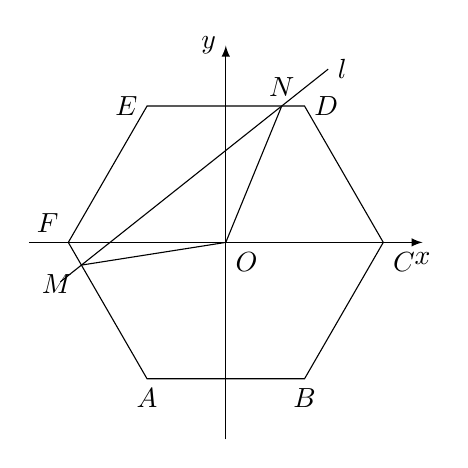
\begin{tikzpicture}[>=latex]
        \draw [->] (-2.5,0) -- (2.5,0) node [below] {$x$};
        \draw [->] (0,-2.5) -- (0,2.5) node [left] {$y$};
        \draw (0,0) node [below right] {$O$};
        \draw [name path = hexagon] (-1,{-sqrt(3)}) node [below] {$A$} -- (1,{-sqrt(3)}) node [below] {$B$} -- (2,0) node [below right] {$C$} -- (1,{sqrt(3)}) node [right] {$D$} -- (-1,{sqrt(3)}) node [left] {$E$} -- (-2,0) node [above left] {$F$} -- cycle;
        \draw [name path = linel] (-2.1,-0.5) -- (1.3,2.2)node [right] {$l$};
        \path [name intersections = {of = hexagon and linel, by = {N,M}}];
        \draw (N) node [above] {$N$} -- (0,0) -- (M) node [below left] {$M$};
    \end{tikzpicture}
\end{center}
\twoch{偶函数}{奇函数}{不是奇函数, 也不是偶函数}{奇偶性与$k$有关}


关联目标:

暂未关联目标



标签: 第二单元|第七单元

答案: A

解答或提示: 暂无解答与提示

使用记录:

20220301	2022届高三1班	\fcolorbox[rgb]{0,0,0}{1.000,0.094,0}{0.953}


出处: 2022届高三下学期测验卷01第16题
\item { (004094)}已知$f(x)$是定义在$\mathbf{R}$上的奇函数, 对任意两个不相等的正数$x_1$, $x_2$都有$\dfrac{x_2f(x_1)-x_1f(x_2)}{x_1-x_2}<0$, 则函数$g(x)=\begin{cases} \dfrac{f(x)}x, &x\ne 0, \\ 0, & x=0 \end{cases}$\bracket{20}.
\twoch{是偶函数, 且在$(0,+\infty)$上单调递减}{是偶函数, 且在$(0,+\infty)$上单调递增}{是奇函数, 且单调递减}{是奇函数, 且单调递增}


关联目标:

暂未关联目标



标签: 第二单元

答案: 暂无答案

解答或提示: 暂无解答与提示

使用记录:

20220308	2022届高三1班	\fcolorbox[rgb]{0,0,0}{1.000,0.140,0}{0.930}


出处: 2022届高三下学期测验卷02第15题
\item { (004097)}已知函数$f(x)=1-\dfrac 6{a^{x+1}+a}$($a>0$, $a\ne 1$)是定义在$\mathbf{R}$上的奇函数.\\
(1) 求实数$a$的值及函数$f(x)$的值域;\\
(2) 若不等式 $t\cdot f(x)\ge 3^x-3$在$x\in [1,2]$上恒成立, 求实数$t$的取值范围.


关联目标:

暂未关联目标



标签: 第二单元

答案: 暂无答案

解答或提示: 暂无解答与提示

使用记录:

20220308	2022届高三1班	\fcolorbox[rgb]{0,0,0}{1.000,0.032,0}{0.984}	\fcolorbox[rgb]{0,0,0}{1.000,0.104,0}{0.948}


出处: 2022届高三下学期测验卷02第18题
\item { (004108)}已知函数$f(x)=g(x)+|2x-1|$为奇函数, 若$g(-2)=7$, 则$g(2)=$\blank{50}.


关联目标:

暂未关联目标



标签: 第二单元

答案: 暂无答案

解答或提示: 暂无解答与提示

使用记录:

暂无使用记录


出处: 2022届高三下学期测验卷03第8题
\item { (004130)}已知常数$b,c\in \mathbf{R}$. 若函数$f(x)=(x^2+x-2)(x^2+bx+c)$为偶函数, 则$b+c=$\blank{50}.


关联目标:

暂未关联目标



标签: 第二单元

答案: 暂无答案

解答或提示: 暂无解答与提示

使用记录:

20220331	2022届高三1班	\fcolorbox[rgb]{0,0,0}{1.000,0.094,0}{0.953}


出处: 2022届高三下学期测验卷04第9题
\item { (004202)}已知函数$f(x)=\sqrt 2\sin (\omega x+\varphi)$, $g(x)=\sqrt 2\cos \omega x$, $\omega >0$, $\varphi \in [0,\pi)$, 它们的最小正周期为$\pi$.\\
(1) 若$y=f(x)$是奇函数, 求$f(x)$和$g(x)$在$[0,\pi]$上的公共递减区间$D$;\\
(2) 若$h(x)=f(x)+g(x)$的一个零点为$x=-\dfrac{\pi}6$, 求$h(x)$的最大值.


关联目标:

暂未关联目标



标签: 第三单元

答案: 暂无答案

解答或提示: 暂无解答与提示

使用记录:

20220428	2022届高三1班	\fcolorbox[rgb]{0,0,0}{1.000,0.086,0}{0.957}	\fcolorbox[rgb]{0,0,0}{1.000,0.172,0}{0.914}


出处: 2022届高三下学期测验卷07第18题
\item { (004203)}已知函数$f(x)=ax+\log_2(2^x+1)$, 其中$a\in \mathbf{R}$.\\
(1) 根据$a$的不同取值, 讨论$f(x)$的奇偶性, 并说明理由;\\
(2) 已知$a>0$, 函数$f(x)$的反函数为$f^{-1}(x)$, 若函数$y=f(x)+f^{-1}(x)$在区间$[1,2]$上的最小值为$1+\log_23$, 求函数$f(x)$在区间$[1,2]$上的最大值.


关联目标:

暂未关联目标



标签: 第二单元

答案: 暂无答案

解答或提示: 暂无解答与提示

使用记录:

20220428	2022届高三1班	\fcolorbox[rgb]{0,0,0}{1.000,0.032,0}{0.984}	\fcolorbox[rgb]{0,0,0}{1.000,0.466,0}{0.767}


出处: 2022届高三下学期测验卷07第19题
\item { (004224)}对于两个定义域相同的函数$f(x)$、$g(x)$, 若存在实数$m$、$n$, 使$h(x)=mf(x)+ng(x)$, 则称函数$h(x)$是由``基函数$f(x)$、$g(x)$''生成的.\\
(1) $f(x)=x^2+3x$和$g(x)=3x+4$生成一个偶函数$h(x)$, 求$h(2)$的值;\\
(2) 若$h(x)=2x^2+3x-1$由$f(x)=x^2+ax$, $g(x)=x+b$($a,b\in \mathbf{R}$且$ab\ne 0$)生成, 求$a+2b$的取值范围.


关联目标:

暂未关联目标



标签: 第二单元

答案: 暂无答案

解答或提示: 暂无解答与提示

使用记录:

20220505	2022届高三1班	\fcolorbox[rgb]{0,0,0}{1.000,0.100,0}{0.950}	\fcolorbox[rgb]{0,0,0}{1.000,0.486,0}{0.757}


出处: 2022届高三下学期测验卷08第19题
\item { (004240)}已知函数$f(x)=\cos (3x+\varphi)$满足$f(x)\le f(1)$恒成立, 则\bracket{20}.
\twoch{函数$f(x-1)$一定是奇函数}{函数$f(x+1)$一定是奇函数}{函数$f(x-1)$一定是偶函数}{函数$f(x+1)$一定是偶函数}


关联目标:

暂未关联目标



标签: 第三单元

答案: 暂无答案

解答或提示: 暂无解答与提示

使用记录:

20220512	2022届高三1班	\fcolorbox[rgb]{0,0,0}{1.000,0.094,0}{0.953}


出处: 2022届高三下学期测验卷09第14题
\item { (004256)}设$f(x)$是定义在$\mathbf{R}$上的奇函数, 当$x>0$时, $f(x)=a^x+b$($0<a<1$, $b\in \mathbf{R}$), 若$f(x)$存在反函数, 则b的取值范围是\blank{50}.


关联目标:

暂未关联目标



标签: 第二单元

答案: 暂无答案

解答或提示: 暂无解答与提示

使用记录:

20220517	2022届高三1班	\fcolorbox[rgb]{0,0,0}{1.000,0.604,0}{0.698}


出处: 2022届高三下学期测验卷10第9题
\item { (004276)}若函数$f(x)=\log_2(2^x+1)+kx$是偶函数, 则$k=$\blank{50}.


关联目标:

暂未关联目标



标签: 第二单元

答案: 暂无答案

解答或提示: 暂无解答与提示

使用记录:

20220524	2022届高三1班	\fcolorbox[rgb]{0,0,0}{1.000,0.000,0}{1.000}


出处: 2022届高三下学期测验卷11第8题
\item { (004286)}已知函数$f(x)=a-\dfrac 4{3^x+1}$($a$为实常数).\\
(1) 讨论函数$f(x)$的奇偶性, 并说明理由;\\ 
(2) 当$f(x)$为奇函数时, 对任意的$x\in [1,5]$, 不等式$f(x)\ge \dfrac u{3^x}$恒成立, 求实数$u$的最大值.


关联目标:

暂未关联目标



标签: 第二单元

答案: 暂无答案

解答或提示: 暂无解答与提示

使用记录:

20220524	2022届高三1班	\fcolorbox[rgb]{0,0,0}{1.000,0.032,0}{0.984}	\fcolorbox[rgb]{0,0,0}{1.000,0.274,0}{0.863}


出处: 2022届高三下学期测验卷11第18题
\item { (004305)}定义$F(a,b)=\begin{cases} a, & a \le b, \\ b, & a>b,\end{cases}$, 已知函数$f(x)$、$g(x)$定义域都是$\mathbf{R}$, 给出下列命题:\\
(1) 若$f(x)$、$g(x)$都是奇函数, 则函数$F(f(x),g(x))$为奇函数;\\
(2) 若$f(x)$、$g(x)$都是减函数, 则函数$F(f(x),g(x))$为减函数;\\
(3) 若$f_{\min}(x)=m$, $g_{\min}(x)=n$, 则$F_{\min}(f(x),g(x))=F(m,n)$;\\
(4) 若$f(x)$、$g(x)$都是周期函数, 则函数$F(f(x),g(x))$是周期函数.\\
其中正确命题的个数为\bracket{20}.
\fourch{$1$个}{$2$个}{$3$个}{$4$个}


关联目标:

暂未关联目标



标签: 第二单元

答案: 暂无答案

解答或提示: 暂无解答与提示

使用记录:

20220607	2022届高三1班	\fcolorbox[rgb]{0,0,0}{0.512,1.000,0}{0.256}


出处: 2022届高三下学期测验卷12第16题
\item { (004313)}设$a\in \mathbf{R}$. 若$a$使得函数$f(x)=\sqrt{8-ax-2x^2}$是偶函数, 则函数$y=f(x)$的定义域是\blank{50}.


关联目标:

暂未关联目标



标签: 第二单元

答案: 暂无答案

解答或提示: 暂无解答与提示

使用记录:

20220627	2022届高三1班	\fcolorbox[rgb]{0,0,0}{1.000,0.000,0}{1.000}


出处: 2022届高三下学期测验卷13第3题
\item { (004320)}设$a\in \mathbf{R}$. 若函数$y=f(x)$是奇函数, 且$x>0$时, $f(x)=a(x-1)+1$. 若$y=f(x)$是单调增函数, 则$a$取值范围为\blank{50}.


关联目标:

暂未关联目标



标签: 第二单元

答案: 暂无答案

解答或提示: 暂无解答与提示

使用记录:

20220627	2022届高三1班	\fcolorbox[rgb]{0,0,0}{1.000,0.140,0}{0.930}


出处: 2022届高三下学期测验卷13第10题
\item { (004329)}已知函数$f(x)=\sin x$.\\
(1) 设$a\in \mathbf{R}$, 判断函数$g(x)=a\cdot f(x)+f(x+\dfrac{\pi}2)$的奇偶性, 并说明理由;\\
(2) 设函数$F(x)=2f(x)-\sqrt 3$. 对任意$b\in \mathbf{R}$, 求$y=F(x)$在区间$[b,b+100\pi]$上零点个数的所有可能值.


关联目标:

暂未关联目标



标签: 第三单元

答案: 暂无答案

解答或提示: 暂无解答与提示

使用记录:

20220627	2022届高三1班	\fcolorbox[rgb]{0,0,0}{1.000,0.000,0}{1.000}	\fcolorbox[rgb]{0,0,0}{1.000,0.094,0}{0.953}


出处: 2022届高三下学期测验卷13第19题
\item { (004339)}已知偶函数$y=f(x)$的定义域为$\mathbf{R}$, 且当$x\ge 0$时, $f(x)=x-4$, 则不等式$xf(x)\le 5$的解为\blank{50}.


关联目标:

暂未关联目标



标签: 第二单元

答案: 暂无答案

解答或提示: 暂无解答与提示

使用记录:

20220630	2022届高三1班	\fcolorbox[rgb]{0,0,0}{1.000,0.326,0}{0.837}


出处: 2022届高三下学期测验卷14第8题
\item { (004362)}已知常数$b,c\in \mathbf{R}$. 若函数$f(x)=(x^2+x-2)(x^2+bx+c)$为偶函数, 则$b+c=$\blank{50}.


关联目标:

暂未关联目标



标签: 第二单元

答案: 暂无答案

解答或提示: 暂无解答与提示

使用记录:

20210918	2022届高三1班	\fcolorbox[rgb]{0,0,0}{1.000,0.140,0}{0.930}


出处: 2022届高三上学期测验卷01第10题
\item { (004373)}已知函数$f(x)=x|x-a|$, 其中$a$为常数.\\
(1) 当$a=1$时, 解不等式$f(x)<2$;\\
(2) 已知$g(x)$是以$2$为周期的偶函数, 且当$0\le x\le 1$时, 有$g(x)=f(x)$. 若$a<0$, 且$g(\dfrac 32)=\dfrac 54$, 求函数$y=g(x)$($x\in [1,2]$)的反函数;\\
(3) 若在$[0,2]$上存在$n$个不同的点$x_i$($i=1,2,\cdots,n$, $n\ge 3$), $x_1<x_2<\cdots <x_n$, 使得$|f(x_1)-f(x_2)|+|f(x_2)-f(x_3)|+\cdots+|f(x_{n-1})-f(x_n)|=8$, 求实数$a$的取值范围.


关联目标:

暂未关联目标



标签: 第二单元

答案: 暂无答案

解答或提示: 暂无解答与提示

使用记录:

20210918	2022届高三1班	\fcolorbox[rgb]{0,0,0}{1.000,0.070,0}{0.965}	\fcolorbox[rgb]{0,0,0}{1.000,0.574,0}{0.713}	\fcolorbox[rgb]{0,0,0}{0.220,1.000,0}{0.110}


出处: 2022届高三上学期测验卷01第21题
\item { (004375)}已知常数$a\in \mathbf{R}$, 函数$f(x)=x^2$($-1\le x\le a$)是偶函数, 则$a=$\blank{50}.


关联目标:

暂未关联目标



标签: 第二单元

答案: 暂无答案

解答或提示: 暂无解答与提示

使用记录:

20210928	2022届高三1班	\fcolorbox[rgb]{0,0,0}{1.000,0.000,0}{1.000}


出处: 2022届高三上学期测验卷02第2题
\item { (004386)}已知常数$a\in \mathbf{R}$, 函数$f(x)=ax^2+\lg \dfrac{1+x}{1-x}$.\\
(1) 若$a=0$, 判断$f(x)$的单调性并证明;\\
(2) 问: 是否存在$a$, 使得$f(x)$为奇函数? 若存在, 求出所有$a$的值; 若不存在, 说明理由.


关联目标:

暂未关联目标



标签: 第二单元

答案: 暂无答案

解答或提示: 暂无解答与提示

使用记录:

20210928	2022届高三1班	\fcolorbox[rgb]{0,0,0}{1.000,0.290,0}{0.855}	\fcolorbox[rgb]{0,0,0}{1.000,0.082,0}{0.959}


出处: 2022届高三上学期测验卷02第13题
\item { (004395)}$f(x)$是偶函数, 当$x\ge 0$时, $f(x)=2^x-1$, 则不等式$f(x)>1$的解集为\blank{50}.


关联目标:

暂未关联目标



标签: 第二单元

答案: 暂无答案

解答或提示: 暂无解答与提示

使用记录:

20211012	2022届高三1班	\fcolorbox[rgb]{0,0,0}{1.000,0.000,0}{1.000}


出处: 2022届高三上学期测验卷03第8题
\item { (004407)}已知函数$f(x)=\dfrac{ax^2+1}{bx+c}$是奇函数, $a,b,c$为常数.\\
(1)	求实数$c$的值;\\
(2)	若$a,b\in \mathbf{Z}$, 且$f(1)=2$, $f(2)<3$, 求$f(x)$的解析式;\\
(3) 已知$b>0$, 若$f(x)\ge f(1)$在$(0,+\infty)$上恒成立, 且$\{x|f[f(x)]\ge x\}\cap [1,2]\ne \varnothing$, 求$b$的取值范围.


关联目标:

暂未关联目标



标签: 第二单元

答案: 暂无答案

解答或提示: 暂无解答与提示

使用记录:

20211012	2022届高三1班	\fcolorbox[rgb]{0,0,0}{1.000,0.212,0}{0.894}	\fcolorbox[rgb]{0,0,0}{1.000,0.110,0}{0.945}	\fcolorbox[rgb]{0,0,0}{1.000,0.880,0}{0.560}


出处: 2022届高三上学期测验卷03第20题
\item { (004436)}若定义在实数集$\mathbf{R}$上的奇函数$y=f(x)$的图像关于直线$x=1$对称, 且当$0\le x\le 1$时, $f(x)=x^{\frac 13}$, 则方程$f(x)=\dfrac 13$在区间$(-4,10)$内的所有实根之和为\blank{50}.


关联目标:

暂未关联目标



标签: 第二单元

答案: 暂无答案

解答或提示: 暂无解答与提示

使用记录:

20211026	2022届高三1班	\fcolorbox[rgb]{0,0,0}{1.000,0.326,0}{0.837}


出处: 2022届高三上学期测验卷05第12题
\item { (004456)}在高中阶段, 我们学习过函数的概念、性质和图像, 以下两个结论是正确的: \textcircled{1} 偶函数$f(x)$在区间$[a,b]$($a<b$)上的取值范围与在区间$[-b,-a]$上的取值范围是相等的. \textcircled{2} 周期函数$f(x)$在一个周期内的取值范围也就是$f(x)$在定义域上的值域. 由此可求函数$g(x)=2|\sin x|+19|\cos x|$的值域为\blank{50}.


关联目标:

暂未关联目标



标签: 第三单元

答案: 暂无答案

解答或提示: 暂无解答与提示

使用记录:

20211102	2022届高三1班	\fcolorbox[rgb]{0,0,0}{1.000,0.572,0}{0.714}


出处: 2022届高三上学期测验卷06第11题
\item { (004457)}定义在实数集$\mathbf{R}$上的偶函数$f(x)$满足$f(x+1)=1+\sqrt{2f(x)-f^2(x)}$, 则$f(\dfrac{2019}{2})=$\blank{50}.


关联目标:

暂未关联目标



标签: 第二单元

答案: 暂无答案

解答或提示: 暂无解答与提示

使用记录:

20211102	2022届高三1班	\fcolorbox[rgb]{0,0,0}{1.000,0.572,0}{0.714}


出处: 2022届高三上学期测验卷06第12题
\item { (004464)}已知$a$是实常数, 函数$f(x)=a\lg(1-x)-\lg (1+x)$.\\
(1) 若$a=1$, 求证: 函数$y=f(x)$是减函数;\\
(2) 讨论函数$f(x)$的奇偶性, 并说明理由.


关联目标:

暂未关联目标



标签: 第二单元

答案: 暂无答案

解答或提示: 暂无解答与提示

使用记录:

20211102	2022届高三1班	\fcolorbox[rgb]{0,0,0}{1.000,0.126,0}{0.937}	\fcolorbox[rgb]{0,0,0}{1.000,0.108,0}{0.946}


出处: 2022届高三上学期测验卷06第19题
\item { (004474)}已知$\omega,t>0$, 函数$f(x)=\begin{vmatrix}
\sqrt 3 & \sin \omega x  \\ 1  & \cos \omega x  \end{vmatrix}$的最小正周期为$2\pi$, 将$f(x)$的图像向左平移$t$个单位, 所得图像对应的函数为偶函数, 则$t$的最小值为\blank{50}.


关联目标:

暂未关联目标



标签: 暂无对应

答案: 暂无答案

解答或提示: 暂无解答与提示

使用记录:

20211116	2022届高三1班	\fcolorbox[rgb]{0,0,0}{1.000,0.326,0}{0.837}


出处: 2022届高三上学期测验卷07第8题
\item { (004525)}已知函数$f(x)=\begin{cases} x^2, & x\text{为无理数}, \\ x, &x\text{为有理数},   \end{cases}$ 则以下$4$个命题:
\textcircled{1} $f(x)$是偶函数; \textcircled{2} $f(x)$在$[0,+\infty)$上是增函数; \textcircled{3} $f(x)$的值域为$\mathbf{R}$; \textcircled{4} 对于任意的正有理数$a$, $g(x)=f(x)-a$存在奇数个零点.
其中正确命题的个数为\bracket{20}.
\fourch{$0$}{$1$}{$2$}{$3$}


关联目标:

暂未关联目标



标签: 第二单元

答案: 暂无答案

解答或提示: 暂无解答与提示

使用记录:

20211129	2022届高三1班	\fcolorbox[rgb]{0,0,0}{1.000,0.326,0}{0.837}


出处: 2022届高三上学期测验卷09第16题
\item { (004540)}已知$y=f(x)$是定义在$\mathbf{R}$上的奇函数, 且当$x\ge 0$时, $f(x)=-\dfrac 1{4^x}+\dfrac 1{2^x}$, 则此函数的值域为\blank{50}.


关联目标:

暂未关联目标



标签: 第二单元

答案: 暂无答案

解答或提示: 暂无解答与提示

使用记录:

20211214	2022届高三1班	\fcolorbox[rgb]{0,0,0}{1.000,0.232,0}{0.884}


出处: 2022届高三上学期测验卷10第10题
\item { (004544)}设函数$f(x)=\begin{cases}1, & x\in \mathbf{Q}, \\ \pi, &x\not\in \mathbf{Q}.\end{cases}$ 下列结论不正确的是\bracket{20}.
\twoch{$f(x)$是偶函数}{$f(x)$是周期函数}{该函数有最大值也有最小值}{方程$f(f(x))=1$的解集为$\{1\}$}


关联目标:

暂未关联目标



标签: 第二单元

答案: 暂无答案

解答或提示: 暂无解答与提示

使用记录:

20211214	2022届高三1班	\fcolorbox[rgb]{0,0,0}{1.000,0.140,0}{0.930}


出处: 2022届高三上学期测验卷10第14题
\item { (004622)}若$f(x)$是奇函数, 且当$x\ge 0$时, $f(x)=x^2+x$, 则当$x<0$时, $f(x)=$\blank{50}.


关联目标:

暂未关联目标



标签: 第二单元

答案: 暂无答案

解答或提示: 暂无解答与提示

使用记录:

20210924	2022届高三1班	\fcolorbox[rgb]{0,0,0}{1.000,0.182,0}{0.909}

20210924	2022届高三	\fcolorbox[rgb]{0,0,0}{1.000,0.206,0}{0.897}


出处: 2022届高三上月考卷01第4题
\item { (004671)}设$f(x)$是定义在$\mathbf{R}$上的函数, 且满足$f(1)=0$.若$y=f(x)+a\cdot 2^x$是奇函数, $y=f(x)+3^x$是偶函数, 则$a$的值为\blank{50}.


关联目标:

暂未关联目标



标签: 第二单元

答案: 暂无答案

解答或提示: 暂无解答与提示

使用记录:

20211109	2022届高三	\fcolorbox[rgb]{0,0,0}{1.000,0.402,0}{0.799}


出处: 2022届高三上期中区统考第11题
\item { (004674)}下列函数中, 既是奇函数, 又是减函数的是\bracket{20}.
\fourch{$y=x^{-1}$}{$y=-\arcsin x$}{$y=\log_2x$}{$y=2^x$}


关联目标:

暂未关联目标



标签: 第三单元

答案: 暂无答案

解答或提示: 暂无解答与提示

使用记录:

20211109	2022届高三	\fcolorbox[rgb]{0,0,0}{1.000,0.130,0}{0.935}


出处: 2022届高三上期中区统考第14题
\item { (004680)}已知函数$f(x)=2^x+\dfrac a{2^x}$, $a$为实常数.\\
(1) 若函数$f(x)$为奇函数, 求$a$的值;\\
(2) 若$x\in [0,1]$时$f(x)$的最小值为$2$, 求$a$的值;\\
(3) 若方程$f(x)=6$有两个不等的实根$x_1,x_2$, 且$|x_1-x_2|\le 1$, 求$a$的取值范围.


关联目标:

暂未关联目标



标签: 第二单元

答案: 暂无答案

解答或提示: 暂无解答与提示

使用记录:

20211109	2022届高三	\fcolorbox[rgb]{0,0,0}{1.000,0.234,0}{0.883}	\fcolorbox[rgb]{0,0,0}{1.000,0.340,0}{0.830}	\fcolorbox[rgb]{0,0,0}{1.000,0.906,0}{0.547}


出处: 2022届高三上期中区统考第20题
\item { (004697)}已知非空集合$A,B$满足: $A\cup B=R$, $A\cap B=\varnothing$, 函数$f(x)=\begin{cases}
x^2, &  x\in A,  \\ 2x-1, &  x\in B.  \end{cases}$ 对于下列两个命题: \textcircled{1} 存在唯一的非空集合对$(A,B)$, 使得$f(x)$为偶函数; \textcircled{2} 存在无穷多非空集合对$(A,B)$, 使得方程$f(x)=2$无解. 下面判断正确的是\bracket{20}.
\fourch{\textcircled{1} 正确, \textcircled{2} 错误}{\textcircled{1} 错误, \textcircled{2} 正确}{\textcircled{1} 、\textcircled{2} 都正确}{\textcircled{1} 、\textcircled{2} 都错误}


关联目标:

K0217004B|D02003B|会运用奇函数、偶函数的定义, 证明一些较为简单的函数是奇函数或是偶函数.

K0223002B|D02004B|会用函数的观点求解一元二次方程.



标签: 第一单元|第二单元

答案: 暂无答案

解答或提示: 暂无解答与提示

使用记录:

20211221	2022届高三	\fcolorbox[rgb]{0,0,0}{1.000,0.932,0}{0.534}


出处: 2022届高三上一模第16题
\item { (004731)}已知集合$A=\{-2,-1,-\dfrac 12,\dfrac 13,\dfrac 12,1,2,3\}$, 从集合$A$中任取一个元素$a$, 使函数$y=x^a$是奇函数且在$(0,+\infty)$上递增的概率为\blank{50}.


关联目标:

暂未关联目标



标签: 第二单元|第八单元

答案: 暂无答案

解答或提示: 暂无解答与提示

使用记录:

20220621	2022届高三	\fcolorbox[rgb]{0,0,0}{1.000,0.230,0}{0.885}


出处: 2022届高三下二模第8题
\item { (004741)}已知函数$f(x)=t\sin x+|\cos x|$, 其中常数$t\in \mathbf{R}$.\\
(1) 讨论函数$f(x)$的奇偶性, 并说明理由;\\
(2) $\triangle ABC$中内角$A,B,C$所对的边分别为$a,b,c$, 且$a=2$, $b=\sqrt 5$, $f(A)=2$, 求当$t=\sqrt 3$时, $\triangle ABC$的面积.


关联目标:

暂未关联目标



标签: 第三单元

答案: 暂无答案

解答或提示: 暂无解答与提示

使用记录:

20220621	2022届高三	\fcolorbox[rgb]{0,0,0}{1.000,0.208,0}{0.896}	\fcolorbox[rgb]{0,0,0}{1.000,0.202,0}{0.899}


出处: 2022届高三下二模第18题
\item { (004757)}下列函数中既是奇函数, 又在区间$(0,+\infty)$上单调递减的函数为\bracket{20}.
\fourch{$y=\sqrt x$}{$y=\log_{\frac 12}x$}{$y=-x^3$}{$y=x+\dfrac 1x$}


关联目标:

暂未关联目标



标签: 第二单元

答案: 暂无答案

解答或提示: 暂无解答与提示

使用记录:

20220317	2022届高三1班	\fcolorbox[rgb]{0,0,0}{1.000,0.000,0}{1.000}


出处: 2022届高三下月考卷01第13题
\item { (005360)}已知奇函数$y=f(x)$在$x<0$时是减函数, 求证: $y=f(x)$在$x>0$时也是减函数.


关联目标:

暂未关联目标



标签: 第二单元

答案: 暂无答案

解答或提示: 暂无解答与提示

使用记录:

暂无使用记录


出处: 代数精编第三章函数
\item { (005361)}已知$f(x)$是奇函数, 且当$x>0$时$f(x)=x(1-x)$, 求$f(x)$在$x<0$时的表达式.


关联目标:

暂未关联目标



标签: 第二单元

答案: 暂无答案

解答或提示: 暂无解答与提示

使用记录:

暂无使用记录


出处: 代数精编第三章函数
\item { (005491)}若$f(x)=(m-1)x^2+3mx+3$为偶函数, 则$f(x)$在区间$(-4,2)$上\bracket{20}.
\twoch{是增函数}{是减函数}{先是增函数后是减函数}{先是减函数后是增函数}


关联目标:

暂未关联目标



标签: 第二单元

答案: 暂无答案

解答或提示: 暂无解答与提示

使用记录:

暂无使用记录


出处: 代数精编第三章函数
\item { (005492)}函数$f(x)=\begin{cases}   1-x, & x>0,  \\ 0, & x=0,  \\1+x, & x<0,  \end{cases}$则该函数\bracket{20}.
\twoch{是奇函数, 但不是偶函数}{是偶函数, 但不是奇函数}{既是奇函数, 也是偶函数}{既不是奇函数, 也不是偶函数}


关联目标:

暂未关联目标



标签: 第二单元

答案: 暂无答案

解答或提示: 暂无解答与提示

使用记录:

暂无使用记录


出处: 代数精编第三章函数
\item { (005493)}下列函数中既是奇函数, 又在定义域上为增函数的是\bracket{20}.
\fourch{$f(x)=3x+1$}{$f(x)=\dfrac 1x$}{$f(x)=1-\dfrac 1x$}{$f(x)=x^3$}


关联目标:

暂未关联目标



标签: 第二单元

答案: 暂无答案

解答或提示: 暂无解答与提示

使用记录:

暂无使用记录


出处: 代数精编第三章函数
\item { (005494)}若$f(x)$为定义在区间$[-6, 6]$上的偶函数, 且满足$f(3)>f(1)$, 则恒成立的是\bracket{20}.
\fourch{$f(-1)<f(3)$}{$f(0)<f(6)$}{$f(3)>f(2)$}{$f(2)>f(0)$}


关联目标:

暂未关联目标



标签: 第二单元

答案: 暂无答案

解答或提示: 暂无解答与提示

使用记录:

暂无使用记录


出处: 代数精编第三章函数
\item { (005495)}函数$f(x)=\dfrac{\sqrt {1-x^2}}{2-|x+2|}$\bracket{20}.
\twoch{是奇函数, 但不是偶函数}{是偶函数, 但不是奇函数}{既是奇函数, 又是偶函数}{既不是奇函数, 也不是偶函数}


关联目标:

暂未关联目标



标签: 第二单元

答案: 暂无答案

解答或提示: 暂无解答与提示

使用记录:

暂无使用记录


出处: 代数精编第三章函数
\item { (005496)}已知$f(x)$是奇函数, 则下列各点中在函数$y=f(x)$的图像上的点的是\bracket{20}.
\fourch{$(a,f(-a))$}{$(-a,-f(a))$}{$(\dfrac 1a,-f(\dfrac 1a))$}{$(-\sin a,-f(-\sin a))$}


关联目标:

暂未关联目标



标签: 第二单元

答案: 暂无答案

解答或提示: 暂无解答与提示

使用记录:

暂无使用记录


出处: 代数精编第三章函数
\item { (005497)}若$f(x)$是定义在$\mathbf{R}$上的偶函数, 且当$x<0$时, $f(x)=2x-3$, 则当$x>0$时, $f(x)=$\blank{50}.


关联目标:

暂未关联目标



标签: 第二单元

答案: 暂无答案

解答或提示: 暂无解答与提示

使用记录:

暂无使用记录


出处: 代数精编第三章函数
\item { (005498)}若奇函数$f(x)$的定义域是$\mathbf{R}$, 则$f(0)=$\blank{50}.


关联目标:

暂未关联目标



标签: 第二单元

答案: 暂无答案

解答或提示: 暂无解答与提示

使用记录:

暂无使用记录


出处: 代数精编第三章函数
\item { (005499)}若奇函数$f(x)$在区间$[-3, -1]$上是增函数, 且有最大值$-2$, 则$f(x)$在$[1, 3]$上是\blank{50}函数(填``增''或``减''), 且最小值等于\blank{50}.


关联目标:

暂未关联目标



标签: 第二单元

答案: 暂无答案

解答或提示: 暂无解答与提示

使用记录:

暂无使用记录


出处: 代数精编第三章函数
\item { (005500)}设$f(x)$为定义在$\mathbf{R}$上的偶函数, 且$f(x)$在$[0,+\infty)$上是增函数, 则$f(-4)$, $f(-2)$, $f(3)$由小到大的排列顺序为\blank{50}.


关联目标:

暂未关联目标



标签: 第二单元

答案: 暂无答案

解答或提示: 暂无解答与提示

使用记录:

暂无使用记录


出处: 代数精编第三章函数
\item { (005502)}设$f(x)$在$R$上是奇函数, 且当$x\in [0,+\infty)$时, $f(x)=x(1+\sqrt[3]x)$, 那么当$x\in (-\infty ,0)$时, $f(x)=$\bracket{20}.
\fourch{$-x(1+\sqrt[3]x)$}{$x(1+\sqrt[3]x)$}{$-x(1-\sqrt[3]x)$}{$x(1-\sqrt[3]x)$}


关联目标:

暂未关联目标



标签: 第二单元

答案: 暂无答案

解答或提示: 暂无解答与提示

使用记录:

暂无使用记录


出处: 代数精编第三章函数
\item { (005504)}函数$f(x)=x|x|-2x$是\bracket{20}.
\twoch{偶函数, 且在(-1, 1)上是增函数}{奇函数, 且在(-1, 1)上是减函数}{偶函数, 且在(-1, 1)上是减函数}{奇函数, 且在(-1, 1)上是增函数}


关联目标:

暂未关联目标



标签: 第二单元

答案: 暂无答案

解答或提示: 暂无解答与提示

使用记录:

暂无使用记录


出处: 代数精编第三章函数
\item { (005505)}若函数$y=f(x)$是偶函数, 其图像与$x$轴有四个交点, 则方程$f(x)=0$的所有实数根之和为\bracket{20}.
\fourch{$4$}{$2$}{$1$}{$0$}


关联目标:

暂未关联目标



标签: 第二单元

答案: 暂无答案

解答或提示: 暂无解答与提示

使用记录:

暂无使用记录


出处: 代数精编第三章函数
\item { (005506)}函数$f(x)=\dfrac x{2^{1+x}+2^{1-x}}$\bracket{20}.
\twoch{是奇函数, 但不是偶函数}{是偶函数, 但不是奇函数}{既是奇函数, 又是偶函数}{既不是奇函数, 也不是偶函数}


关联目标:

暂未关联目标



标签: 第二单元

答案: 暂无答案

解答或提示: 暂无解答与提示

使用记录:

暂无使用记录


出处: 代数精编第三章函数
\item { (005507)}已知奇函数$f(x)$在$x>0$时的表达式为$f(x)=2x-\dfrac 12$, 则当$x\le -\dfrac 14$时, 恒有\bracket{20}.
\fourch{$f(x)>0$}{$f(x)<0$}{$f(x)-f(-x)\le 0$}{$f(x)-f(-x)>0$}


关联目标:

暂未关联目标



标签: 第二单元

答案: 暂无答案

解答或提示: 暂无解答与提示

使用记录:

暂无使用记录


出处: 代数精编第三章函数
\item { (005509)}已知$f(x),g(x)$都是定义在$\mathbf{R}$上的函数, $f(x)$为奇函数, $g(x)$为偶函数, 且$f(x)\cdot g(x)$恒不为$0$, 判断下列函数的奇偶性:
(1)$f(x)+g(x)$:\blank{50}; (2)$f(x)\cdot g(x)$:\blank{50}; (3)$f[f(x)]$:\blank{50}; (4)$f[g(x)]$:\blank{50}; (5)$g[f(x)]$:\blank{50}; (6)$g[g(x)]$:\blank{50}.


关联目标:

暂未关联目标



标签: 第二单元

答案: 暂无答案

解答或提示: 暂无解答与提示

使用记录:

暂无使用记录


出处: 代数精编第三章函数
\item { (005510)}判断函数$f(x)=5$的奇偶性:\blank{50}.


关联目标:

暂未关联目标



标签: 第二单元

答案: 暂无答案

解答或提示: 暂无解答与提示

使用记录:

暂无使用记录


出处: 代数精编第三章函数
\item { (005511)}判断函数$f(x)=\sqrt {x^2-1}+\sqrt {1-x^2}$的奇偶性:\blank{50}.


关联目标:

暂未关联目标



标签: 第二单元

答案: 暂无答案

解答或提示: 暂无解答与提示

使用记录:

暂无使用记录


出处: 代数精编第三章函数
\item { (005512)}判断函数$f(x)=x^2-2x^2+3$的奇偶性:\blank{50}.


关联目标:

暂未关联目标



标签: 第二单元

答案: 暂无答案

解答或提示: 暂无解答与提示

使用记录:

暂无使用记录


出处: 代数精编第三章函数
\item { (005513)}判断函数$x\in [-4,4)$的奇偶性:\blank{50}.


关联目标:

暂未关联目标



标签: 第二单元

答案: 暂无答案

解答或提示: 暂无解答与提示

使用记录:

暂无使用记录


出处: 代数精编第三章函数
\item { (005514)}判断函数$f(x)=|3x+2|-|3x-2|$的奇偶性:\blank{50}.


关联目标:

暂未关联目标



标签: 第二单元

答案: 暂无答案

解答或提示: 暂无解答与提示

使用记录:

暂无使用记录


出处: 代数精编第三章函数
\item { (005515)}判断函数$f(x)=\dfrac{x^2(x-1)}{x-1}$的奇偶性:\blank{50}.


关联目标:

暂未关联目标



标签: 第二单元

答案: 暂无答案

解答或提示: 暂无解答与提示

使用记录:

暂无使用记录


出处: 代数精编第三章函数
\item { (005516)}判断函数$f(x)=\dfrac 12[g(x)-g(-x)]$的奇偶性:\blank{50}.


关联目标:

暂未关联目标



标签: 第二单元

答案: 暂无答案

解答或提示: 暂无解答与提示

使用记录:

暂无使用记录


出处: 代数精编第三章函数
\item { (005517)}求证: 函数$f(x)=\dfrac{x+1+\sqrt {1+x^2}}{x-1+\sqrt {1+x^2}}$是奇函数.


关联目标:

暂未关联目标



标签: 第二单元

答案: 暂无答案

解答或提示: 暂无解答与提示

使用记录:

暂无使用记录


出处: 代数精编第三章函数
\item { (005518)}求证: 函数$f(x)=\begin{cases}
   x(1-x), &  x>0,  \\ x(1+x), &  x<0  \end{cases}$是奇函数.


关联目标:

暂未关联目标



标签: 第二单元

答案: 暂无答案

解答或提示: 暂无解答与提示

使用记录:

暂无使用记录


出处: 代数精编第三章函数
\item { (005519)}已知奇函数$f(x)$在定义域$(-l, l)$上是减函数, 求满足$f(1-m)+f(1-m^2)<0$的实数$m$的取值范围.


关联目标:

暂未关联目标



标签: 第二单元

答案: 暂无答案

解答或提示: 暂无解答与提示

使用记录:

暂无使用记录


出处: 代数精编第三章函数
\item { (005520)}已知偶函数$f(x)$在$[0,+\infty)$上是增函数.求不等式$f(2x+5)<f(x^2+2)$的解集.


关联目标:

暂未关联目标



标签: 第二单元

答案: 暂无答案

解答或提示: 暂无解答与提示

使用记录:

暂无使用记录


出处: 代数精编第三章函数
\item { (005521)}是否存在既是奇函数又是偶函数的函数? 说明理由


关联目标:

暂未关联目标



标签: 第二单元

答案: 暂无答案

解答或提示: 暂无解答与提示

使用记录:

暂无使用记录


出处: 代数精编第三章函数
\item { (005522)}求证: 定义域为$(-l,l)$的任何函数都能表示成一个奇函数与一个偶函数之和.


关联目标:

暂未关联目标



标签: 第二单元

答案: 暂无答案

解答或提示: 暂无解答与提示

使用记录:

暂无使用记录


出处: 代数精编第三章函数
\item { (005544)}若幂函数$f(x)$是奇函数, 则$f^{-1}(1)=$\blank{50}, $f^{-1}(-1)=$\blank{50}.


关联目标:

暂未关联目标



标签: 第二单元

答案: 暂无答案

解答或提示: 暂无解答与提示

使用记录:

暂无使用记录


出处: 代数精编第三章函数
\item { (005594)}若$f(x)=a+\dfrac 1{4^x+1}$是奇函数, 求常数$a$的值.


关联目标:

暂未关联目标



标签: 第二单元

答案: 暂无答案

解答或提示: 暂无解答与提示

使用记录:

暂无使用记录


出处: 代数精编第三章函数
\item { (005595)}若$f(x)=x^2(\dfrac 1{a^x-1}+m)$($a>0$且$a\ne 1$)为奇函数, 求常数$m$的值.


关联目标:

暂未关联目标



标签: 第二单元

答案: 暂无答案

解答或提示: 暂无解答与提示

使用记录:

暂无使用记录


出处: 代数精编第三章函数
\item { (005596)}已知函数$f(x)=(\dfrac 1{2^x-1}+\dfrac 12)x^3$.\\
(1) 求函数的定义域;\\
(2) 讨论$f(x)$的奇偶性;\\
(3) 求证: $f(x)>0$.


关联目标:

暂未关联目标



标签: 第二单元

答案: 暂无答案

解答或提示: 暂无解答与提示

使用记录:

暂无使用记录


出处: 代数精编第三章函数
\item { (005597)}已知$f(x)=\dfrac{a^x-1}{a^x+1}$($a>1$).\\
(1) 判断函数$f(x)$的奇偶性;\\
(2) 求函数$f(x)$的值域;\\
(3) 求证: $f(x)$在区间$(-\infty ,+\infty)$上是增函数.


关联目标:

暂未关联目标



标签: 第二单元

答案: 暂无答案

解答或提示: 暂无解答与提示

使用记录:

暂无使用记录


出处: 代数精编第三章函数
\item { (005691)}设$f(x)$是定义在$(-\infty ,+\infty)$上的偶函数, 且它在$[0,+\infty)$上是增函数, 记$a=f(-\log_{\sqrt 2}\sqrt 3)$, $b=f(-\log_{\sqrt 3}\sqrt 2)$, $c=f(-2)$, 则$a,b,c$的大小关系是\bracket{20}.
\fourch{$a>b>c$}{$b>c>a$}{$c>a>b$}{$c>b>a$}


关联目标:

暂未关联目标



标签: 第二单元

答案: 暂无答案

解答或提示: 暂无解答与提示

使用记录:

暂无使用记录


出处: 代数精编第三章函数
\item { (005713)}函数$y=\lg \dfrac{1-x}{1+x}$\bracket{20}.
\twoch{是奇函数, 且在$(-1, 1)$是增函数}{是奇函数, 且在$(-1, 1)$上是减函数}{是偶函数, 且在$(-1, 1)$是增函数}{是偶函数, 且在$(-1, 1)$上是减函数}


关联目标:

暂未关联目标



标签: 第二单元

答案: 暂无答案

解答或提示: 暂无解答与提示

使用记录:

暂无使用记录


出处: 代数精编第三章函数
\item { (005714)}函数$f(x)=\ln (\mathrm{e}^x+1)-\dfrac x2$\bracket{20}.
\twoch{是奇函数, 但不是偶函数}{是偶函数, 但不是奇函数}{既是奇函数, 又是偶函数}{没有奇偶性}


关联目标:

暂未关联目标



标签: 第二单元

答案: 暂无答案

解答或提示: 暂无解答与提示

使用记录:

暂无使用记录


出处: 代数精编第三章函数
\item { (005742)}实数$a$为何值时, 函数$f(x)=2^x-2^{-x}\lg a$为奇函数?


关联目标:

暂未关联目标



标签: 第二单元

答案: 暂无答案

解答或提示: 暂无解答与提示

使用记录:

暂无使用记录


出处: 代数精编第三章函数
\item { (005750)}已知函数$f(x)=\log_a\dfrac{x+b}{x-b}$($a>0$, $b>0$且$a\ne 1$).\\
(1) 求$f(x)$的定义域;\\
(2) 讨论$f(x)$的奇偶性;\\
(3) 讨论$f(x)$的单调性;\\
(4) 求$f(x)$的反函数$f^{-1}(x)$.


关联目标:

暂未关联目标



标签: 第二单元

答案: 暂无答案

解答或提示: 暂无解答与提示

使用记录:

暂无使用记录


出处: 代数精编第三章函数
\item { (005830)}已知$f(x+y)=f(x)+f(y)$对于任何实数$x,y$都成立.\\
(1) 求证: $f(2x)=2f(x)$;\\
(2) 求$f(0)$的值;\\
(3) 求证: $f(x)$为奇函数.


关联目标:

暂未关联目标



标签: 第二单元

答案: 暂无答案

解答或提示: 暂无解答与提示

使用记录:

暂无使用记录


出处: 代数精编第三章函数
\item { (005831)}已知函数$f(x)$对任何实数$x,y$满足$f(x+y)+f(x-y)=2f(x)f(y)$, 且$f(0)\ne 0$, 求证: $f(x)$是偶函数.


关联目标:

暂未关联目标



标签: 第二单元

答案: 暂无答案

解答或提示: 暂无解答与提示

使用记录:

暂无使用记录


出处: 代数精编第三章函数
\item { (005832)}已知函数$f(x)$($x\ne 0$)满足$f(xy)=f(x)+f(y)$.
(1) 求证: $f(1)=f(-1)=0$;\\
(2) 求证: $f(x)$为偶函数;\\
(3) 若$f(x)$在$(0,+\infty)$上是增函数, 解不等式$f(x)+f(x-\dfrac 12)\le 0$.


关联目标:

暂未关联目标



标签: 第二单元

答案: 暂无答案

解答或提示: 暂无解答与提示

使用记录:

暂无使用记录


出处: 代数精编第三章函数
\item { (005847)}已知函数$f(2x+1)$是偶函数, 求函数$f(2x)$的图像的对称轴.


关联目标:

暂未关联目标



标签: 第二单元

答案: 暂无答案

解答或提示: 暂无解答与提示

使用记录:

暂无使用记录


出处: 代数精编第三章函数
\item { (005855)}已知$f(x)$在$(-\infty ,+\infty)$上有单调性, 且满足$f(1)=2$和$f(x+y)=f(x)+f(y)$.\\
(1) 求证: $f(x)$为奇函数;\\
(2) 若$f(x)$满足$f(k\log_2t)+f(\log_2t-\log_2^2t-2)<0$, 求实数$k$的取值范围.


关联目标:

暂未关联目标



标签: 第二单元

答案: 暂无答案

解答或提示: 暂无解答与提示

使用记录:

暂无使用记录


出处: 代数精编第三章函数
\item { (005968)}函数$y=\cos (\tan x)$\bracket{20}.
\twoch{是奇函数, 但不是偶函数}{是偶函数, 但不是奇函数}{既不是奇函数, 也不是偶函数}{奇偶性无法确定}


关联目标:

暂未关联目标



标签: 第三单元

答案: 暂无答案

解答或提示: 暂无解答与提示

使用记录:

暂无使用记录


出处: 代数精编第四章三角函数
\item { (006000)}函数$y=\lg (1-\sin x)-\lg (1+\sin x)$(.)
\twoch{是奇函数, 但非偶函数}{是偶函数, 但非奇函数}{既不是奇函数, 也不是偶函数}{奇偶性无法确定}


关联目标:

暂未关联目标



标签: 第三单元

答案: 暂无答案

解答或提示: 暂无解答与提示

使用记录:

暂无使用记录


出处: 代数精编第四章三角函数
\item { (006002)}若函数$y=\cos (\sin x)$, 则下列结论正确的是\bracket{20}.
\fourch{它的定义域是[-1, 1]}{它是奇函数}{它的值域是$[\cos 1,1]$}{它不是周期函数}


关联目标:

暂未关联目标



标签: 第三单元

答案: 暂无答案

解答或提示: 暂无解答与提示

使用记录:

暂无使用记录


出处: 代数精编第四章三角函数
\item { (006003)}下列四个函数中, 是偶函数且在$[0,\dfrac{\pi}2]$上为增函数, 但不是周期函数的函数是\bracket{20}.
\twoch{$y=|\sin x|$($x\in \mathbf{R}$)}{$y=|\cos x|$($x\in \mathbf{R}$)}{$y=\sin|x|$($x\in \mathbf{R}$)}{$y=|\sin x|+|\cos x|$($x\in \mathbf{R}$)}


关联目标:

暂未关联目标



标签: 第三单元

答案: 暂无答案

解答或提示: 暂无解答与提示

使用记录:

暂无使用记录


出处: 代数精编第四章三角函数
\item { (006004)}下列函数中, 既在$(0,\dfrac{\pi}2)$上是增函数, 又是以$\pi$为最小正周期的偶函数是\bracket{20}.
\fourch{$y=x^2|\cos x|$}{$y=\cos 2x$}{$y=|\sin x|$}{$y=|\sin 2x|$}


关联目标:

暂未关联目标



标签: 第三单元

答案: 暂无答案

解答或提示: 暂无解答与提示

使用记录:

暂无使用记录


出处: 代数精编第四章三角函数
\item { (006048)}将奇函数$y=f(x)$($x\in \mathbf{R}$)的图像沿$x$轴正向平移$1$个单位长度后, 所得的图像为$C'$, 而图像$C'$与$C$关于原点对称, 那么$C$所对应的函数应为\blank{50}.


关联目标:

暂未关联目标



标签: 第三单元

答案: 暂无答案

解答或提示: 暂无解答与提示

使用记录:

暂无使用记录


出处: 代数精编第四章三角函数
\item { (006051)}若函数$f(x)=\sin (2x+\varphi)$($-\pi <\varphi <0$)是偶函数, 则$\varphi =$\blank{50}.


关联目标:

暂未关联目标



标签: 第三单元

答案: 暂无答案

解答或提示: 暂无解答与提示

使用记录:

暂无使用记录


出处: 代数精编第四章三角函数
\item { (006054)}若奇函数$f(x)$是最小正周期为$3$的周期函数, 且$f(1)=-1$, 则$f(101)=$\blank{50}.


关联目标:

暂未关联目标



标签: 第三单元

答案: 暂无答案

解答或提示: 暂无解答与提示

使用记录:

暂无使用记录


出处: 代数精编第四章三角函数
\item { (006055)}若偶函数$y=f(x)$是最小正周期为$2$的周期函数.且$2\le x\le 3$时, $f(x)=x$, 则当$-2\le x\le 0$时, $f(x)$的表达式为\blank{50}.


关联目标:

暂未关联目标



标签: 第三单元

答案: 暂无答案

解答或提示: 暂无解答与提示

使用记录:

暂无使用记录


出处: 代数精编第四章三角函数
\item { (006059)}下列函数中, 以$\pi$为最小正周期的偶函数是\bracket{20}.
\fourch{$y=\sin x\cdot \cos x$}{$y=\cot x$}{$y=\cos \dfrac x2$}{$y=\cos ^2x$}


关联目标:

暂未关联目标



标签: 第三单元

答案: 暂无答案

解答或提示: 暂无解答与提示

使用记录:

暂无使用记录


出处: 代数精编第四章三角函数
\item { (006062)}下列函数中, 同时满足条件\textcircled{1} 在$(0,\dfrac{\pi}2)$为增函数, \textcircled{2} 为奇函数, \textcircled{3} 以$\pi$为最小正周期的函数是\bracket{20}.
\fourch{$y=\tan x$}{$y=\cot x$}{$y=\tan \dfrac x2$}{$y=|\sin x|$}


关联目标:

暂未关联目标



标签: 第三单元

答案: 暂无答案

解答或提示: 暂无解答与提示

使用记录:

暂无使用记录


出处: 代数精编第四章三角函数
\item { (006072)}在\textcircled{1} $y=|\sin 2x|$, \textcircled{2} $y=|\cos x|$, \textcircled{3} $y=|\tan 2x|$, \textcircled{4} $y=|\tan x|+|\cot x|$这四个函数中, 最小正周期为$\dfrac{\pi}2$的偶函数有\bracket{20}.
\fourch{$0$个}{$1$个}{$2$个}{$3$个}


关联目标:

暂未关联目标



标签: 第三单元

答案: 暂无答案

解答或提示: 暂无解答与提示

使用记录:

暂无使用记录


出处: 代数精编第四章三角函数
\item { (006096)}已知$f(x)$为偶函数, 其图像关于直线$x=a$($a\ne 0$)对称, 求证: $f(x)$是一个以$2a$为周期的周期函数.


关联目标:

暂未关联目标



标签: 第三单元

答案: 暂无答案

解答或提示: 暂无解答与提示

使用记录:

暂无使用记录


出处: 代数精编第四章三角函数
\item { (006097)}已知$f(x)$, $g(x)$是定义在$\mathbf{R}$上的两个函数, 且$g(x)$为奇函数.并满足: \textcircled{1} $f(0)=1$; \textcircled{2} 对任何$x,y\in \mathbf{R}$都有$f(x-y)=f(x)f(y)+g(x)g(y)$. 求证:\\
(1) 对任何$x\in \mathbf{R}$都有$f^2(x)+g^2(x)=1$;\\
(2) $f(x)$是偶函数;\\
(3) 若存在非零实数$a$满足$f(a)=1$, 则$f(x)$是周期函数.


关联目标:

暂未关联目标



标签: 第三单元

答案: 暂无答案

解答或提示: 暂无解答与提示

使用记录:

暂无使用记录


出处: 代数精编第四章三角函数
\item { (006130)}函数$y=\sin (x+\dfrac{\pi}3)-\sqrt 3\cos (x+\dfrac{\pi}3)$\bracket{20}.
\twoch{是奇函数, 但不是偶函数}{是偶函数, 但不是奇函数}{既不是奇函数, 也不是偶函数}{奇偶性无法确定}


关联目标:

暂未关联目标



标签: 第三单元

答案: 暂无答案

解答或提示: 暂无解答与提示

使用记录:

暂无使用记录


出处: 代数精编第五章三角恒等式与解三角形
\item { (006201)}函数$y=\sin ^2x$是\bracket{20}.
\twoch{最小正周期为$2\pi$的偶函数}{最小正周期为$2\pi$的奇函数}{最小正周期为$\pi$的偶函数}{最小正周期为$\pi$的奇函数}


关联目标:

暂未关联目标



标签: 第三单元

答案: 暂无答案

解答或提示: 暂无解答与提示

使用记录:

暂无使用记录


出处: 代数精编第五章三角恒等式与解三角形
\item { (006259)}函数$f(x)=\sin (x+\dfrac{5\pi}{12})\cos (x-\dfrac{\pi}{12})$是\bracket{20}.
\twoch{最小正周期为$\pi$的奇函数}{最小正周期为$\pi$的偶函数}{最小正周期为$2\pi$的函数, 没有奇偶性}{最小正周期为$\pi$的函数, 没有奇偶性}


关联目标:

暂未关联目标



标签: 第三单元

答案: 暂无答案

解答或提示: 暂无解答与提示

使用记录:

暂无使用记录


出处: 代数精编第五章三角恒等式与解三角形
\item { (006287)}函数$y=\cos ^2(x-\dfrac{\pi}{12})+\sin ^2(x+\dfrac{\pi}{12})-1$是\bracket{20}.
\twoch{最小正周期为$2\pi$的奇函数}{最小正周期为$2\pi$的偶函数}{最小正周期为$\pi$的奇函数}{最小正周期为$\pi$的偶函数}


关联目标:

暂未关联目标



标签: 第三单元

答案: 暂无答案

解答或提示: 暂无解答与提示

使用记录:

暂无使用记录


出处: 代数精编第五章三角恒等式与解三角形
\item { (006531)}设$f(x)$为奇函数, 且当$x>0$时, $f(x)=\pi -\arccos (\sin x)$, 则当$x<0$时, $f(x)$的解析式为\bracket{20}.
\fourch{$\arccos (\sin x)$}{$-\arccos (\sin x)$}{$\pi +\arccos (\sin x)$}{$-\pi -\arccos (\sin x)$}


关联目标:

暂未关联目标



标签: 第三单元

答案: 暂无答案

解答或提示: 暂无解答与提示

使用记录:

暂无使用记录


出处: 代数精编第六章反三角与三角方程
\item { (006532)}下列四个命题中正确的是\bracket{20}.
\twoch{若$\sin f(x)$是奇函数, 则$f(x)$是奇函数}{若$\cos f(x)$是奇函数, 则$f(x)$是奇函数}{若$\arcsin f(x)$是奇函数, 则$f(x)$是奇函数}{若$\arccos f(x)$是奇函数, 则$f(x)$是奇函数}


关联目标:

暂未关联目标



标签: 第三单元

答案: 暂无答案

解答或提示: 暂无解答与提示

使用记录:

暂无使用记录


出处: 代数精编第六章反三角与三角方程
\item { (006533)}函数$f(x)=\dfrac{\arcsin x}{\dfrac{\pi }2-\arccos x}$\bracket{20}.
\twoch{是奇函数, 但不是偶函数}{是偶函数, 但不是奇函数}{即不是奇函数, 也不是偶函数}{奇偶性无法确定}


关联目标:

暂未关联目标



标签: 第三单元

答案: 暂无答案

解答或提示: 暂无解答与提示

使用记录:

暂无使用记录


出处: 代数精编第六章反三角与三角方程
\item { (006534)}若函数$f(x)=-\arccos x+\varphi$是奇函数, 则$\varphi$等于\bracket{20}.
\fourch{$\pi$}{$\dfrac{\pi }2$}{$-\pi$}{$-\dfrac{\pi }2$}


关联目标:

暂未关联目标



标签: 第三单元

答案: 暂无答案

解答或提示: 暂无解答与提示

使用记录:

暂无使用记录


出处: 代数精编第六章反三角与三角方程
\item { (006553)}下列函数中, 同时满足条件\textcircled{1} 定义域是$\mathbf{R}$, \textcircled{2} 是奇函数, \textcircled{3} 是周期函数的函数是\bracket{20}.
\fourch{$y=\arcsin (\sin x)$}{$y=\cos (\arcsin x)$}{$y=\tan (\arctan x)$}{$y=\arctan (\tan x)$}


关联目标:

暂未关联目标



标签: 第三单元

答案: 暂无答案

解答或提示: 暂无解答与提示

使用记录:

暂无使用记录


出处: 代数精编第六章反三角与三角方程
\item { (006619)}设$f(x)=\cos (x-a)+\sin (x+a)$是偶函数, 求$a$的值.


关联目标:

暂未关联目标



标签: 第三单元

答案: 暂无答案

解答或提示: 暂无解答与提示

使用记录:

暂无使用记录


出处: 代数精编第六章反三角与三角方程
\item { (007892)}若函数$y=f(x)$的定义域为$\mathbf{R}$, 则$y=f(x)$为奇函数的充要条件为\bracket{20}.
\twoch{$f(0)=0$}{对任意$x\in \mathbf{R},f(x)=0$}{存在某个$x_0\in \mathbf{R}$, 使得$f(x_0)+f(-x_0)=0$}{对任意的$x\in \mathbf{R}$, $f(x)+f(-x)=0$都成立}


关联目标:

暂未关联目标



标签: 第二单元

答案: 暂无答案

解答或提示: 暂无解答与提示

使用记录:

暂无使用记录


出处: 二期课改练习册高一第一学期
\item { (007893)}求证函数$f(x)=x^{-3}$是奇函数.


关联目标:

暂未关联目标



标签: 第二单元

答案: 暂无答案

解答或提示: 暂无解答与提示

使用记录:

暂无使用记录


出处: 二期课改练习册高一第一学期
\item { (007894)}求证函数$f(x)=\dfrac x{1-x^2}$是奇函数.


关联目标:

暂未关联目标



标签: 第二单元

答案: 暂无答案

解答或提示: 暂无解答与提示

使用记录:

暂无使用记录


出处: 二期课改练习册高一第一学期
\item { (007895)}判断函数$f(x)=2x+\sqrt[3]x$的奇偶性.


关联目标:

暂未关联目标



标签: 第二单元

答案: 暂无答案

解答或提示: 暂无解答与提示

使用记录:

暂无使用记录


出处: 二期课改练习册高一第一学期
\item { (007896)}判断函数$f(x)=2x^4-x^2$的奇偶性.


关联目标:

暂未关联目标



标签: 第二单元

答案: 暂无答案

解答或提示: 暂无解答与提示

使用记录:

暂无使用记录


出处: 二期课改练习册高一第一学期
\item { (007897)}判断函数$f(x)=x^2-x$的奇偶性.


关联目标:

暂未关联目标



标签: 第二单元

答案: 暂无答案

解答或提示: 暂无解答与提示

使用记录:

暂无使用记录


出处: 二期课改练习册高一第一学期
\item { (007898)}判断函数$f(x)=\dfrac{1-x}{1+x}$的奇偶性.


关联目标:

暂未关联目标



标签: 第二单元

答案: 暂无答案

解答或提示: 暂无解答与提示

使用记录:

暂无使用记录


出处: 二期课改练习册高一第一学期
\item { (007903)}当函数$f(x)=$\blank{50}时, 函数$f(x)$同时满足条件: \textcircled{1} 函数$f(x)$不是偶函数; \textcircled{2} 在区间$(-\infty ,-1)$上是减函数; \textcircled{3} 在区间$(0,1)$上是增函数(写出一个你认为正确的函数解析式).


关联目标:

暂未关联目标



标签: 第二单元

答案: 暂无答案

解答或提示: 暂无解答与提示

使用记录:

暂无使用记录


出处: 二期课改练习册高一第一学期
\item { (007911)}画出函数$y=x^2-2|x|$的图像, 并写出它的定义域、奇偶性、单调区间、最小值.


关联目标:

暂未关联目标



标签: 第二单元

答案: 暂无答案

解答或提示: 暂无解答与提示

使用记录:

暂无使用记录


出处: 二期课改练习册高一第一学期
\item { (007912)}研究函数$f(x)=\dfrac 1{1+x^2}$的定义域、奇偶性、单调性、最大值.


关联目标:

暂未关联目标



标签: 第二单元

答案: 暂无答案

解答或提示: 暂无解答与提示

使用记录:

暂无使用记录


出处: 二期课改练习册高一第一学期
\item { (007914)}已知函数$f(x)=x^2+ax+1,x\in [b,2]$是偶函数, 求$a$、$b$的值.


关联目标:

暂未关联目标



标签: 第二单元

答案: 暂无答案

解答或提示: 暂无解答与提示

使用记录:

暂无使用记录


出处: 二期课改练习册高一第一学期
\item { (007915)}已知函数$f(x)$为偶函数, $g(x)$为奇函数, 且$f(x)+g(x)=x^2+2x+3$, 求$y=f(x)$、$y=g(x)$的解析式.


关联目标:

暂未关联目标



标签: 第二单元

答案: 暂无答案

解答或提示: 暂无解答与提示

使用记录:

暂无使用记录


出处: 二期课改练习册高一第一学期
\item { (007923)}研究函数$f(x)=x+\dfrac ax(a>0)$的定义域、奇偶性、单调性.


关联目标:

暂未关联目标



标签: 第二单元

答案: 暂无答案

解答或提示: 暂无解答与提示

使用记录:

暂无使用记录


出处: 二期课改练习册高一第一学期
\item { (007925)}判断函数$f(x)=|\dfrac 12x-3|+|\dfrac 12x+3|$的奇偶性.


关联目标:

暂未关联目标



标签: 第二单元

答案: 暂无答案

解答或提示: 暂无解答与提示

使用记录:

暂无使用记录


出处: 二期课改练习册高一第一学期
\item { (007926)}判断函数$f(x)=x^3+\dfrac 2x$的奇偶性.


关联目标:

暂未关联目标



标签: 第二单元

答案: 暂无答案

解答或提示: 暂无解答与提示

使用记录:

暂无使用记录


出处: 二期课改练习册高一第一学期
\item { (007927)}判断函数$f(x)=x^2$, $x\in (k,2)$的奇偶性.


关联目标:

暂未关联目标



标签: 第二单元

答案: 暂无答案

解答或提示: 暂无解答与提示

使用记录:

暂无使用记录


出处: 二期课改练习册高一第一学期
\item { (007928)}已知$y=f(x)$是奇函数, 定义域为$\mathbf{R}$, $y=g(x)$是偶函数, 定义域为$D$. 设$F(x)=f(x)\cdot g(x)$, 判断$y=F(x)$奇偶性.


关联目标:

暂未关联目标



标签: 第二单元

答案: 暂无答案

解答或提示: 暂无解答与提示

使用记录:

暂无使用记录


出处: 二期课改练习册高一第一学期
\item { (007929)}已知函数$f(x)=(m-1)x^2+3x+(2-n)$, 且此函数为奇函数, 求$m$、$n$的值.


关联目标:

暂未关联目标



标签: 第二单元

答案: 暂无答案

解答或提示: 暂无解答与提示

使用记录:

暂无使用记录


出处: 二期课改练习册高一第一学期
\item { (007939)}已知$y=f(x)$是定义在$(-1,1)$上的奇函数, 在区间$[0,1)$上是减函数, 且$f(1-a)+f(1-a^2)<0$, 求实数$a$的取值范围.


关联目标:

暂未关联目标



标签: 第二单元

答案: 暂无答案

解答或提示: 暂无解答与提示

使用记录:

暂无使用记录


出处: 二期课改练习册高一第一学期
\item { (007941)}已知函数$y=f(x)$具有如下性质:\\
\textcircled{1} 定义在$\mathbf{R}$上的偶函数; \textcircled{2} 在$(-\infty ,0)$上为增函数; \textcircled{3} $f(0)=1$; \textcircled{4} $f(-2)=-7$; \textcircled{5} 不是二次函数.\\
求$y=f(x)$的一个可能的解析式.


关联目标:

暂未关联目标



标签: 第二单元

答案: 暂无答案

解答或提示: 暂无解答与提示

使用记录:

暂无使用记录


出处: 二期课改练习册高一第一学期
\item { (007945)}研究幂函数$f(x)=x^{\frac 25}$的定义域、奇偶性、单调性、值域.


关联目标:

暂未关联目标



标签: 第二单元

答案: 暂无答案

解答或提示: 暂无解答与提示

使用记录:

暂无使用记录


出处: 二期课改练习册高一第一学期
\item { (007948)}在下列函数中, 哪一个既是奇函数, 又在区间$(+\infty ,0)$内是减函数?\\ 
\textcircled{1} $y=x^{\frac 12}$; \textcircled{2} $y=x^{\frac 13}$; \textcircled{3} $y=x^{\frac 23}$; \textcircled{4} $y=x^{-\frac 13}$.


关联目标:

暂未关联目标



标签: 第二单元

答案: 暂无答案

解答或提示: 暂无解答与提示

使用记录:

暂无使用记录


出处: 二期课改练习册高一第一学期
\item { (007956)}求证: $f(x)=\dfrac{a^x-a^{-x}}2$($a>0$, $a\ne 1$)是奇函数.


关联目标:

暂未关联目标



标签: 第二单元

答案: 暂无答案

解答或提示: 暂无解答与提示

使用记录:

暂无使用记录


出处: 二期课改练习册高一第一学期
\item { (007957)}求证: $f(x)=\dfrac{(a^x-1)\cdot x}{a^x+1}$($a>0$, $a\ne 1$)是偶函数.


关联目标:

暂未关联目标



标签: 第二单元

答案: 暂无答案

解答或提示: 暂无解答与提示

使用记录:

暂无使用记录


出处: 二期课改练习册高一第一学期
\item { (007964)}判断并证明函数$y=\dfrac{10^x-10^{-x}}{10^x+10^{-x}}$的奇偶性.


关联目标:

暂未关联目标



标签: 第二单元

答案: 暂无答案

解答或提示: 暂无解答与提示

使用记录:

暂无使用记录


出处: 二期课改练习册高一第一学期
\item { (007965)}判断并证明函数$y=x(\dfrac 1{2^x-1}+\dfrac 12)$的奇偶性.


关联目标:

暂未关联目标



标签: 第二单元

答案: 暂无答案

解答或提示: 暂无解答与提示

使用记录:

暂无使用记录


出处: 二期课改练习册高一第一学期
\item { (008034)}判断题: (正确的在括号内用``$\checkmark$''表示, 错误的用``$\times$''表示)\\
(1) 存在反函数的函数一定是单调函数.\blank{20};\\
(2) 偶函数存在反函数.\blank{20};\\
(3) 奇函数必存在反函数.\blank{20}.


关联目标:

暂未关联目标



标签: 第二单元

答案: 暂无答案

解答或提示: 暂无解答与提示

使用记录:

暂无使用记录


出处: 二期课改练习册高一第二学期
\item { (008051)}判断函数$y=\lg\dfrac{x+1}{x-1}$的奇偶性.


关联目标:

暂未关联目标



标签: 第二单元

答案: 暂无答案

解答或提示: 暂无解答与提示

使用记录:

暂无使用记录


出处: 二期课改练习册高一第二学期
\item { (008089)}已知函数$f(x)=\log _a\dfrac{1+x}{1-x}$($a>0$, $a\ne 1$).
(1) 求$f(x)$的定义域;\\
(2) 判断$f(x)$的奇偶性, 并加以证明;\\
(3) 当$a>1$时, 求使$f(x)>0$的$x$的取值范围.


关联目标:

暂未关联目标



标签: 第二单元

答案: 暂无答案

解答或提示: 暂无解答与提示

使用记录:

暂无使用记录


出处: 二期课改练习册高一第二学期
\item { (008255)}判断函数$y=|\sin x|$的奇偶性, 并说明理由.


关联目标:

暂未关联目标



标签: 第三单元

答案: 暂无答案

解答或提示: 暂无解答与提示

使用记录:

暂无使用记录


出处: 二期课改练习册高一第二学期
\item { (008256)}判断函数$y=3\sin x+1$的奇偶性, 并说明理由.


关联目标:

暂未关联目标



标签: 第三单元

答案: 暂无答案

解答或提示: 暂无解答与提示

使用记录:

暂无使用记录


出处: 二期课改练习册高一第二学期
\item { (008257)}判断函数$y=\sin x+\sin 2x$的奇偶性, 并说明理由.


关联目标:

暂未关联目标



标签: 第三单元

答案: 暂无答案

解答或提示: 暂无解答与提示

使用记录:

暂无使用记录


出处: 二期课改练习册高一第二学期
\item { (008258)}判断函数$y=\sin ^2x+\cos 2x$的奇偶性, 并说明理由.


关联目标:

暂未关联目标



标签: 第三单元

答案: 暂无答案

解答或提示: 暂无解答与提示

使用记录:

暂无使用记录


出处: 二期课改练习册高一第二学期
\item { (008276)}判断函数$f(x)=-2\tan 3x$的奇偶性, 并说明理由.


关联目标:

暂未关联目标



标签: 第三单元

答案: 暂无答案

解答或提示: 暂无解答与提示

使用记录:

暂无使用记录


出处: 二期课改练习册高一第二学期
\item { (008277)}判断函数$f(x)=x\tan x$的奇偶性, 并说明理由.


关联目标:

暂未关联目标



标签: 第三单元

答案: 暂无答案

解答或提示: 暂无解答与提示

使用记录:

暂无使用记录


出处: 二期课改练习册高一第二学期
\item { (008331)}下列函数是奇函数的是\bracket{20}.\\
\textcircled{1} $y=\sin|x|$; \textcircled{2} $y=x\sin x$; \textcircled{3} $y=x\cos x$;  \textcircled{4} $y=x|\sin x|$.
\fourch{\textcircled{1}\textcircled{2}}{\textcircled{1}\textcircled{3}}{\textcircled{2}\textcircled{4}}{\textcircled{3}\textcircled{4}}


关联目标:

暂未关联目标



标签: 第三单元

答案: 暂无答案

解答或提示: 暂无解答与提示

使用记录:

暂无使用记录


出处: 二期课改练习册高一第二学期
\item { (008348)}若函数$y=\sin (\dfrac 12x+\varphi)$是偶函数, 则$\varphi$的一个值为\bracket{20}.
\twoch{$\varphi =-\pi$}{$\varphi =-\dfrac{\pi}2$}{$\varphi =-\dfrac{\pi}4$}{$\varphi =-\dfrac{\pi}8$}


关联目标:

暂未关联目标



标签: 第三单元

答案: 暂无答案

解答或提示: 暂无解答与提示

使用记录:

暂无使用记录


出处: 二期课改练习册高一第二学期
\item { (008357)}已知下列四个命题:\\
\textcircled{1} 函数$y=\sin (\dfrac{5\pi}2-2x)$是偶函数;
\textcircled{2} 函数$y=\tan x$在定义域内是增函数;
\textcircled{3} 函数$y=\tan (ax-1)$的最小正周期是$\dfrac{\pi}a$;
\textcircled{4} $x=\dfrac{\pi}8$是函数$y=\sin (2x+\dfrac{\pi}4)$图像的一条对称轴方程.
其中正确命题的序号是\blank{50}.


关联目标:

暂未关联目标



标签: 第三单元

答案: 暂无答案

解答或提示: 暂无解答与提示

使用记录:

暂无使用记录


出处: 二期课改练习册高一第二学期
\item { (008392)}定义在$\mathbf{R}$上的偶函数$f(x)$在$[0,+\infty)$上是增函数, 且$f(\dfrac 12)=0$, 则满足$f(\log _{\dfrac 14}x)>0$的$x$的值范围是\blank{50}.


关联目标:

暂未关联目标



标签: 第二单元

答案: 暂无答案

解答或提示: 暂无解答与提示

使用记录:

暂无使用记录


出处: 二期课改练习册高一第二学期
\item { (008394)}已知函数$f(x)=\log _a\dfrac{x+b}{x-b}(a>0,b>0, a\ne 1)$.\\
(1) 求$f(x)$的定义域;\\
(2) 判断$f(x)$的奇偶性;\\
(3) 求函数$y=f^{-1}(x)$的解析式.


关联目标:

暂未关联目标



标签: 第二单元

答案: 暂无答案

解答或提示: 暂无解答与提示

使用记录:

暂无使用记录


出处: 二期课改练习册高一第二学期
\item { (009512)}奇函数的图像是不是一定通过原点? 偶函数的图像是不是一定与$y$轴相交?  请说明理由.


关联目标:

暂未关联目标



标签: 第二单元

答案: 暂无答案

解答或提示: 暂无解答与提示

使用记录:

暂无使用记录


出处: 新教材必修第一册课堂练习
\item { (009513)}如图, 已知偶函数$y=f(x)$在$y$轴及$y$轴一侧的部分图像, 作出$y=f(x)$的大致图像.\\
(1) \begin{tikzpicture}[>=latex, samples = 200]
    \draw [->] (-3,0) -- (0,0) node [above left] {$O$} -- (3,0) node [below right] {$x$};
    \draw [->] (0,-1) -- (0,3) node [left] {$y$};
    \draw [domain = -3:0] plot (\x , {-\x * \x * \x / 8+ \x * \x /8 +\x});
    \end{tikzpicture}\\
(2) \begin{tikzpicture}[>=latex, samples = 200]
	\draw [->] (-3,0) -- (0,0) node [below left] {$O$} -- (3,0) node [below right] {$x$};
	\draw [->] (0,-1) -- (0,3) node [left] {$y$};
	\draw [domain = 0:3] plot (\x, {sin(\x * 60) * \x - 0.5});
	\end{tikzpicture}


关联目标:

暂未关联目标



标签: 第二单元

答案: 暂无答案

解答或提示: 暂无解答与提示

使用记录:

暂无使用记录


出处: 新教材必修第一册课堂练习
\item { (009514)}证明下列函数是奇函数:\\
(1) $y=2^x-2^{-x}$;\\
(2) $y=\log_2(1+x)-\log_2(1-x)$.


关联目标:

暂未关联目标



标签: 第二单元

答案: 暂无答案

解答或提示: 暂无解答与提示

使用记录:

暂无使用记录


出处: 新教材必修第一册课堂练习
\item { (009515)}判断下列函数的奇偶性, 并说明理由:\\
(1) $y=|x|$;\\
(2) $y=\dfrac 1{1+x}-\dfrac 1{1-x}$;\\
(3) $y=x^3-x$, $x\in [-3, 3)$;\\
(4) $y=0$, $x\in [-1, 1]$.


关联目标:

暂未关联目标



标签: 第二单元

答案: 暂无答案

解答或提示: 暂无解答与提示

使用记录:

暂无使用记录


出处: 新教材必修第一册课堂练习
\item { (009516)}已知$a$是实数, 而定义在$\mathbf{R}$上的函数$y=f(x)$的表达式为$f(x)=|x-a|$.\\
(1) 是否存在实数$a$, 使得$y=f(x)$是奇函数? 说明理由;\\
(2) 是否存在实数$a$, 使得$y=f(x)$是偶函数? 说明理由.


关联目标:

暂未关联目标



标签: 第二单元

答案: 暂无答案

解答或提示: 暂无解答与提示

使用记录:

暂无使用记录


出处: 新教材必修第一册课堂练习
\item { (009522)}设$y=f(x)$是奇函数, 且它在区间$(-3, 0]$上是严格增函数.\\
(1) 求证: 它在区间$[0, 3)$上是严格增函数;\\
(2) $y=f(x)$是否在区间$(-3, 3)$上是严格增函数? 说明理由.


关联目标:

暂未关联目标



标签: 第二单元

答案: 暂无答案

解答或提示: 暂无解答与提示

使用记录:

暂无使用记录


出处: 新教材必修第一册课堂练习
\item { (009536)}定义在$\mathbf{R}$上的偶函数存在反函数吗? 说明理由.


关联目标:

暂未关联目标



标签: 第二单元

答案: 暂无答案

解答或提示: 暂无解答与提示

使用记录:

暂无使用记录


出处: 新教材必修第一册课堂练习
\item { (009601)}判断下列函数的奇偶性, 并说明理由:\\
(1) $y=\sin 3x$;\\
(2) $y=|\sin x|$;\\
(3) $y=x\sin x$;\\
(4) $y=2\sin (x+\dfrac \pi 6)$.


关联目标:

暂未关联目标



标签: 第三单元

答案: 暂无答案

解答或提示: 暂无解答与提示

使用记录:

暂无使用记录


出处: 新教材必修第二册课堂练习
\item { (009605)}判断下列函数的奇偶性, 并说明理由:\\
(1) $y=x\cos x$;\\
(2) $y=\dfrac{\sin x}{1-\cos x}$;\\
(3) $y=\dfrac{\cos x}{1-\sin x}$.


关联目标:

暂未关联目标



标签: 第三单元

答案: 暂无答案

解答或提示: 暂无解答与提示

使用记录:

暂无使用记录


出处: 新教材必修第二册课堂练习
\item { (009991)}设$a$是常数, 若函数$f(x)=\begin{cases} a^2x-1, & x<0, \\ x+a, & x>0, \\ 0, & x=0 \end{cases}$为奇函数, 则$a$的值为\blank{50}.


关联目标:

暂未关联目标



标签: 第二单元

答案: 暂无答案

解答或提示: 暂无解答与提示

使用记录:

暂无使用记录


出处: 上海2022年秋季高考试题8
\item { (010173)}若函数$y=f(x)$的定义域为$\mathbf{R}$, 则$y=f(x)$为奇函数的一个充要条件为\bracket{20}.
\twoch{$f(0)=0$}{对任意$x\in \mathbf{R}$, $f(x)=0$都成立}{存在某个$x_0\in \mathbf{R}$, 使得$f(x_0)+f(-x_0)=0$}{对任意给定的$x\in \mathbf{R}$, $f(x)+f(-x)=0$都成立}


关联目标:

暂未关联目标



标签: 第二单元

答案: 暂无答案

解答或提示: 暂无解答与提示

使用记录:

暂无使用记录


出处: 新教材必修第一册习题
\item { (010174)}证明下列函数$y=f(x)$为偶函数:\\
(1) $f(x)=x^2+x^{-2}$;\\
(2) $f(x)=\dfrac{x(2^x-1)}{2^x+1}$.


关联目标:

暂未关联目标



标签: 第二单元

答案: 暂无答案

解答或提示: 暂无解答与提示

使用记录:

暂无使用记录


出处: 新教材必修第一册习题
\item { (010175)}证明下列函数$y=f(x)$为奇函数:\\
(1) $f(x)=x^{-3}$;\\
(2) $f(x)=\dfrac{\mathrm{e}^x-\mathrm{e}^{-x}}2$


关联目标:

暂未关联目标



标签: 第二单元

答案: 暂无答案

解答或提示: 暂无解答与提示

使用记录:

暂无使用记录


出处: 新教材必修第一册习题
\item { (010176)}判断下列函数$y=f(x)$的奇偶性, 并说明理由:\\
(1) $f(x)=2x+\sqrt[3]x$;\\
(2) $f(x)=2x^4-x^2$;\\
(3) $f(x)=x^2-x$;\\
(4) $f(x)=\dfrac{1-x}{1+x}$;\\
(5) $f(x)=\lg\dfrac {1-x}{1+x}$.


关联目标:

暂未关联目标



标签: 第二单元

答案: 暂无答案

解答或提示: 暂无解答与提示

使用记录:

暂无使用记录


出处: 新教材必修第一册习题
\item { (010182)}已知实数$b<2$, 而函数$y=x^2+ax+1$, $x\in [b, 2]$是偶函数. 求实数$a$、$b$的值.


关联目标:

暂未关联目标



标签: 第二单元

答案: 暂无答案

解答或提示: 暂无解答与提示

使用记录:

暂无使用记录


出处: 新教材必修第一册习题
\item { (010183)}判断下列函数$y=f(x)$的奇偶性, 并说明理由:\\
(1) $f(x)=\dfrac{10^x-10^{-x}}{10^x+10^{-x}}$;\\
(2) $f(x)=x(\dfrac 1{2^x-1}+\dfrac 12)$.


关联目标:

暂未关联目标



标签: 第二单元

答案: 暂无答案

解答或提示: 暂无解答与提示

使用记录:

暂无使用记录


出处: 新教材必修第一册习题
\item { (010184)}当表达式$f(x)=$\blank{50}时, 函数$y=f(x)$同时满足以下条件:\\
\textcircled{1} 不是偶函数;\\
\textcircled{2} 在区间$(-\infty, -1)$上是严格减函数;\\
\textcircled{3} 在区间$(0, 1)$上是严格增函数.


关联目标:

暂未关联目标



标签: 第二单元

答案: 暂无答案

解答或提示: 暂无解答与提示

使用记录:

暂无使用记录


出处: 新教材必修第一册习题
\item { (010185)}作出函数$y=x^2-2|x|$的大致图像, 并分别写出它的定义域、奇偶性、单调区间及最小值.


关联目标:

暂未关联目标



标签: 第二单元

答案: 暂无答案

解答或提示: 暂无解答与提示

使用记录:

暂无使用记录


出处: 新教材必修第一册习题
\item { (010186)}研究函数$y=\dfrac1{1+x^2}$的定义域、奇偶性、单调性及最大值.


关联目标:

暂未关联目标



标签: 第二单元

答案: 暂无答案

解答或提示: 暂无解答与提示

使用记录:

暂无使用记录


出处: 新教材必修第一册习题
\item { (010277)}判断下列函数的奇偶性, 并说明理由:\\
(1) $y=-2\sin x$;\\
(2) $y=\dfrac{\sin x}x$;\\
(3) $y= \dfrac x{1+\sin x}$.


关联目标:

暂未关联目标



标签: 第三单元

答案: 暂无答案

解答或提示: 暂无解答与提示

使用记录:

暂无使用记录


出处: 新教材必修第二册习题
\item { (010292)}判断下列函数的奇偶性, 并说明理由:\\
(1) $y=\sin^2x+\cos x$;\\
(2) $y=2\sin x+\cos 2x$;\\
(3) $y=\dfrac x{1+\cos x}$.


关联目标:

暂未关联目标



标签: 第三单元

答案: 暂无答案

解答或提示: 暂无解答与提示

使用记录:

暂无使用记录


出处: 新教材必修第二册习题
\item { (010294)}函数$y=1-2\sin^2(x-\dfrac \pi 4)$是\bracket{20}.
\twoch{最小正周期为$\pi$的奇函数}{最小正周期为$\pi$的偶函数}{最小正周期为$\dfrac \pi 2$的奇函数}{最小正周期为$\dfrac \pi 2$的偶函数}


关联目标:

暂未关联目标



标签: 第三单元

答案: 暂无答案

解答或提示: 暂无解答与提示

使用记录:

暂无使用记录


出处: 新教材必修第二册习题
\item { (010295)}设函数$y=\sin (\dfrac x2+\varphi)$(其中常数$\varphi \in [0, \pi ]$)是$\mathbf{R}$上的偶函数, 求$\varphi$的值.


关联目标:

暂未关联目标



标签: 第三单元

答案: 暂无答案

解答或提示: 暂无解答与提示

使用记录:

暂无使用记录


出处: 新教材必修第二册习题
\item { (010308)}判断下列函数的奇偶性, 并说明理由:\\
(1) $y=\tan 2x$;\\
(2) $y=|\tan x|$;\\
(3) $y= \dfrac 1{\tan x}$;\\
(4) $y=\dfrac{\tan x}x$.


关联目标:

暂未关联目标



标签: 第三单元

答案: 暂无答案

解答或提示: 暂无解答与提示

使用记录:

暂无使用记录


出处: 新教材必修第二册习题
\item { (010839)}用$1$、$2$、$3$、$4$、$5$、$6$组成没有重复数字的六位数, 要求所有相邻两个数字的奇偶性都不同, 且$1$和$2$相邻. 问:有多少个这样的六位数?


关联目标:

暂未关联目标



标签: 第八单元

答案: 暂无答案

解答或提示: 暂无解答与提示

使用记录:

暂无使用记录


出处: 新教材选择性必修第二册习题
\item { (010931)}将函数$f(x)=\begin{vmatrix}
\sqrt 3 & \cos 2x  \\ 1 & \sin 2x  \end{vmatrix}$的图像向左平移$m$($m>0$)个单位, 所得图像对应的函数为偶函数, 则$m$的最小值为\blank{50}.


关联目标:

暂未关联目标



标签: 暂无标签

答案: 暂无答案

解答或提示: 暂无解答与提示

使用记录:

暂无使用记录


出处: 2022届高三上学期周末卷1试题9
\item { (010938)}已知函数$y=f(x)$的定义域为$D$, $x_1,x_2\in D$. 关于$y=f(x)$ 的两个命题:\\
命题\textcircled{1}: 若当$f(x_1)+f(x_2)=0$时, 都有$x_1+x_2=0$, 则函数$y=f(x)$是$D$上的奇函数.\\
命题\textcircled{2}: 若当$f(x_1)<f(x_2)$时, 都有$x_1<x_2$, 则函数$y=f(x)$是$D$上的增函数.\\
下列判断正确的是\bracket{20}.
\twoch{\textcircled{1} 和\textcircled{2} 都是真命题}{\textcircled{1} 是真命题, \textcircled{2} 是假命题}{\textcircled{1} 和\textcircled{2} 都是假命题}{\textcircled{1} 是假命题, \textcircled{2} 是真命题}


关联目标:

暂未关联目标



标签: 暂无标签

答案: 暂无答案

解答或提示: 暂无解答与提示

使用记录:

暂无使用记录


出处: 2022届高三上学期周末卷1试题16
\item { (010943)}已知函数$f(x)=2^x+k\cdot 2^{-x}$($x\in \mathbf{R}$).\\
(1) 判断函数$f(x)$的奇偶性, 并说明理由;\\
(2) 设$k>0$, 问函数$f(x)$的图像是否关于某直线$x=m$成轴对称图形, 如果是, 求出$m$的值; 如果不是, 请说明理由; (可利用真命题: ``函数$g(x)$的图像关于某直线$x=m$成轴对称图形''的充要条件为``函数$g(m+x)$是偶函数'')\\
(3) 设$k=-1$, 函数$h(x)=a\cdot 2^x-2^{1-x}-\dfrac 43a$, 若函数$f(x)$与$h(x)$的图像有且只有一个公共点, 求实数$a$的取值范围.


关联目标:

暂未关联目标



标签: 暂无标签

答案: 暂无答案

解答或提示: 暂无解答与提示

使用记录:

暂无使用记录


出处: 2022届高三上学期周末卷1试题21
\item { (010960)}设常数$a\in \mathbf{R}$, 函数$f(x)=a\sin 2x+\cos(2\pi-2x)+1$.\\
(1) 若$a=\sqrt{3}$, 求$f(x)$的单调递增区间;\\
(2) 若$f(x)$为偶函数, 求$f(x)$的值域.


关联目标:

暂未关联目标



标签: 暂无标签

答案: 暂无答案

解答或提示: 暂无解答与提示

使用记录:

暂无使用记录


出处: 2022届高三上学期周末卷2试题17
\item { (010978)}下列关于函数$y=\sin x$与$y=\arcsin x$的命题中, 正确的是\bracket{20}.
\fourch{它们互为反函数}{都是增函数}{都是周期函数}{都是奇函数}


关联目标:

暂未关联目标



标签: 暂无标签

答案: 暂无答案

解答或提示: 暂无解答与提示

使用记录:

暂无使用记录


出处: 2022届高三上学期周末卷3试题14
\item { (010982)}已知函数$f(x)=\dfrac a{2^x-1}+b$, 其中$a$、$b\in \mathbf{R}$.\\
(1) 当$a=6$, $b=0$时, 求满足$f(|x|)=2^x$的$x$的值;\\
(2) 若$f(x)$为奇函数且非偶函数, 求$a$与$b$的关系式.


关联目标:

暂未关联目标



标签: 暂无标签

答案: 暂无答案

解答或提示: 暂无解答与提示

使用记录:

暂无使用记录


出处: 2022届高三上学期周末卷3试题18
\item { (010997)}已知函数$f(x)=|x+\dfrac 1x|$, 给出下列命题:\\
\textcircled{1} 存在实数a, 使得函数$y=f(x)+f(x-a)$为奇函数;\\
\textcircled{2} 对任意实数a, 均存在实数m, 使得函数$y=f(x)+f(x-a)$关于$x=m$对称;\\
\textcircled{3} 若对任意非零实数a, $f(x)+f(x-a)\ge k$都成立, 则实数$k$的取值范围为$(-\infty ,4]$;\\
\textcircled{4} 存在实数k, 使得函数$y=f(x)+f(x-a)-k$对任意非零实数a均存在6个零点.\\
其中的真命题是\blank{50}. (写出所有真命题的序号)


关联目标:

暂未关联目标



标签: 暂无标签

答案: 暂无答案

解答或提示: 暂无解答与提示

使用记录:

暂无使用记录


出处: 2022届高三上学期周末卷5试题12
\item { (011006)}现定义: 设$a$是非零实常数, 若对于任意的$x\in D$, 都有$f(a-x)=f(a+x)$, 则称函数$y=f(x)$为``关于$a$的偶型函数''.\\
(1) 请以三角函数为例, 写出一个``关于$2$的偶型函数''的解析式, 并给予证明;\\
(2) 设定义域为$\mathbf{R}$的``关于$a$的偶型函数''$y=f(x)$在区间$(-\infty ,a)$上单调递增, 求证: $y=f(x)$在区间$(a,+\infty)$上单调递减;\\
(3) 设定义域为$\mathbf{R}$的``关于$\dfrac 12$的偶型函数''$y=f(x)$是奇函数. 若$n\in \mathbf{N}^*$, 请猜测$f(n)$的值, 并用数学归纳法证明你的结论.


关联目标:

暂未关联目标



标签: 暂无标签

答案: 暂无答案

解答或提示: 暂无解答与提示

使用记录:

暂无使用记录


出处: 2022届高三上学期周末卷5试题21
\item { (011027)}设$f(x)=\dfrac{-2^x+a}{2^{x+1}+b}$, $a,b$为实常数.\\
(1) 当$a=b=1$时, 证明: $f(x)$不是奇函数;\\
(2) 若$f(x)$是奇函数, 求$a$与$b$的值.


关联目标:

暂未关联目标



标签: 暂无标签

答案: 暂无答案

解答或提示: 暂无解答与提示

使用记录:

暂无使用记录


出处: 2022届高三上学期周末卷6试题21
\item { (011031)}已知函数$f(x)$是以$2$为周期的偶函数, 当$0\le x\le 1$时, $f(x)=\lg (x+1)$, 令函数$g(x)=f(x)(x\in [1,2])$, 则$g(x)$的反函数为\blank{50}.


关联目标:

暂未关联目标



标签: 暂无标签

答案: 暂无答案

解答或提示: 暂无解答与提示

使用记录:

暂无使用记录


出处: 2022届高三上学期周末卷9试题4
\item { (011036)}若偶函数$y=f(x)$($x\in \mathbf{R}$)满足$f(x+2)=f(x-2)$, 当$x\in [-2,0]$时, $f(x)=(\dfrac 12)^x-1$, 若$g(x)=f(x)-\log_a(x+2)$($a>1$)在区间$(-2,6]$上恰有$3$个不同的零点, 则实数$a$的取值范是\blank{50}


关联目标:

暂未关联目标



标签: 暂无标签

答案: 暂无答案

解答或提示: 暂无解答与提示

使用记录:

暂无使用记录


出处: 2022届高三上学期周末卷9试题9
\item { (011041)}若$f(x)$是$\mathbf{R}$上的奇函数, 且$f(x)$在$[0,+\infty)$上单调递增, 则下列结论:\\
\textcircled{1} $y=|f(x)|$是偶函数;\\
\textcircled{2} 对任意$x\in \mathbf{R}$都有$f(-x)+|f(x)|=0$;\\
\textcircled{3} $y=f(x)f(-x)$在$(-\infty ,0]$上单调递增;\\
\textcircled{4} 反函数$y=f^{-1}(x)$存在且在$(-\infty ,0]$上单调递增.\\
其中正确结论的个数为\bracket{20}.
\fourch{$1$}{$2$}{$3$}{$4$}


关联目标:

暂未关联目标



标签: 暂无标签

答案: 暂无答案

解答或提示: 暂无解答与提示

使用记录:

暂无使用记录


出处: 2022届高三上学期周末卷9试题14
\item { (011097)}已知函数$y=f(x)$是定义在$\mathbf{R}$上的偶函数, 且在$[0,+\infty)$上是增函数, 若$f(a+1)\le f(4)$, 则实数$a$的取值范围是\blank{50}.


关联目标:

暂未关联目标



标签: 暂无标签

答案: 暂无答案

解答或提示: 暂无解答与提示

使用记录:

暂无使用记录


出处: 2022届高三上学期周末卷12试题7
\item { (011118)}若$f(x)=\sin x\cos \theta+\cos x\sin\theta$是定义在$\mathbf{R}$上的偶函数, 其中$0\le \theta\le \dfrac \pi 2$, 则$\theta=$\blank{50}.


关联目标:

暂未关联目标



标签: 暂无标签

答案: 暂无答案

解答或提示: 暂无解答与提示

使用记录:

暂无使用记录


出处: 2022届高三上学期周末卷8试题7
\item { (011122)}已知$f(x)$是定义域为$\mathbf{R}$的奇函数, 满足$f(1+x)=f(1-x)$. 若$f(1)=2$, 则$f(1)+f(2)+f(3)+\cdots+f(2018)=$\blank{50}.


关联目标:

暂未关联目标



标签: 暂无标签

答案: 暂无答案

解答或提示: 暂无解答与提示

使用记录:

暂无使用记录


出处: 2022届高三上学期周末卷8试题11
\item { (011131)}已知函数$f(x)=\log_2(a x^2+2x-a)$.\\
(1) 当$a=-1$时, 求该函数的定义域;\\
(2) 当$a\le 0$时, 如果$f(x)\ge 1$对任何$x\in [2,3]$都成立, 求实数$a$的取值范围;\\
(3) 若$a<0$, 将函数$f(x)$的图像沿$x$轴或其相反方向平移, 得到一个偶函数$g(x)$的图像, 设函数$g(x)$的最大值为$h(a)$, 求$h(a)$的最小值.


关联目标:

暂未关联目标



标签: 暂无标签

答案: 暂无答案

解答或提示: 暂无解答与提示

使用记录:

暂无使用记录


出处: 2022届高三上学期周末卷8试题20
\item { (011152)}已知函数$f(x)$的定义域是$\{x|x\in \mathbf{R},\ x\ne \dfrac k2, \ k\in \mathbf{Z}\}$, 且$f(x)+f(2-x)=0$, $f(x+1)=-\dfrac 1{f(x)}$, 当$0<x<\dfrac 12$时, $f(x)=3^x$.\\
(1) 判断$f(x)$的奇偶性, 并说明理由;\\
(2) 求$f(x)$在区间$(2k+\dfrac 12,2k+1)$($k\in \mathbf{Z}$)上的解析式;\\
(3) 是否存在整数$k$, 使得当$x\in (2k+\dfrac 12,2k+1)$时, 不等式$\log_3f(x)>x^2-k-1$有解? 证明你的结论.


关联目标:

暂未关联目标



标签: 暂无标签

答案: 暂无答案

解答或提示: 暂无解答与提示

使用记录:

暂无使用记录


出处: 2022届高三上学期周末卷7试题20
\item { (011185)}判断函数$f(x)=\begin{cases} \dfrac x{1-x}, &x\ge 0, \\ \dfrac x{1+x}, & x<0  \end{cases}$的奇偶性.


关联目标:

暂未关联目标



标签: 暂无标签

答案: 暂无答案

解答或提示: 暂无解答与提示

使用记录:

暂无使用记录


出处: 2022届高三上学期国庆卷2试题5
\item { (011186)}根据常数$a$的不同取值, 讨论函数$f(x)=\dfrac{2^x+a}{2^x-a}$的奇偶性, 并说明理由.


关联目标:

暂未关联目标



标签: 暂无标签

答案: 暂无答案

解答或提示: 暂无解答与提示

使用记录:

暂无使用记录


出处: 2022届高三上学期国庆卷2试题6
\item { (011187)}设常数$a\in \mathbf{R}$. 已知函数$y=f(x)$是定义在$\mathbf{R}$上的奇函数, 当$x<0$时, $f(x)=x+\dfrac{a^2}x$, 则$x\ge 0$时, $f(x)=$\blank{50}.


关联目标:

暂未关联目标



标签: 暂无标签

答案: 暂无答案

解答或提示: 暂无解答与提示

使用记录:

暂无使用记录


出处: 2022届高三上学期国庆卷2试题7
\item { (011188)}设函数$y=f(x)$是定义在$\mathbf{R}$上的奇函数, 当$x>0$时, $f(x)=2^{\frac 1x}-3$. 求不等式$f(x)>-1$的解集.


关联目标:

暂未关联目标



标签: 暂无标签

答案: 暂无答案

解答或提示: 暂无解答与提示

使用记录:

暂无使用记录


出处: 2022届高三上学期国庆卷2试题8
\item { (011189)}设函数$y=f(x)$为$\mathbf{R}$上的奇函数, 且对于任意$x\in \mathbf{R}$, 都有$f(x)=f(2-x)$. 当$1\le x<2$时, $f(x)=-2x+4$.\\
(1) 求函数$y=f(x)$在$-1\le x<1$时的解析式;\\
(2) 求函数$y=f(x)-1$在$-100\le x\le 100$时的所有零点的个数.


关联目标:

暂未关联目标



标签: 暂无标签

答案: 暂无答案

解答或提示: 暂无解答与提示

使用记录:

暂无使用记录


出处: 2022届高三上学期国庆卷2试题9
\item { (011190)}已知定义在$\mathbf{R}$上的函数$y=f(x)$是奇函数, 且$y=f(x)$也是以2为周期的一个周期函数.若$f(\dfrac 32)=0$, 则在区间$[-2,2]$上的零点的个数的最小值为\blank{50}.


关联目标:

暂未关联目标



标签: 暂无标签

答案: 暂无答案

解答或提示: 暂无解答与提示

使用记录:

暂无使用记录


出处: 2022届高三上学期国庆卷2试题10
\item { (011192)}设常数$a\in \mathbf{R}$. 已知函数$y=f(x)$为$\mathbf{R}$上的奇函数, 且满足对于$(-\infty , +\infty)$内的任意$x_1$、$x_2$, 当$x_1<x_2$时, 都有$f(x_1)<f(x_2)$. 若$x>0$时, $f(x)=(x-a)^2-1$, 则$a$的取值范围为\blank{50}.


关联目标:

暂未关联目标



标签: 暂无标签

答案: 暂无答案

解答或提示: 暂无解答与提示

使用记录:

暂无使用记录


出处: 2022届高三上学期国庆卷2试题12
\item { (011195)}下列命题中, 正确的命题的序号是\blank{50}.\\
\textcircled{1} 一个幂函数或是奇函数, 或是偶函数;\\
\textcircled{2} 当$\alpha =0$时, 函数$y=x^{\alpha }$的图像是一条射线;\\
\textcircled{3} 当$\alpha <0$且$y=x^{\alpha }$是奇函数时, 它的图像总是过$(-1,-1)$;\\
\textcircled{4} 若一个幂函数的图像经过第二象限的点, 则这个幂函数是偶函数.


关联目标:

暂未关联目标



标签: 暂无标签

答案: 暂无答案

解答或提示: 暂无解答与提示

使用记录:

暂无使用记录


出处: 2022届高三上学期国庆卷2试题15
\item { (011197)}设常数$n\in \mathbf{Z}$. 若$f(x)=x^{n^2+2n-3}$是偶函数, 且图像与两条坐标轴都无公共点, 则$n=$\blank{50}.


关联目标:

暂未关联目标



标签: 暂无标签

答案: 暂无答案

解答或提示: 暂无解答与提示

使用记录:

暂无使用记录


出处: 2022届高三上学期国庆卷2试题17
\item { (011206)}已知函数$f(x)=a\sin x+b\cos x$($x\in [a^2-2,a]$)是奇函数, 则$a+b=$\blank{50}.


关联目标:

暂未关联目标



标签: 暂无标签

答案: 暂无答案

解答或提示: 暂无解答与提示

使用记录:

暂无使用记录


出处: 2022届高三上学期国庆卷3试题7
\item { (011228)}设常数$\omega >0$, $t>0$, 函数$f(x)=\begin{vmatrix}
\sqrt 3 & \sin \omega x  \\ 1 & \cos \omega x  \end{vmatrix}$的最小正周期为$2\pi$, 将$f(x)$的图像向左平移$t$个单位, 所得图像对应的函数为偶函数, 则$t$的最小值为\blank{50}.


关联目标:

暂未关联目标



标签: 暂无标签

答案: 暂无答案

解答或提示: 暂无解答与提示

使用记录:

暂无使用记录


出处: 2022届高三上学期国庆卷4试题8
\item { (011233)}下列函数中, 是奇函数, 且在$(0,+\infty)$上递减的是\bracket{20}.
\fourch{$y=x^2$}{$y=x^3$}{$y=x^{-\frac 12}$}{$y=x^{-\frac 13}$}


关联目标:

暂未关联目标



标签: 暂无标签

答案: 暂无答案

解答或提示: 暂无解答与提示

使用记录:

暂无使用记录


出处: 2022届高三上学期国庆卷4试题13
\item { (011256)}已知函数$f(x)$($x\in D$), 若对任意的$x\in D$, 都存在$t\in D$, 使$f(t)=-f(x)$成立, 称$f(x)$是``拟奇函数''. 下列函数是``拟奇函数''的个数是\bracket{20}.\\
\textcircled{1} $f(x)=x^2$;  \textcircled{2} $f(x)=\ln x$;  \textcircled{3} $f(x)=x+\dfrac 1x$;  \textcircled{4} $f(x)=\cos x$
\fourch{$1$个}{$2$个}{$3$个}{$4$个}


关联目标:

暂未关联目标



标签: 暂无标签

答案: 暂无答案

解答或提示: 暂无解答与提示

使用记录:

暂无使用记录


出处: 2022届高三下学期周末卷1试题15
\item { (011349)}已知奇函数$y=f(x)$的周期为$2$, 且当$x\in (0,1]$时, $f(x)=\log_2 x$. 则$f(7.5)$的值为\blank{50}.


关联目标:

暂未关联目标



标签: 暂无标签

答案: 暂无答案

解答或提示: 暂无解答与提示

使用记录:

暂无使用记录


出处: 2022届高三下学期周末卷6试题3
\item { (011390)}若函数$f(x)=\sqrt {8-ax-2x^2}$是偶函数, 则该函数的定义域是\blank{50}.


关联目标:

暂未关联目标



标签: 暂无标签

答案: 暂无答案

解答或提示: 暂无解答与提示

使用记录:

暂无使用记录


出处: 2022届高三下学期周末卷8试题2
\item { (011398)}已知$f(x)$是定义在$[-2,2]$上的奇函数, 当$x\in (0,2]$时, $f(x)=2^x-1$, 函数$g(x)=x^2-2x+m$, 如果对于任意的$x_1\in [-2,2]$, 总存在$x_2\in [-2,2]$, 使得$f(x_1)\le g(x_2)$, 则实数$m$的取值范围是\blank{50}.


关联目标:

暂未关联目标



标签: 暂无标签

答案: 暂无答案

解答或提示: 暂无解答与提示

使用记录:

暂无使用记录


出处: 2022届高三下学期周末卷8试题10
\item { (011421)}已知函数$f(x)=|x+\dfrac 1x|$, 给出下列命题:\\
\textcircled{1} 存在实数$a<0$, 函数$y=f(x)+f(x-a)$是偶函数;\\
\textcircled{2} 存在实数$a>0$, 使得函数$y=f(x)+f(x-a)$关于直线$x=1$对称;\\
\textcircled{3} 对于任意实数$a$, 关于$x$的不等式$f(x)+f(x-a)\le 8$总有解.\\
其中的真命题是\blank{50}. (写出所有真命题的序号)


关联目标:

暂未关联目标



标签: 暂无标签

答案: 暂无答案

解答或提示: 暂无解答与提示

使用记录:

暂无使用记录


出处: 2022届高三下学期周末卷9试题12
\item { (011446)}函数$f(x)$是定义在$\mathbf{R}$上的奇函数, 且$f(x-1)$为偶函数, 当$x\in [0,1]$ 时, $f(x)=\sqrt x$.若函数$g(x)=f(x)-x-m$ 有三个零点, 则实数$m$的取值范围是\bracket{20}.
\twoch{$(-\dfrac 14,\dfrac 14)$}{$(1-\sqrt {2},\sqrt {2}-1)$}{$\{m|4k-\dfrac 14<m<4k+\dfrac 14,k\in \mathbf{Z}\}$}{$\{m|4k+1-\sqrt 2<m<4k+\sqrt 2-1,k\in \mathbf{Z}\}$}


关联目标:

暂未关联目标



标签: 暂无标签

答案: 暂无答案

解答或提示: 暂无解答与提示

使用记录:

暂无使用记录


出处: 2022届高三下学期周末卷10试题16
\item { (011524)}奇函数$f(x)$定义域为$\mathbf{R}$, 当$x>0$时, $f(x)=x+\dfrac{m^2}x-1$(这里$m$为正常数), 若$f(x)\le m-2$对一切$x\le 0$成立, 则
$m$的取值范围是\blank{50}.


关联目标:

暂未关联目标



标签: 暂无标签

答案: 暂无答案

解答或提示: 暂无解答与提示

使用记录:

暂无使用记录


出处: 2022届高三下学期周末卷14试题10
\item { (011529)}若函数$f(x)$($x\in \mathbf{R}$)满足$f(-1+x)$、$f(1+x)$均为奇函数, 则下列四个结论正确的是\bracket{20}.
\fourch{$f(-x)$为奇函数}{$f(-x)$为偶函数}{$f(x+3)$为奇函数}{$f(x+3)$为偶函数}


关联目标:

暂未关联目标



标签: 暂无标签

答案: 暂无答案

解答或提示: 暂无解答与提示

使用记录:

暂无使用记录


出处: 2022届高三下学期周末卷14试题15
\item { (011547)}已知数列$\{a_n\}$满足$a_1=-2$, 且$S_n=\dfrac 32a_n+n$(其中$S_n$为数列$\{a_n\}$前$n$项和), $f(x)$是定义在$\mathbf{R}$上的奇函数, 且满足$f(2-x)=f(x)$, 则$f(a_{2022})=$\blank{50}.


关联目标:

暂未关联目标



标签: 暂无标签

答案: 暂无答案

解答或提示: 暂无解答与提示

使用记录:

暂无使用记录


出处: 2022届高三下学期周末卷15试题12
\item { (011553)}已知函数$f(x)=(a+1)x^2+(a-1)x+(a^2-1)$, 其中$a\in \mathbf{R}$\\
(1) 当$f(x)$是奇函数时, 求实数$a$的值;\\
(2) 当函数$f(x)$在$[2,+\infty)$上单调递增时, 求实数$a$的取值范围.


关联目标:

暂未关联目标



标签: 暂无标签

答案: 暂无答案

解答或提示: 暂无解答与提示

使用记录:

暂无使用记录


出处: 2022届高三下学期周末卷15试题18
\item { (011564)}定义在$(0,+\infty)$上的函数$y=f(x)$的反函数为$y=f^{-1}(x)$. 若$g(x)=\begin{cases}3^x-1, & x\le 0,\\ f(x), & x>0\end{cases}$为奇函数, 则$f^{-1}(x)=2$的解为\blank{50}.


关联目标:

暂未关联目标



标签: 暂无标签

答案: 暂无答案

解答或提示: 暂无解答与提示

使用记录:

暂无使用记录


出处: 2022届高三下学期周末卷16试题8
\item { (011616)}下列函数中, 既是偶函数, 又是在区间$(0,+\infty)$上单调递减的函数为\bracket{20}.
\fourch{$y=\ln \dfrac 1{|x|}$}{$y=x^3$}{$y=2^{|x|}$}{$y=\cos x$}


关联目标:

暂未关联目标



标签: 暂无标签

答案: 暂无答案

解答或提示: 暂无解答与提示

使用记录:

暂无使用记录


出处: 上海2011年秋季高考试题16
\item { (011632)}已知$f(x)+x^2$是奇函数, 且$f(1)=1$, 若$g(x)=f(x)+2$, 则$g(-1)=$\blank{50}.


关联目标:

暂未关联目标



标签: 暂无标签

答案: 暂无答案

解答或提示: 暂无解答与提示

使用记录:

暂无使用记录


出处: 上海2012年秋季高考试题9
\item { (011643)}已知函数$f(x)=\lg (x+1)$.\\
(1) 若$0<f(1-2x)-f(x)<1$, 求$x$的取值范围;\\
(2) 若$g(x)$是以$2$为周期的偶函数, 且当$0\le x\le 1$时, 有$g(x)=f(x)$, 求函数$y=g(x)$($x\in [1,2]$)的反函数.


关联目标:

暂未关联目标



标签: 暂无标签

答案: 暂无答案

解答或提示: 暂无解答与提示

使用记录:

暂无使用记录


出处: 上海2012年秋季高考试题20
\item { (011658)}设$a$为实常数, $y=f(x)$是定义在$\mathbf{R}$上的奇函数, 当$x<0$时, $f(x)=9x+\dfrac{a^2}x+7$, 若$f(x)\ge a+1$对一切$x\ge 0$成立, 则$a$的取值范围为\blank{50}.


关联目标:

暂未关联目标



标签: 暂无标签

答案: 暂无答案

解答或提示: 暂无解答与提示

使用记录:

暂无使用记录


出处: 上海2013年秋季高考试题12
\item { (011689)}设常数$a\ge 0$, 函数$f(x)=\dfrac{2^x+a}{2^x-a}$\\
(1) 若$a=4$, 求函数$y=f(x)$的反函数$y=f^{-1}(x)$;\\
(2) 根据$a$的不同取值, 讨论函数$y=f(x)$的奇偶性, 并说明理由.


关联目标:

暂未关联目标



标签: 暂无标签

答案: 暂无答案

解答或提示: 暂无解答与提示

使用记录:

暂无使用记录


出处: 上海2014年秋季高考试题20
\end{enumerate}



\end{document}